%!TEX program = xelatex
%!BIB program = bibtex

\documentclass[en,black,12pt,normal]{elegantpaper}
\usepackage{float}
\usepackage{subfigure}
\usepackage{url}
\lstset{basicstyle=\footnotesize\ttfamily,frame=single}
\newcommand{\upcite}[1]{\textsuperscript{\textsuperscript{\cite{#1}}}}

\title{Final Report\\Revisit Metal-responsive transcription factor-1 (MTF-1)}
\author{WenYuan Jiang\\ID: 1951510\thanks{Undergraduate, F409, School of Life Science, Tongji University, Email: 1951510@tongji.edu.cn}}
\institute{School of Life Science, Tongji University}
%\version{1.00}
\date{May 7, 2021}
%\lstset{basicstyle=\footnotesize\ttfamily}
\AtBeginEnvironment{lstlisting}{\linespread{0.75}\selectfont}

\begin{document}

\maketitle
\begin{abstract}
\textbf{OBJECTIVE}: We want to demonstrate the skills learnt in this courses by performing a systematical bioinformatics analysis on teh gene MTF-1. We also aim to reproduce some of the analysis done by previous studies using the same data and similar techniques, and provide insight into this gene.\\
\textbf{RESULTS}: 1) equence of MTF-1 is conserved in different organisms. 2) MTF-1 may be an unstable hydrophilic protein. 3) MTF-1 has nuclear localization signal and zinc finger domains whichhelp it to bind metal response elements. 4) A consensus sequence named metal response elements can be foundin a certain set of genes. 5) Expression of a certain set of genes with metal response elements maybe regulated by MTF-1. \\
\textbf{CONCLUSION}: We successfully applied most of what we have learnt in this course to analyse the disease. The analysis indicates that platelet factor 4 in CD3+ cell is related to Aplastic Anemia, and the current immunosupressive treatment of this disease may not affect platelet factor 4 activity directly. 
\keywords{Metal-responsive transcription factor-1, \textit{in silico} analysis ,Coursework}
\end{abstract}
\section{Introduction}

\subsection{Purpose of the revisit}
We aim to demonstrate the skills that learnt from the course by reviewing and reproducing some bioinformatics analysis related to Acquired Aplastic Anemia. We also did some bioinformatics analysis that are not published previously on this topic. We hope that through our work, we can successfully show that we have finished the course and in the meantime, we can provide new insights into this disease by analysis.

\subsection{Requirements from the course}
After going through the practical exercise of this semester, you have acquired some basic skills.
\begin{enumerate}
    \item Searching the databases with interested genes or proteins to get an overall understanding.
    \item Analyzing the sequence characters of both gene and protein.
    \item Performing MSA to find the family or evolutional relationship of several sequences.
    \item Predicting the protein structure.
    \item Basic transcriptome analysis.
\end{enumerate}
Please use these skills do a systematical bioinformatics analysis on covid-19 or any disease which you are interested in, including but not limited to literature review, related proteins, genes and drugs, structure prediction, MSA, etc.

\subsection{Background information}
Aplastic anemia is a disease in which the body fails to produce blood cells in sufficient numbers. Blood cells are produced in the bone marrow by stem cells that reside there. Aplastic anaemia causes a deficiency of all blood cell types: red blood cells, white blood cells, and platelets.\cite{young2018aplastic}\cite{fauci2015harrison}\cite{porter2011merck}

Aplastic anemia's long history has produced confusing terminology. “Anemia” derives from early ability to measure red blood cells in a hematocrit. Most patients have pancytopenia, with decreased platelets and white blood cells. “Aplastic” refers to the inability marrow to form blood, the end organ effect of diverse pathophysiologic mechanisms. Historically, identification of aplastic anemia was post-mortem, and the biopsy remains fundamental to diagnosis.\cite{longo2018aplastic}\cite{peslak2017diagnosis}

The definitive diagnosis is by bone marrow biopsy; normal bone marrow has 30–70\% blood stem cells, but in aplastic anemia, these cells are mostly gone and replaced by fat.\cite{fauci2015harrison}\cite{porter2011merck}

It is more frequent in people in their teens and twenties but is also common among the elderly. It can be caused by heredity, immune disease, or exposure to chemicals, drugs, or radiation. However, in about one-half of cases, the cause is unknown.\cite{fauci2015harrison}\cite{porter2011merck}

First-line treatment for aplastic anaemia consists of immunosuppressive drugs, typically either anti-lymphocyte globulin or anti-thymocyte globulin, combined with corticosteroids, chemotherapy and ciclosporin. Hematopoietic stem cell transplantation is also used, especially for patients under 30 years of age with a related matched marrow donor.\cite{fauci2015harrison}\cite{porter2011merck}

Anemia may lead to feeling tired, pale skin and a fast heart rate. Low platelets are associated with an increased risk of bleeding, bruising and petechiae. Low white blood cells increase the risk of infections.
\section{Methods and data}

\subsection{Data source}
The sequence data is fetched from NCBI protein and nucleotide database, and the transcriptome dataset is fetched from NCBI GEO.

Detailed accession number are listed in Supplementary Material.

\subsection{Multiple sequence alignment}

Multiple sequence alignment is done using Clustal X version 2.1, with default parameters.
Visualization of multiple sequence alignment is done using R package ggmsa \url{https://github.com/YuLab-SMU/ggmsa}. The code is shown in the Supplementary Material.

\subsection{Phylogenetic tree building}
The phylogenetic tree is built using MegaX\upcite{kumar2018mega} Version 10.1.7. The algorithm of building the phylogenetic tree is the Maximum Likelihood algorithm, with parameters shown in the figure below.

\begin{figure}[H]
    \centering
    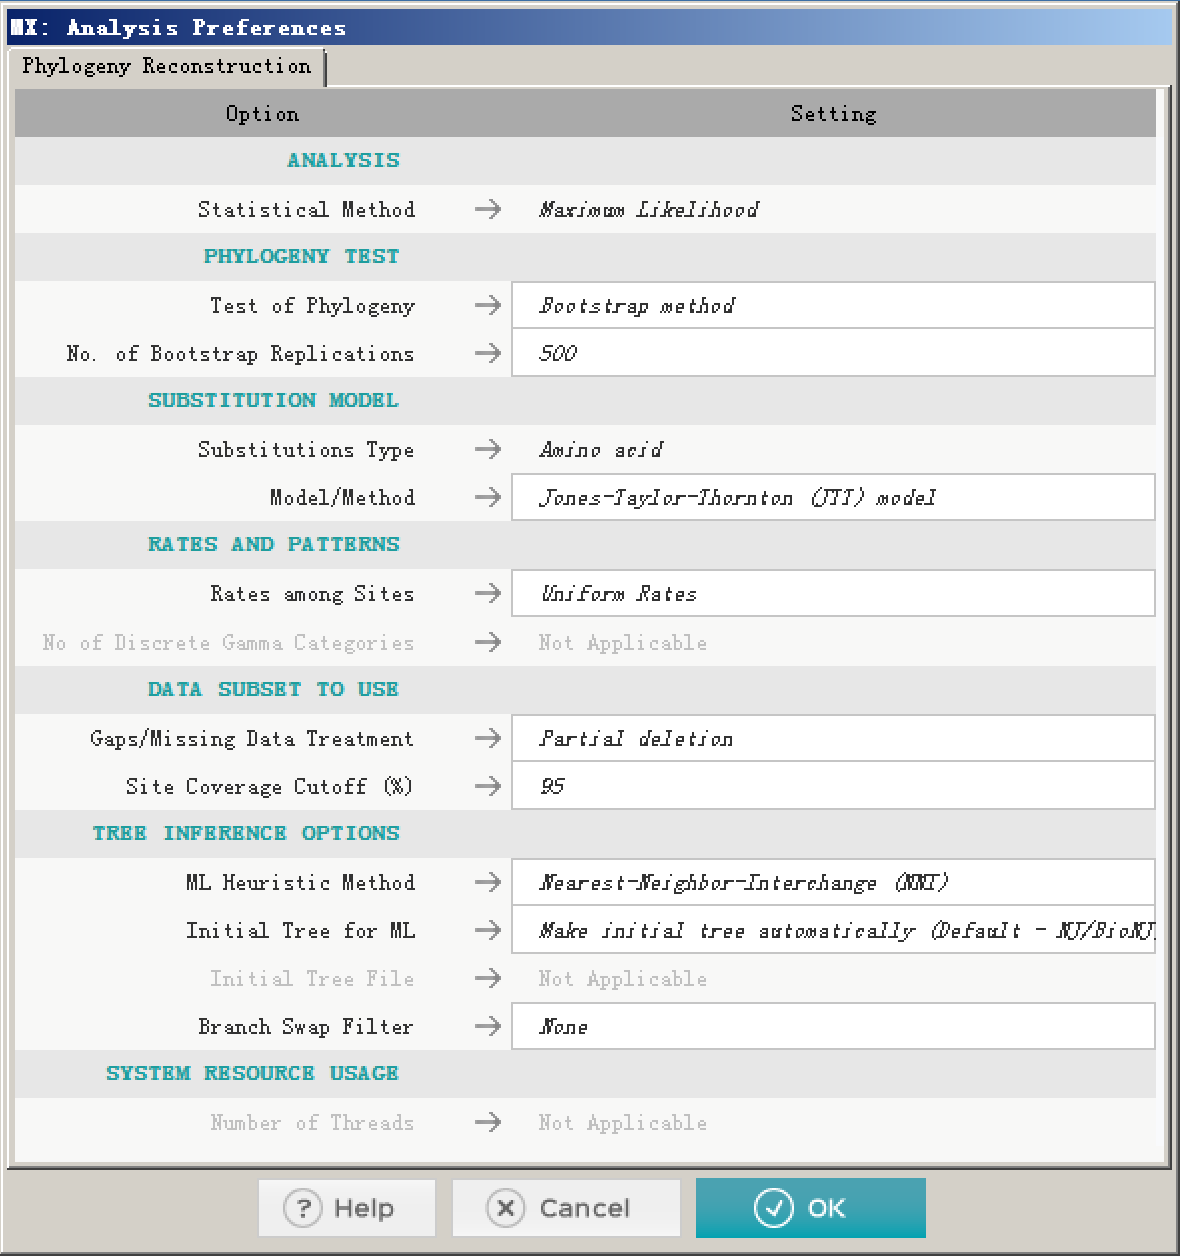
\includegraphics[width=0.5\textwidth]{image/MEGAX.png}
    \caption{Parameters of the phylogenetic tree building}
    \label{MEGAX}
\end{figure}

Then the phylogenetic tree is exported to a \texttt{.nwk} format and used in R for visualization.

\subsection{Protein physicochemical property prediction}
Protein physicochemical property prediction is done using Expasy ProtParam\upcite{gasteiger2005protein}. The complete sequence is analysed.
TMPred\upcite{hofmann1993tmbase} is also used to predict the hydrophobic region of proteins.
\subsection{Nuclear localization signal prediction}
Nuclear localization signal prediction is done using cNLS Mapper\upcite{kosugi2009systematic}, with a cut off set to 2.0.

\subsection{DNA binding site prediction for Cys2His2 zinc finger proteins}
DNA binding site prediction for Cys2His2 zinc finger proteins is done with the Interactive PWM predictor\upcite{persikov2014novo}, and the model used in this tool is expanded linear SVM\upcite{cortes1995support}.

\subsection{Transcriptome analysis}
Transcriptome analysis is done using the code derived from GEO2R. The grouping of the analysis is the same as the grouping in the GSE76510 data series.
\section{Results}

\subsection{Sequence of MTF-1 is conserved in different organisms.}

We fetched the MTF-1 gene of different eukaryotic organisms from NCBI protein database, and did a multiple sequence alignment. The organisms used in MSA and the accession number is listed in supplementary material.


The MSA showed that peptide sequence of MTF-1 is conserved in different eukaryotic organisms, as is shown in the figure below. We also built a phylogenetic tree using the MSA data as is shown in the figure below.

\begin{figure}[H]
    \centering
    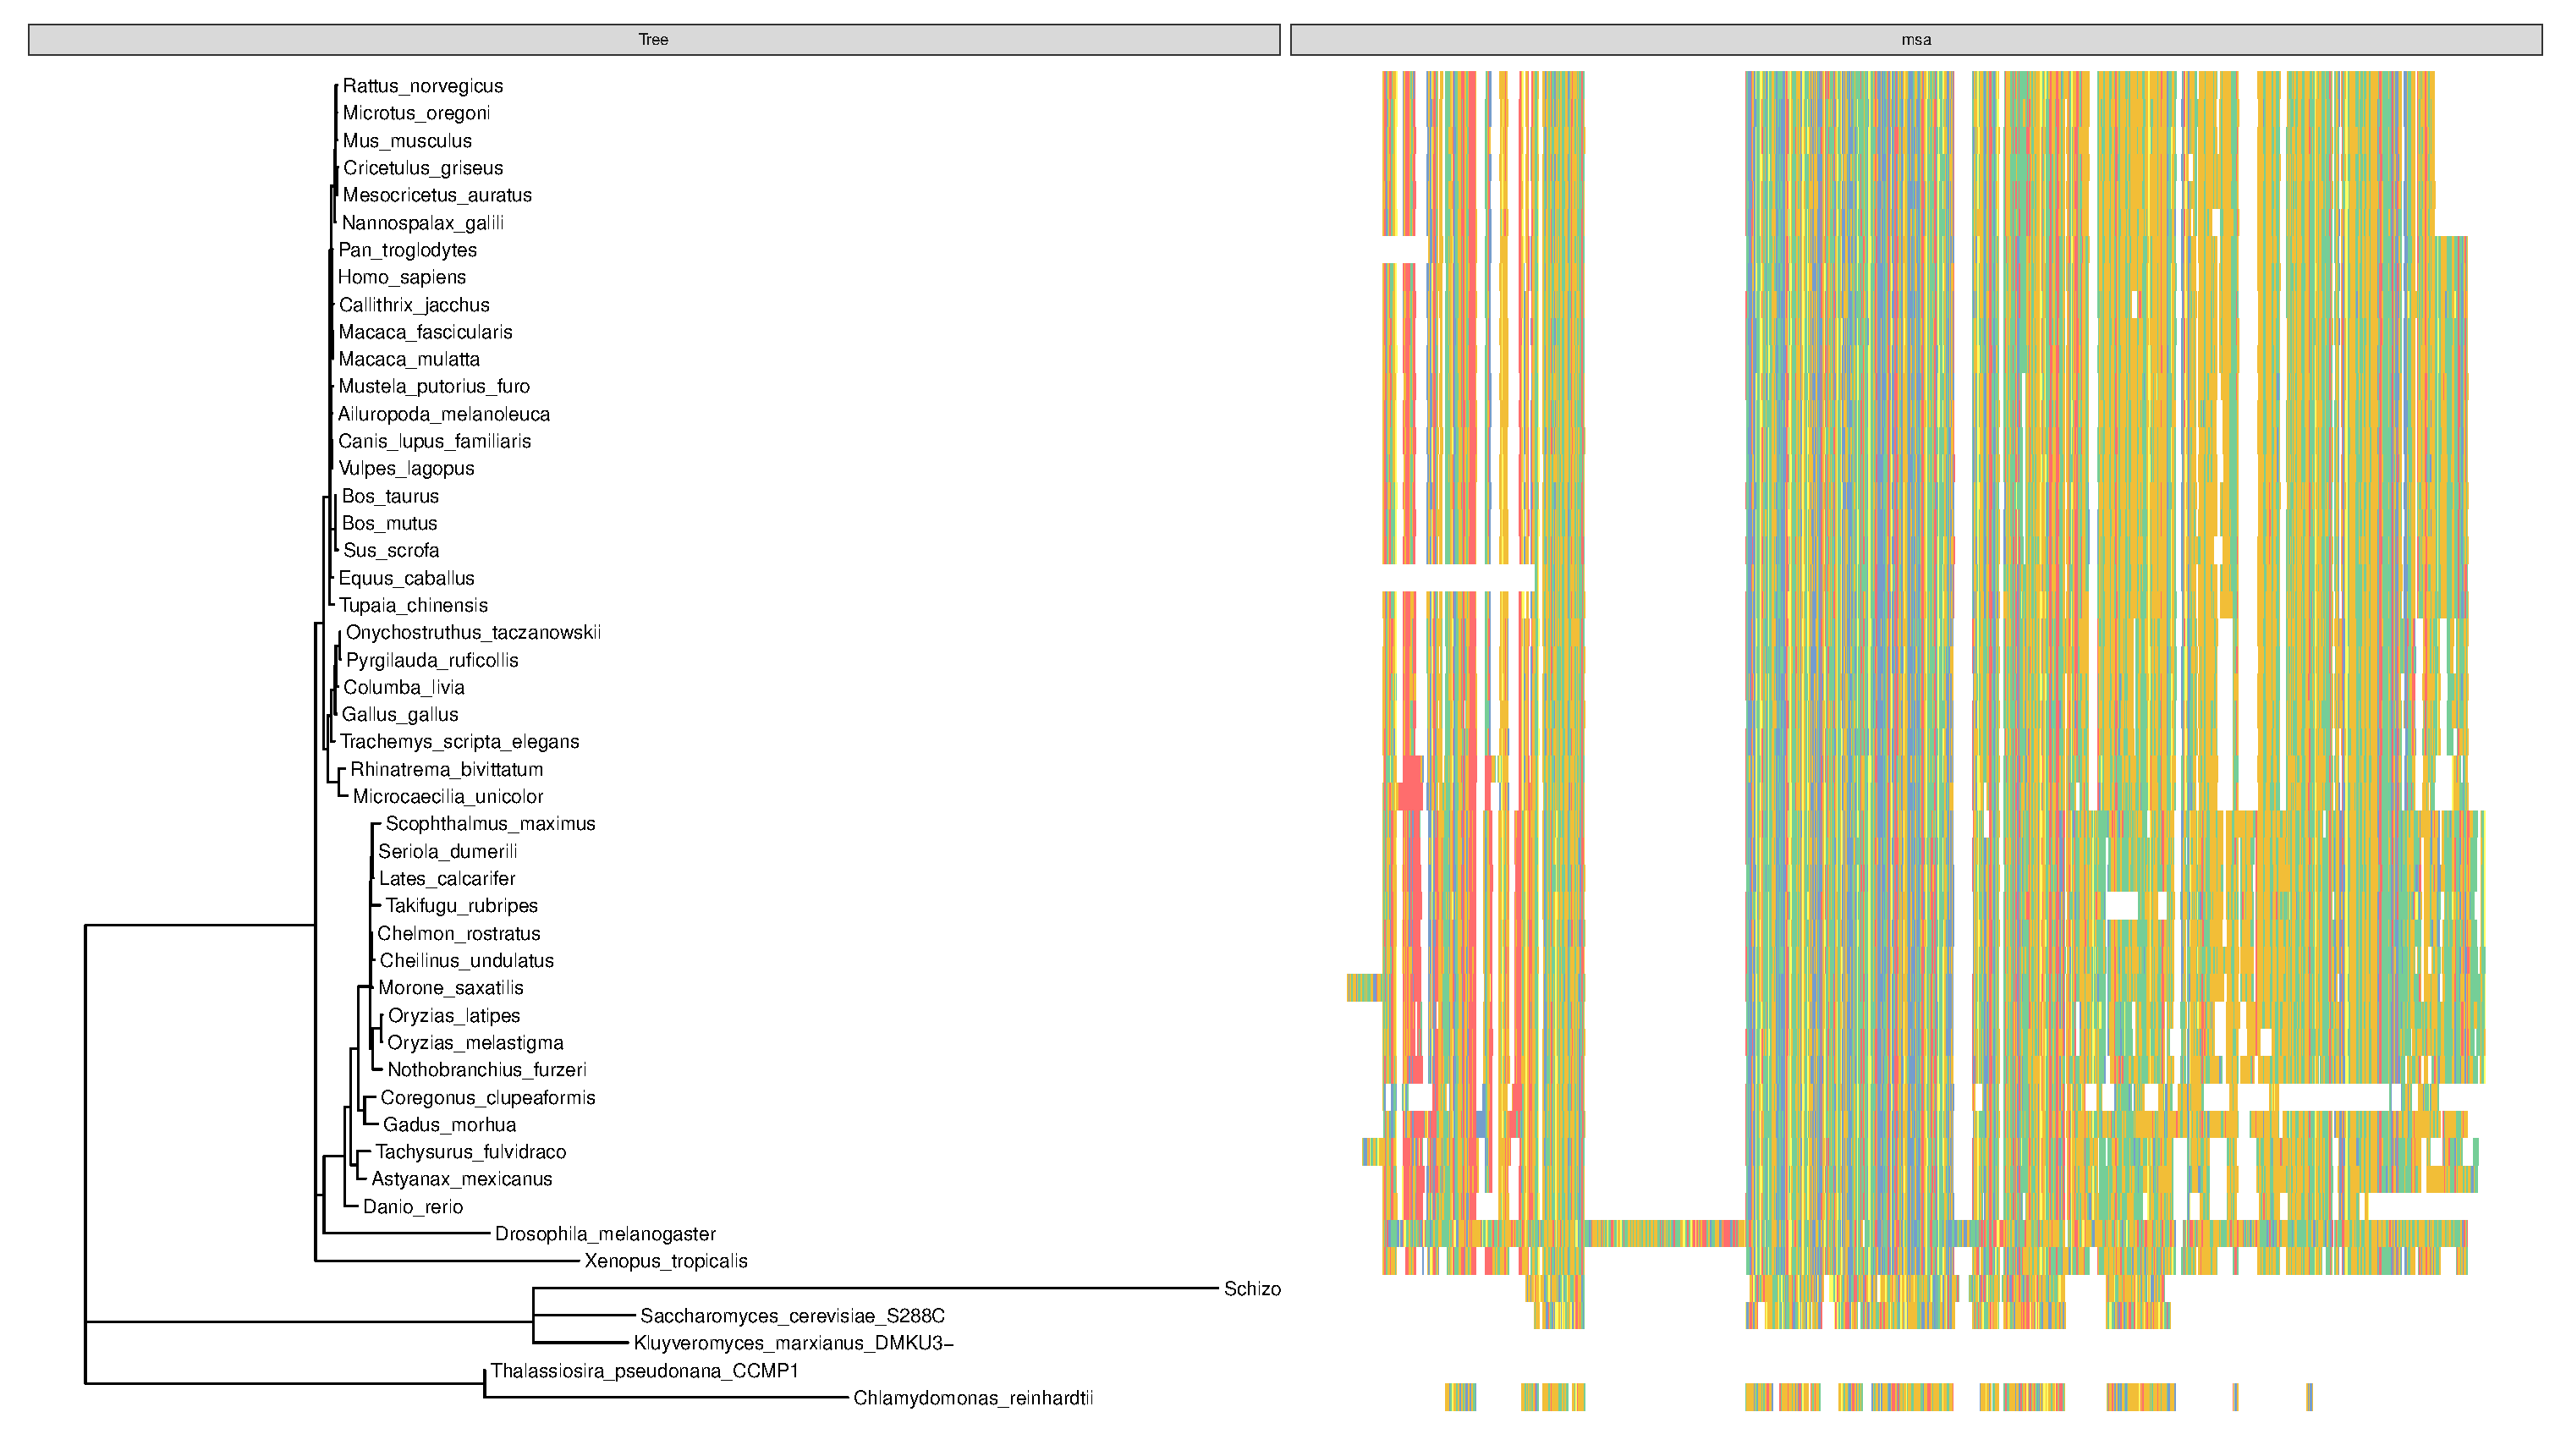
\includegraphics[width=1\textwidth]{image/MSAT.eps}
    \caption{MSA Results (right) and Phylogenetic tree (left) of MTF-1}
    \label{MSAT}
\end{figure}

From the figure, we can find that, in spite of few sequences, MTF-1 in most of the selected organism share similar peptide sequence patterns, which indicates that MTF-1 is conserved in the evolution.

As can be seen in the phylogenetic tree, \textit{Pan troglodytes} or the common chimpanzee shares the closest ancestor with humans. While the fruit fly, \textit{Drosophila melanogaster}, has distinctive MTF-1 sequence with a ~150bp insertion. These results is reasonable and consistent with previous results.

Then we analysed the nucleotide sequence of MTF-1 in the genome of different organisms, and we found that in most organisms, like \textit{Homo sapiens} and \textit{Mus musculus}, there are 7-9 exons in the MTF-1 gene, and they are spliced in a similar way. The related results of human MTF-1 is shown in the figure below.

\begin{figure}[H]
    \centering
    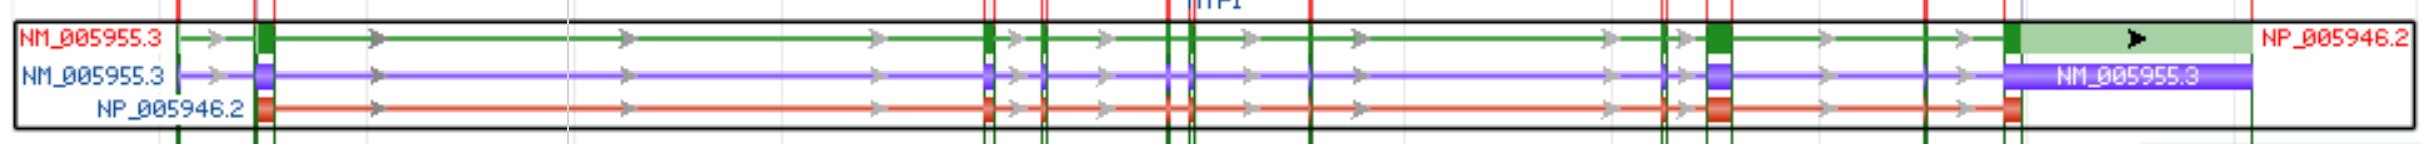
\includegraphics[width=1\textwidth]{image/MTFE.png}
    \caption{Human MTF-1 exons}
    \label{MSAT}
\end{figure}

\subsection{MTF-1 may be an unstable hydrophilic protein.}

Using Expasy ProtParam\upcite{gasteiger2005protein} to analysis mammalian MTF-1 sequences, we found that most of the MTF-1 are hydrophilic, with the average GRAVY\upcite{kyte1982simple} around -0.5. Moreover, Estimated half-life of MTF-1 in many organisms are about 30 hours, which indicates that the protein is unstable.

\begin{figure}[H]
    \centering
    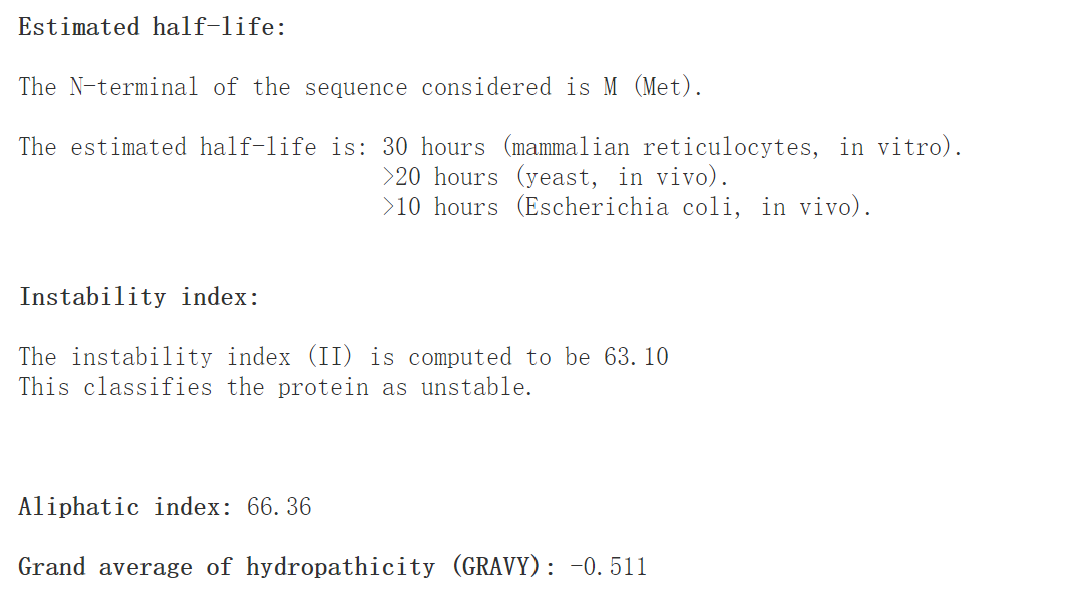
\includegraphics[width=0.7\textwidth]{image/EXPP.png}
    \caption{Part of Human MTF-1 Expasy ProtParam results}
    \label{EXPP}
\end{figure}

Detailed protparam report of human MTF-1 is shown in Supplementary material.

We also performed a TMPred analysis on human MTF-1 to find the hydrophobic region, and the output figure is shown below.

\begin{figure}[H]
    \centering
    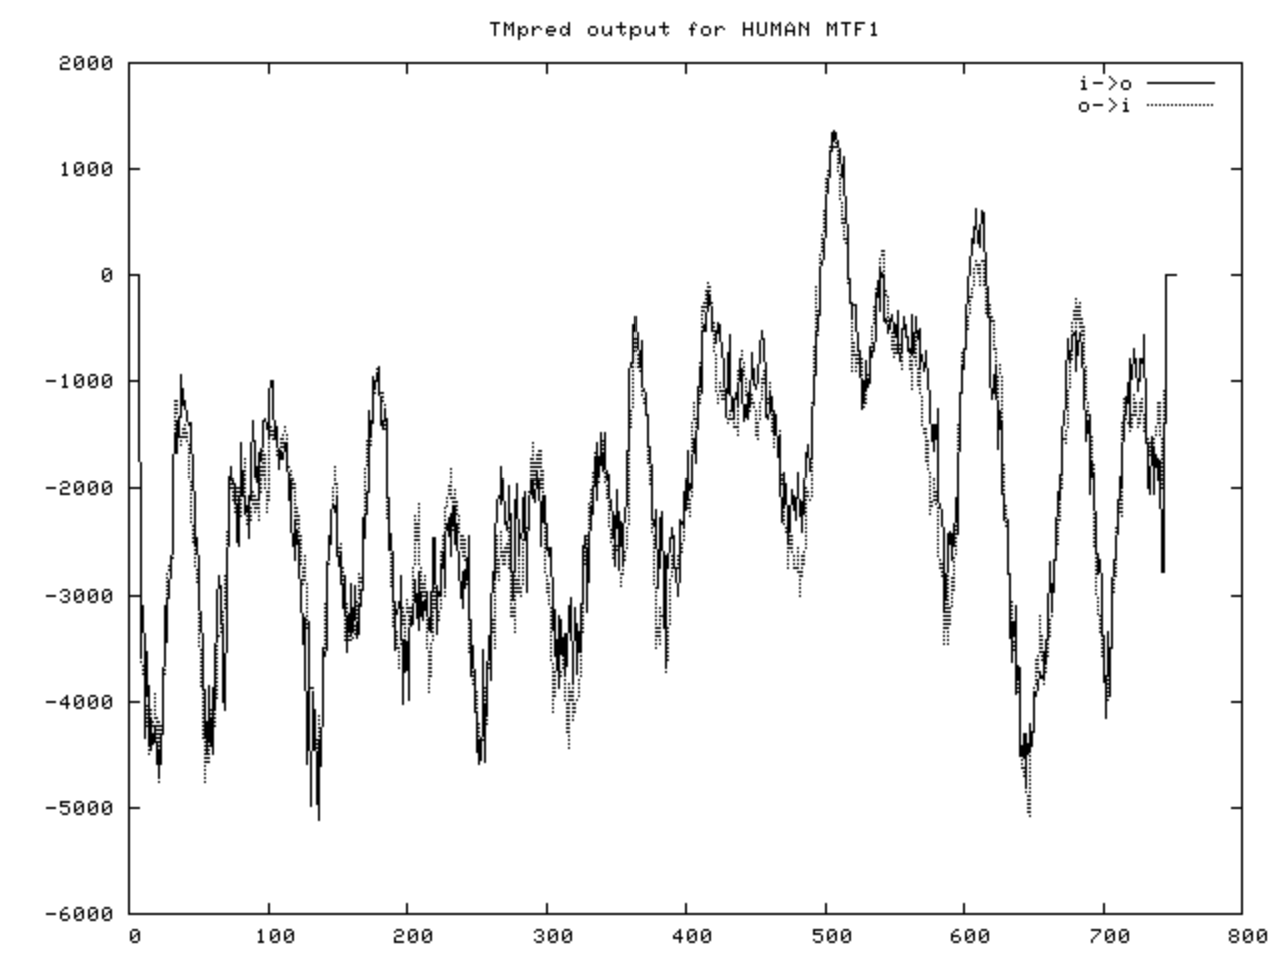
\includegraphics[width=0.7\textwidth]{image/TMPRED.png}
    \caption{Part of Human MTF-1 Expasy TMPred results}
    \label{TMPRED}
\end{figure}

Since MTF-1 is not a membrane protein, it is reasonable that no significant hydrophobic region is found.

\subsection{MTF-1 has nuclear localization signal and zinc finger domains which help it to bind metal response elements.}

Since sequence of MTF-1 is conserved in different eukaryotic organisms, we wanted to find out if there is certain motifs or domains in the MTF-1 conserved region. The sequence used in this subsection is human MTF-1.

Nuclear localization signal is found using cNLS Mapper\upcite{kosugi2009systematic}, with a cut off set to 2.0. The NLS is PETKRKEVKR, which is consistent to the manually annotated KRKEVK signal. The results given by cNLS Mapper is shown below.

\begin{figure}[H]
    \centering
    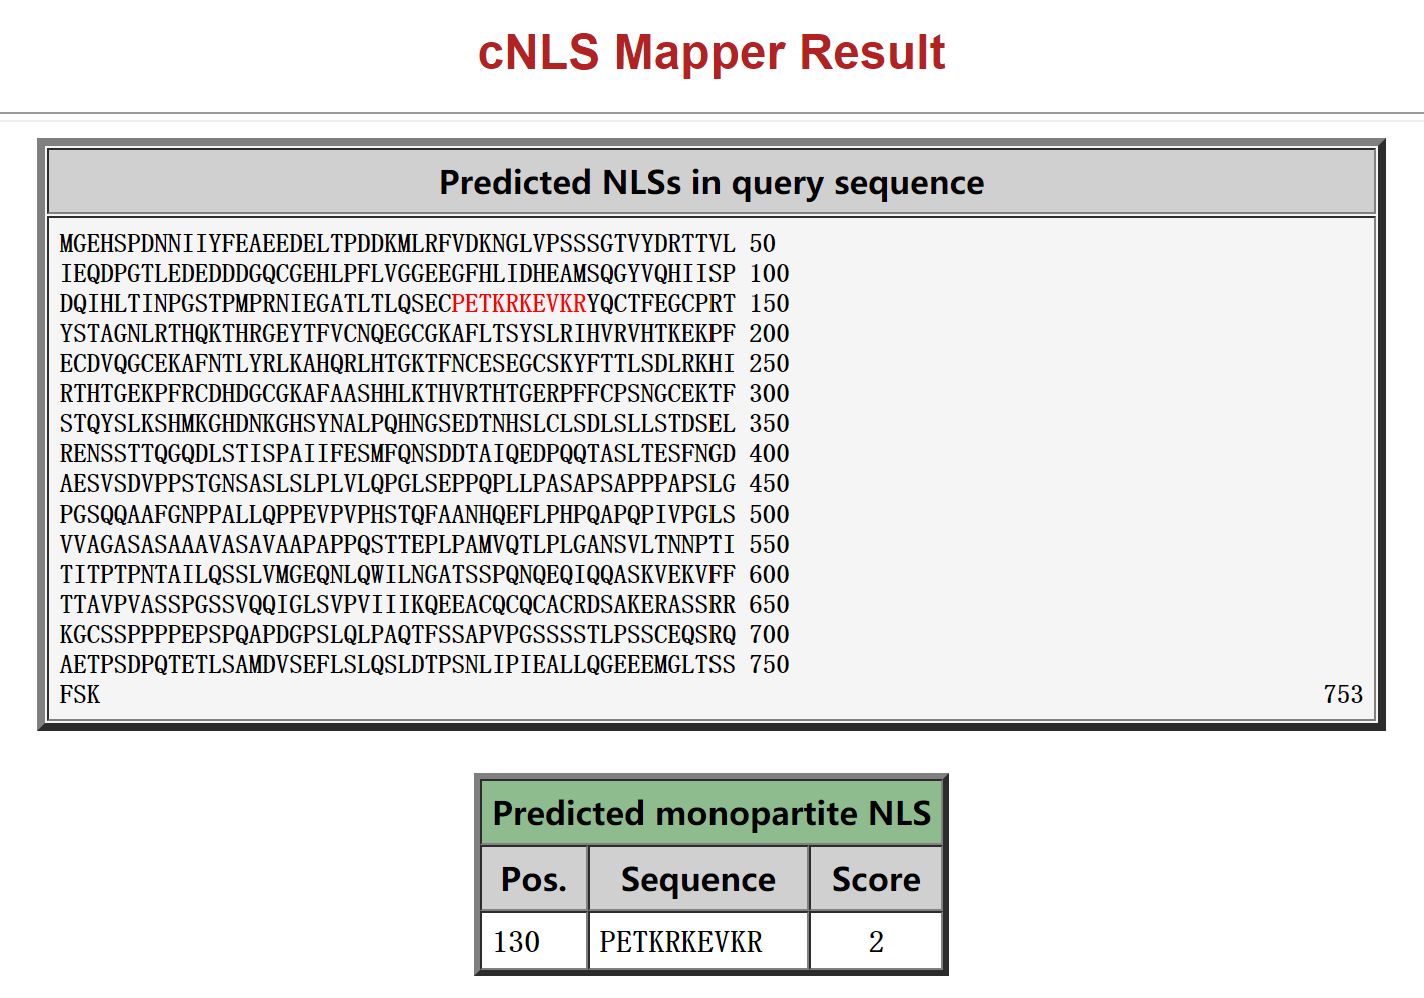
\includegraphics[width=0.7\textwidth]{image/NLSP.png}
    \caption{cNLS Mapper Results (Human MTF-1)}
    \label{NLSP}
\end{figure}

A common domain in transcription factors is the zinc finger domain, and we found 6 ZF domains in human MTF-1 protein using Interactive PWM predictor\upcite{persikov2014novo}, as is shown in the figure below.

\begin{figure}[H]
    \centering
    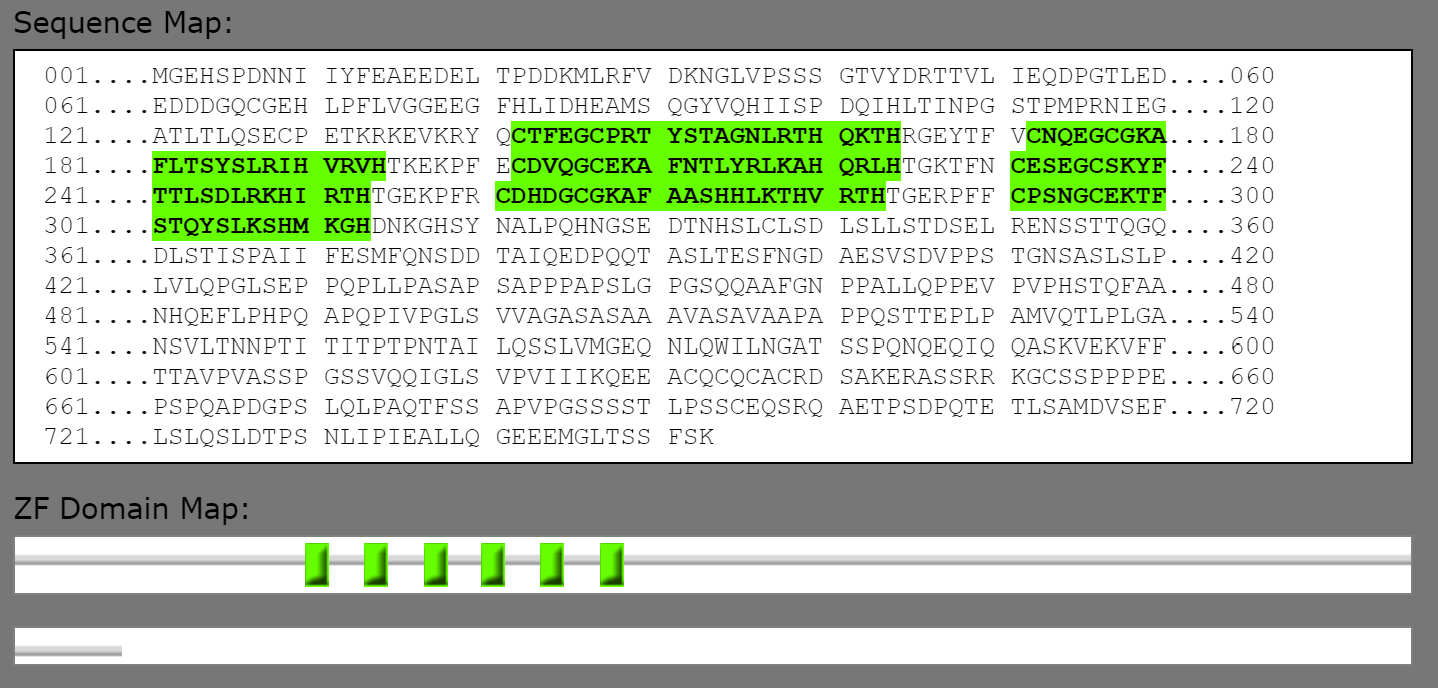
\includegraphics[width=0.7\textwidth]{image/ZFO.png}
    \caption{cNLS Mapper Results (Human MTF-1)}
    \label{HZFP}
\end{figure}

For those MTF-1 in other organisms, the similar zinc finger domain pattern can be found. Here we show \textit{Mus musculus} and \textit{Drosophila melanogaster} as examples.
\begin{figure}[H]
    \centering
    \subfigure[Mouse MTF-1] {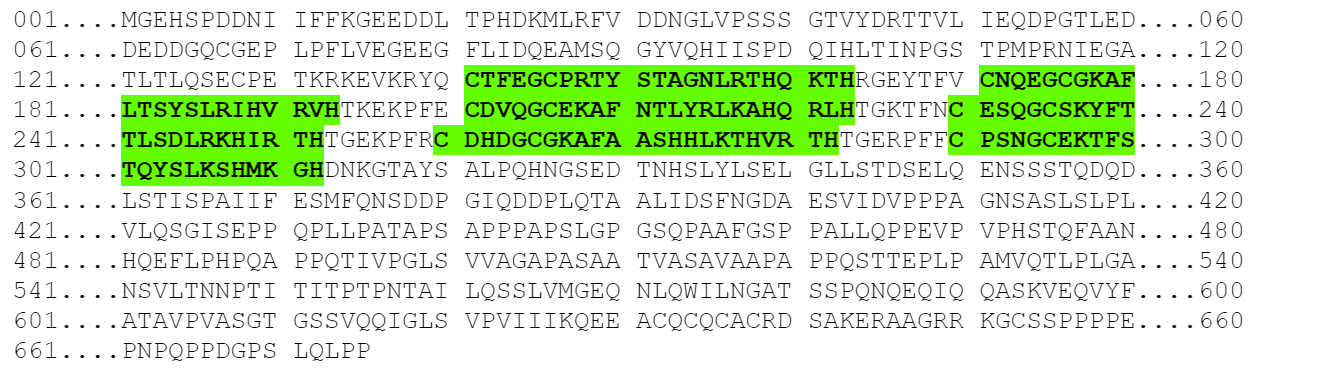
\includegraphics[width=.45\textwidth]{image/MusZF.png}}
	\subfigure[Fly MTF-1] {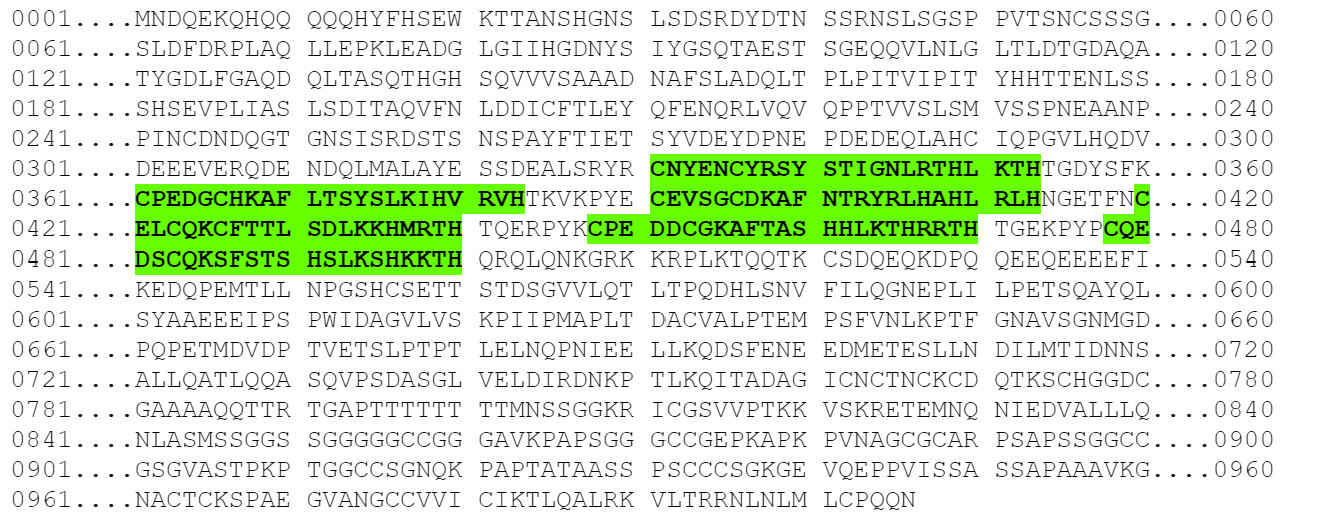
\includegraphics[width=.45\textwidth]{image/FlyZF.png}}
    \caption{Zinc finger prediction}
    \label{ZFP}
\end{figure}

Among the organisms we selected, most of them have the MTF-1 with 6 zinc finger domains, which is consistent with annotations in databases like uniprot.

\subsection{A consensus sequence named metal response elements can be found in a certain set of genes.}

Previous researches show that zinc finger can bind to a specific DNA sequence so that the protein can function on specific gene sequences. For transcription factors, zinc fingers can help them bind to the enhancers or upstream activation sequences so that they can recruit other transcription factors and RNA polymerase. Since the MTF-1 has zinc fingers, we wanted to know what sequence it can bind.

We used Interactive PWM Predictor, the DNA binding site predictor for Cys2His2 Zinc Finger Proteins\upcite{persikov2014novo}, to predict the binding sequence of MTF-1, and the results is shown below.

\begin{figure}[H]
    \centering
    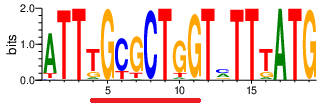
\includegraphics[width=0.9\textwidth]{image/seq_logo.png}
    \caption{Zinc finger binding sequence prediction}
    \label{ZCP}
\end{figure}

The detailed PWM can be found in Supplementary Material. From the figure above, we can find that the predicted consensus sequence is close to TGCRCNC reported in previous literature, indicating that this sequence is related to the function of MTF-1.

In other organisms, like \textit{Mus musculus} and \textit{Drosophila melanogaster}, the consensus sequence is highly similar.

\subsection{Expression of a certain set of genes with metal response elements may be regulated by MTF-1.}

We searched the human genome for the consensus sequence TGCRCNC, and 588381 hits are found. Among these hits, 126415 are close to an exon. We then compared the data to the annotation and gene ontology, and found several genes that can possibly be regulated by MTF-1 via the consensus sequence named metal response elements. These genes are listed below.

\begin{enumerate}
    \item MT/metallothionein
    \item HAMP/hepcidin
    \item PRNP/major prion protein
    \item DDAH1/N(G),N(G)-dimethylarginine dimethylaminohydrolase 1
\end{enumerate}

Then we did an analysis on the data series GSE76510\upcite{hardyman2016zinc} from GEO, which is a data set collected using Illumina HumanHT-12 V4.0 expression beadchip. In the experiment, a targeted siRNA was used to deplete MTF1 expression in the human intestinal cell line Caco-2, so that when the cell are treated with different zinc level, we can observe the difference in gene expression between the MTF-1 knockdown group and the control group. In this way, we can get more understanding of the MTF-1 regulated zinc-responsive genes expression.

The top differently expressed genes are listed below.

\begin{enumerate}
    \item HSPA6: heat shock protein family A (Hsp70) member 6
    \item MT1E:	metallothionein 1E
    \item MT1H:	metallothionein 1H
    \item RNA5S9:	RNA, 5S ribosomal 9
    \item MT1M:	metallothionein 1M
    \item SNORD3A:	small nucleolar RNA, C/D box 3A
    \item SNORD3D:	small nucleolar RNA, C/D box 3D
    \item MT1B:	metallothionein 1B
    \item MT1A:	metallothionein 1A
    \item SNORD3C:	small nucleolar RNA, C/D box 3C
    \item RN7SK:	RNA, 7SK small nuclear
    \item MT1F:	metallothionein 1F
    \item MT1G:	metallothionein 1G
    \item SERPINE2:	serpin family E member 2
    \item MT2A:	metallothionein 2A
    \item SLC30A1:	solute carrier family 30 member 1
    \item MT1X:	metallothionein 1X
    \item HSPA1A:	heat shock protein family A (Hsp70) member 1A
\end{enumerate}

Metallothioneins, as well as other genes, seem to be related to the change in MTF-1, which suggests that expression of a certain set of genes may be regulated by MTF-1. Some of them have metal response elements upstream several kbs of the gene.
\section{Discussion \& Conclusions}

We started our analysis from the multiple sequence alignment of MTF-1 protein sequence in different organisms and find out that protein sequence of MTF-1 is conserved in different organisms. We then analysed the nucleotide sequence of MTF-1, and found that the exon and intron patterns share a high similarity among these organisms.

Similar sequence indicates that similar feathers and functions exist. Therefore we did analysis on the physicochemical properties of MTF-1 in in different organisms, and the results are consistent with our initial guess.

To study the function of MTF-1, we first checked the sequence for special domains. Nuclear localization signal and Zinc finger domain are found, which suggests that MTF-1 works like a transcription factor. Since the zinc finger domains can recognize and bind to specific DNA sequences, we would like to know what the target sequences are. Fortunately, suitable tools are published and we are able to get the consensus sequence of MTF-1 target/binding sequences.

With the MTF-1 target/binding sequences, the question about what genes are regulated via the MTF-1 target/binding sequences (that is, metal response elements MREs) formed. Through sequence screening and transcriptome analysis, several genes that are likely to be regulated by MTF-1 is found.

Still, we do not know the exact structure of the MTF-1, since homologous modeling of MTF-1 fails to give out reasonable structures. \textit{Ab initio} methods, however, cost too much time and computation resources for facilities to afford. Considering that MTF-1 is an unstable protein, elucidation opf its structure by X-ray crystallography may face difficulties, and other methods, like NMR, is not suitable for such a large protein. Cryoelectron Microscopy might be a choice for this task, butin our literature review, no relevant work was found.

If we have the exact structure of the MTF-1, many processes involving MTF-1 will be studied more deeply, and we can gain more insight into the mechanisms of metal regulatory transcription factor, including but not limited to MTF-1.
\section{Acknowledgment}

Throughout the writing of this report I have received a great deal of support and assistance.

I would like to thank the teachers of the course, whose expertise was invaluable in formulating the research questions and methodology. 

I would also like to acknowledge my classmates in this course for their wonderful collaboration. I would particularly like to single out Zhifan Lin, I want to thank you for your patient support and insightful suggestions.

\section*{Supplementary Material}

\subsection*{Accession number of sequences and GEO data set}
The accession number of sequences are listed below.
\begin{lstlisting}[basicstyle=\tiny\ttfamily]
>NP_032662.3 Mtf1 [organism=Mus musculus] [GeneID=17764]
>NP_001097560.1 MTF-1 [organism=Drosophila melanogaster] [GeneID=39089] [isoform=C ]
>NP_001097561.1 MTF-1 [organism=Drosophila melanogaster] [GeneID=39089] [isoform=D ]
>NP_001097562.1 MTF-1 [organism=Drosophila melanogaster] [GeneID=39089] [isoform=E ]
>NP_001287002.1 MTF-1 [organism=Drosophila melanogaster] [GeneID=39089] [isoform=F ]
>NP_001287003.1 MTF-1 [organism=Drosophila melanogaster] [GeneID=39089] [isoform=G ]
>NP_648311.2 MTF-1 [organism=Drosophila melanogaster] [GeneID=39089] [isoform=A ]
>NP_729491.1 MTF-1 [organism=Drosophila melanogaster] [GeneID=39089] [isoform=B ]
>NP_001027866.1 mtf1 [organism=Takifugu rubripes] [GeneID=446075]
>XP_029694032.1 mtf1 [organism=Takifugu rubripes] [GeneID=446075] [isoform=X1]
>XP_029694033.1 mtf1 [organism=Takifugu rubripes] [GeneID=446075] [isoform=X1]
>XP_029694034.1 mtf1 [organism=Takifugu rubripes] [GeneID=446075] [isoform=X2]
>XP_029694035.1 mtf1 [organism=Takifugu rubripes] [GeneID=446075] [isoform=X3]
>XP_029694036.1 mtf1 [organism=Takifugu rubripes] [GeneID=446075] [isoform=X4]
>XP_029694037.1 mtf1 [organism=Takifugu rubripes] [GeneID=446075] [isoform=X5]
>XP_029694038.1 mtf1 [organism=Takifugu rubripes] [GeneID=446075] [isoform=X6]
>XP_029694039.1 mtf1 [organism=Takifugu rubripes] [GeneID=446075] [isoform=X7]
>NP_005946.2 MTF1 [organism=Homo sapiens] [GeneID=4520]
>XP_011539793.1 MTF1 [organism=Homo sapiens] [GeneID=4520] [isoform=X1]
>XP_011539795.1 MTF1 [organism=Homo sapiens] [GeneID=4520] [isoform=X2]
>XP_011539796.1 MTF1 [organism=Homo sapiens] [GeneID=4520] [isoform=X3]
>NP_013955.1 MTF1 [organism=Saccharomyces cerevisiae S288C] [GeneID=855268]
>XP_027004713.1 mtf1 [organism=Tachysurus fulvidraco] [GeneID=113644242] [isoform=X1]
>XP_027004715.1 mtf1 [organism=Tachysurus fulvidraco] [GeneID=113644242] [isoform=X2]
>XP_027004716.1 mtf1 [organism=Tachysurus fulvidraco] [GeneID=113644242] [isoform=X3]
>XP_027004717.1 mtf1 [organism=Tachysurus fulvidraco] [GeneID=113644242] [isoform=X3]
>XP_027004718.1 mtf1 [organism=Tachysurus fulvidraco] [GeneID=113644242] [isoform=X3]
>NP_694513.1 mtf1 [organism=Danio rerio] [GeneID=195821]
>XP_021322285.1 mtf1 [organism=Danio rerio] [GeneID=195821] [isoform=X1]
>XP_021322286.1 mtf1 [organism=Danio rerio] [GeneID=195821] [isoform=X2]
>NP_593495.1 mtf1 [organism=Schizosaccharomyces pombe] [GeneID=2543271]
>NP_001102147.1 Mtf1 [organism=Rattus norvegicus] [GeneID=362591]
>XP_006238946.1 Mtf1 [organism=Rattus norvegicus] [GeneID=362591] [isoform=X1]
>XP_038966270.1 Mtf1 [organism=Rattus norvegicus] [GeneID=362591] [isoform=X2]
>XP_038966271.1 Mtf1 [organism=Rattus norvegicus] [GeneID=362591] [isoform=X3]
>XP_038966272.1 Mtf1 [organism=Rattus norvegicus] [GeneID=362591] [isoform=X4]
>NP_001026666.1 MTF1 [organism=Gallus gallus] [GeneID=428218]
>XP_015153181.1 MTF1 [organism=Gallus gallus] [GeneID=428218] [isoform=X2]
>XP_040507666.1 MTF1 [organism=Gallus gallus] [GeneID=428218] [isoform=X1]
>XP_040507667.1 MTF1 [organism=Gallus gallus] [GeneID=428218] [isoform=X1]
>NP_001267060.1 MTF1 [organism=Pan troglodytes] [GeneID=456766]
>XP_009451322.1 MTF1 [organism=Pan troglodytes] [GeneID=456766] [isoform=X1]
>XP_016806813.1 MTF1 [organism=Pan troglodytes] [GeneID=456766] [isoform=X1]
>XP_016806894.1 MTF1 [organism=Pan troglodytes] [GeneID=456766] [isoform=X3]
>XP_024202793.1 MTF1 [organism=Pan troglodytes] [GeneID=456766] [isoform=X2]
>NP_001030252.2 MTF1 [organism=Bos taurus] [GeneID=509960]
>XP_005204750.1 MTF1 [organism=Bos taurus] [GeneID=509960] [isoform=X1]
>NP_001244724.1 MTF1 [organism=Macaca mulatta] [GeneID=714795]
>XP_014991031.1 MTF1 [organism=Macaca mulatta] [GeneID=714795] [isoform=X1]
>XP_014991038.1 MTF1 [organism=Macaca mulatta] [GeneID=714795] [isoform=X1]
>XP_028701043.1 MTF1 [organism=Macaca mulatta] [GeneID=714795] [isoform=X2]
>XP_002291569.1 MTF1 [organism=Thalassiosira pseudonana CCMP1335] [GeneID=7442748]
>XP_002939525.1 mtf1 [organism=Xenopus tropicalis] [GeneID=100495484]
>XP_012812846.1 mtf1 [organism=Xenopus tropicalis] [GeneID=100495484]
>XP_031752770.1 mtf1 [organism=Xenopus tropicalis] [GeneID=100495484]
>XP_004740804.1 MTF1 [organism=Mustela putorius furo] [GeneID=101690205] [isoform=X1]
>XP_004740805.1 MTF1 [organism=Mustela putorius furo] [GeneID=101690205] [isoform=X2]
>XP_005543973.1 MTF1 [organism=Macaca fascicularis] [GeneID=101926816]
>XP_005543974.1 MTF1 [organism=Macaca fascicularis] [GeneID=101926816]
>XP_005543975.1 MTF1 [organism=Macaca fascicularis] [GeneID=101926816]
>XP_001703129.1 MTF1 [organism=Chlamydomonas reinhardtii] [GeneID=5728690]
>XP_005628986.1 MTF1 [organism=Canis lupus familiaris] [GeneID=608127] [isoform=X3]
>XP_005628987.1 MTF1 [organism=Canis lupus familiaris] [GeneID=608127] [isoform=X3]
>XP_013975033.1 MTF1 [organism=Canis lupus familiaris] [GeneID=608127] [isoform=X2]
>XP_022283522.1 MTF1 [organism=Canis lupus familiaris] [GeneID=608127] [isoform=X1]
>XP_038351419.1 MTF1 [organism=Canis lupus familiaris] [GeneID=608127] [isoform=X1]
>XP_038351420.1 MTF1 [organism=Canis lupus familiaris] [GeneID=608127] [isoform=X2]
>XP_038351421.1 MTF1 [organism=Canis lupus familiaris] [GeneID=608127] [isoform=X3]
>XP_038351422.1 MTF1 [organism=Canis lupus familiaris] [GeneID=608127] [isoform=X3]
>XP_038413769.1 MTF1 [organism=Canis lupus familiaris] [GeneID=608127] [isoform=X1]
>XP_038413770.1 MTF1 [organism=Canis lupus familiaris] [GeneID=608127] [isoform=X2]
>XP_038413771.1 MTF1 [organism=Canis lupus familiaris] [GeneID=608127] [isoform=X3]
>XP_038413772.1 MTF1 [organism=Canis lupus familiaris] [GeneID=608127] [isoform=X3]
>XP_038477644.1 MTF1 [organism=Canis lupus familiaris] [GeneID=608127] [isoform=X1]
>XP_038477645.1 MTF1 [organism=Canis lupus familiaris] [GeneID=608127] [isoform=X2]
>XP_038477646.1 MTF1 [organism=Canis lupus familiaris] [GeneID=608127] [isoform=X3]
>XP_038477647.1 MTF1 [organism=Canis lupus familiaris] [GeneID=608127] [isoform=X3]
>XP_038543415.1 MTF1 [organism=Canis lupus familiaris] [GeneID=608127] [isoform=X1]
>XP_038543416.1 MTF1 [organism=Canis lupus familiaris] [GeneID=608127] [isoform=X2]
>XP_038543417.1 MTF1 [organism=Canis lupus familiaris] [GeneID=608127] [isoform=X3]
>XP_038543418.1 MTF1 [organism=Canis lupus familiaris] [GeneID=608127] [isoform=X3]
>XP_011228926.1 MTF1 [organism=Ailuropoda melanoleuca] [GeneID=100480003] [isoform=X2]
>XP_034505425.1 MTF1 [organism=Ailuropoda melanoleuca] [GeneID=100480003] [isoform=X1]
>XP_034505435.1 MTF1 [organism=Ailuropoda melanoleuca] [GeneID=100480003] [isoform=X3]
>XP_034505440.1 MTF1 [organism=Ailuropoda melanoleuca] [GeneID=100480003] [isoform=X4]
>NP_001230473.1 MTF1 [organism=Sus scrofa] [GeneID=100511998]
>XP_020948959.1 MTF1 [organism=Sus scrofa] [GeneID=100511998] [isoform=X1]
>XP_020948960.1 MTF1 [organism=Sus scrofa] [GeneID=100511998] [isoform=X2]
>XP_005084415.1 Mtf1 [organism=Mesocricetus auratus] [GeneID=101832232] [isoform=X1]
>XP_012979330.1 Mtf1 [organism=Mesocricetus auratus] [GeneID=101832232] [isoform=X2]
>XP_005509709.1 MTF1 [organism=Columba livia] [GeneID=102092487]
>XP_006158647.1 MTF1 [organism=Tupaia chinensis] [GeneID=102475717] [isoform=X1]
>XP_006158648.1 MTF1 [organism=Tupaia chinensis] [GeneID=102475717] [isoform=X2]
>XP_014447108.1 MTF1 [organism=Tupaia chinensis] [GeneID=102475717] [isoform=X3]
>XP_027255030.1 Mtf1 [organism=Cricetulus griseus] [GeneID=100752132] [isoform=X3]
>XP_035295521.1 Mtf1 [organism=Cricetulus griseus] [GeneID=100752132]
>XP_035295522.1 Mtf1 [organism=Cricetulus griseus] [GeneID=100752132]
>XP_035311622.1 Mtf1 [organism=Cricetulus griseus] [GeneID=100752132] [isoform=X1]
>XP_005893304.1 MTF1 [organism=Bos mutus] [GeneID=102267771]
>XP_008848440.2 Mtf1 [organism=Nannospalax galili] [GeneID=103747698]
>XP_035479853.1 mtf1 [organism=Scophthalmus maximus] [GeneID=118299875] [isoform=X1]
>XP_035479862.1 mtf1 [organism=Scophthalmus maximus] [GeneID=118299875] [isoform=X1]
>XP_035479869.1 mtf1 [organism=Scophthalmus maximus] [GeneID=118299875] [isoform=X2]
>XP_022676757.1 MTF1 [organism=Kluyveromyces marxianus DMKU3-1042] [GeneID=34716899]
>XP_018554070.1 mtf1 [organism=Lates calcarifer] [GeneID=108898617] [isoform=X1]
>XP_018554076.1 mtf1 [organism=Lates calcarifer] [GeneID=108898617] [isoform=X2]
>XP_022619994.1 mtf1 [organism=Seriola dumerili] [GeneID=111235748]
>XP_024122982.1 mtf1 [organism=Oryzias melastigma] [GeneID=112143331]
>XP_036071630.1 mtf1 [organism=Oryzias melastigma] [GeneID=112143331]
>XP_034609894.1 MTF1 [organism=Trachemys scripta elegans] [GeneID=117868217] [isoform=X1]
>XP_034609896.1 MTF1 [organism=Trachemys scripta elegans] [GeneID=117868217] [isoform=X2]
>XP_035527910.1 mtf1 [organism=Morone saxatilis] [GeneID=118335622]
>XP_014592828.1 MTF1 [organism=Equus caballus] [GeneID=100054605] [isoform=X3]
>XP_023488944.1 MTF1 [organism=Equus caballus] [GeneID=100054605] [isoform=X1]
>XP_023488948.1 MTF1 [organism=Equus caballus] [GeneID=100054605] [isoform=X2]
>XP_035106762.1 MTF1 [organism=Callithrix jacchus] [GeneID=100397778]
>XP_035106763.1 MTF1 [organism=Callithrix jacchus] [GeneID=100397778]
>XP_035106764.1 MTF1 [organism=Callithrix jacchus] [GeneID=100397778]
>XP_035106765.1 MTF1 [organism=Callithrix jacchus] [GeneID=100397778]
>XP_035106766.1 MTF1 [organism=Callithrix jacchus] [GeneID=100397778]
>XP_015805577.1 mtf1 [organism=Nothobranchius furzeri] [GeneID=107379368]
>XP_015805578.1 mtf1 [organism=Nothobranchius furzeri] [GeneID=107379368]
>XP_029476006.1 MTF1 [organism=Rhinatrema bivittatum] [GeneID=115100996] [isoform=X1]
>XP_029476007.1 MTF1 [organism=Rhinatrema bivittatum] [GeneID=115100996] [isoform=X2]
>XP_030073227.1 MTF1 [organism=Microcaecilia unicolor] [GeneID=115479457] [isoform=X1]
>XP_030073228.1 MTF1 [organism=Microcaecilia unicolor] [GeneID=115479457] [isoform=X2]
>XP_023819652.1 mtf1 [organism=Oryzias latipes] [GeneID=101170051]
>XP_023819653.1 mtf1 [organism=Oryzias latipes] [GeneID=101170051]
>XP_007249672.2 mtf1 [organism=Astyanax mexicanus] [GeneID=103028867] [isoform=X2]
>XP_022529461.1 mtf1 [organism=Astyanax mexicanus] [GeneID=103028867] [isoform=X1]
>XP_022529462.1 mtf1 [organism=Astyanax mexicanus] [GeneID=103028867] [isoform=X2]
>XP_030225509.1 mtf1 [organism=Gadus morhua] [GeneID=115553426] [isoform=X1]
>XP_030225510.1 mtf1 [organism=Gadus morhua] [GeneID=115553426] [isoform=X1]
>XP_030225511.1 mtf1 [organism=Gadus morhua] [GeneID=115553426] [isoform=X2]
>XP_041759586.1 mtf1 [organism=Coregonus clupeaformis] [GeneID=121586717]
>XP_041799057.1 mtf1 [organism=Chelmon rostratus] [GeneID=121610828] [isoform=X1]
>XP_041799058.1 mtf1 [organism=Chelmon rostratus] [GeneID=121610828] [isoform=X2]
>XP_041273270.1 MTF1 [organism=Onychostruthus taczanowskii] [GeneID=121342731] [isoform=X1]
>XP_041273271.1 MTF1 [organism=Onychostruthus taczanowskii] [GeneID=121342731] [isoform=X2]
>XP_041335250.1 MTF1 [organism=Pyrgilauda ruficollis] [GeneID=121359929] [isoform=X1]
>XP_041335251.1 MTF1 [organism=Pyrgilauda ruficollis] [GeneID=121359929] [isoform=X1]
>XP_041335252.1 MTF1 [organism=Pyrgilauda ruficollis] [GeneID=121359929] [isoform=X2]
>XP_041508025.1 Mtf1 [organism=Microtus oregoni] [GeneID=121448240] [isoform=X1]
>XP_041508027.1 Mtf1 [organism=Microtus oregoni] [GeneID=121448240] [isoform=X2]
>XP_041594242.1 MTF1 [organism=Vulpes lagopus] [GeneID=121481180] [isoform=X1]
>XP_041594243.1 MTF1 [organism=Vulpes lagopus] [GeneID=121481180] [isoform=X2]
>XP_041648790.1 mtf1 [organism=Cheilinus undulatus] [GeneID=121513247]
>XP_041648791.1 mtf1 [organism=Cheilinus undulatus] [GeneID=121513247]

>NC_000070.7:124696342-124743593 Mtf1 [organism=Mus musculus] [GeneID=17764] [chromosome=4]
>NT_037436.4:9430312-9439490 MTF-1 [organism=Drosophila melanogaster] [GeneID=39089] [chromosome=3L]
>NC_042291.1:139200-149251 mtf1 [organism=Takifugu rubripes] [GeneID=446075] [chromosome=7]
>NC_000001.11:c37859614-37809570 MTF1 [organism=Homo sapiens] [GeneID=4520] [chromosome=1]
>NC_001145.3:724626-725651 MTF1 [organism=Saccharomyces cerevisiae S288C] [GeneID=855268] [chromosome=XIII]
>NW_020847794.1:10224324-10237432 mtf1 [organism=Tachysurus fulvidraco] [GeneID=113644242] [chromosome=Un]
>NC_007127.7:4133793-4168891 mtf1 [organism=Danio rerio] [GeneID=195821] [chromosome=16]
>NC_003424.3:c1811361-1809480 mtf1 [organism=Schizosaccharomyces pombe] [GeneID=2543271] [chromosome=I]
>NC_051340.1:137062319-137107136 Mtf1 [organism=Rattus norvegicus] [GeneID=362591] [chromosome=5]
>NC_052554.1:3910145-3928852 MTF1 [organism=Gallus gallus] [GeneID=428218] [chromosome=23]
>NC_052595.1:3676675-3689106 MTF1 [organism=Gallus gallus] [GeneID=428218] [chromosome=23]
>NC_036879.1:c36645508-36594285 MTF1 [organism=Pan troglodytes] [GeneID=456766] [chromosome=1]
>NC_037330.1:108062883-108103486 MTF1 [organism=Bos taurus] [GeneID=509960] [chromosome=3]
>NC_041754.1:186717897-186771162 MTF1 [organism=Macaca mulatta] [GeneID=714795] [chromosome=1]
>NC_012069.1:c1506659-1505646 MTF1 [organism=Thalassiosira pseudonana CCMP1335] [GeneID=7442748] [chromosome=6]
>NC_030678.2:c83702964-83681607 mtf1 [organism=Xenopus tropicalis] [GeneID=100495484] [chromosome=2]
>NW_004569147.1:10639932-10681663 MTF1 [organism=Mustela putorius furo] [GeneID=101690205] [chromosome=Un]
>NC_022272.1:189948728-190000694 MTF1 [organism=Macaca fascicularis] [GeneID=101926816] [chromosome=1]
>NW_001843975.1:200822-203873 MTF1 [organism=Chlamydomonas reinhardtii] [GeneID=5728690] [chromosome=Unknown]
>NC_051819.1:4808453-4851650 MTF1 [organism=Canis lupus familiaris] [GeneID=608127] [chromosome=15]
>NC_049275.1:4668306-4711440 MTF1 [organism=Canis lupus familiaris] [GeneID=608127] [chromosome=15]
>NC_049756.1:4734863-4777974 MTF1 [organism=Canis lupus familiaris] [GeneID=608127] [chromosome=15]
>NC_049236.1:4751184-4794296 MTF1 [organism=Canis lupus familiaris] [GeneID=608127] [chromosome=15]
>NC_006597.4:4921849-4965016 MTF1 [organism=Canis lupus familiaris] [GeneID=608127] [chromosome=15]
>NC_048219.1:c15360831-15323542 MTF1 [organism=Ailuropoda melanoleuca] [GeneID=100480003] [chromosome=2]
>NC_010448.4:c93884427-93837195 MTF1 [organism=Sus scrofa] [GeneID=100511998] [chromosome=6]
>NW_024429197.1:c18317188-18271581 Mtf1 [organism=Mesocricetus auratus] [GeneID=101832232] [chromosome=Un]
>NW_004973569.1:c1752271-1742016 MTF1 [organism=Columba livia] [GeneID=102092487] [chromosome=Un]
>NW_006160122.1:c1558928-1508464 MTF1 [organism=Tupaia chinensis] [GeneID=102475717] [chromosome=Un]
>NW_003613886.1:721014-777262 Mtf1 [organism=Cricetulus griseus] [GeneID=100752132] [chromosome=2]
>NC_048595.1:c28204912-28200315 Mtf1 [organism=Cricetulus griseus] [GeneID=100752132] [chromosome=2]
>NC_048595.1:c28257005-28206307 Mtf1 [organism=Cricetulus griseus] [GeneID=100752132] [chromosome=2]
>NW_005393450.1:4122182-4162944 MTF1 [organism=Bos mutus] [GeneID=102267771] [chromosome=Un]
>NW_008352899.1:c1312047-1254047 Mtf1 [organism=Nannospalax galili] [GeneID=103747698] [chromosome=Un]
>NC_049688.1:16271487-16287757 mtf1 [organism=Scophthalmus maximus] [GeneID=118299875] [chromosome=1]
>NC_036029.1:c633448-632441 MTF1 [organism=Kluyveromyces marxianus DMKU3-1042] [GeneID=34716899] [chromosome=5]
>NW_017363839.1:c621318-607151 mtf1 [organism=Lates calcarifer] [GeneID=108898617] [chromosome=Un]
>NW_019174788.1:c614518-598788 mtf1 [organism=Seriola dumerili] [GeneID=111235748] [chromosome=Un]
>NC_050527.1:3596862-3611356 mtf1 [organism=Oryzias melastigma] [GeneID=112143331] [chromosome=LG16]
>NC_048317.1:1006258-1037019 MTF1 [organism=Trachemys scripta elegans] [GeneID=117868217] [chromosome=20]
>NW_023339807.1:c18951903-18935966 mtf1 [organism=Morone saxatilis] [GeneID=118335622] [chromosome=Un]
>NC_009145.3:19881396-19921463 MTF1 [organism=Equus caballus] [GeneID=100054605] [chromosome=2]
>NC_048389.1:c73010525-72954818 MTF1 [organism=Callithrix jacchus] [GeneID=100397778] [chromosome=7]
>NC_029653.1:59186425-59202028 mtf1 [organism=Nothobranchius furzeri] [GeneID=107379368] [chromosome=sgr05]
>NC_042625.1:92438470-92464646 MTF1 [organism=Rhinatrema bivittatum] [GeneID=115100996] [chromosome=11]
>NC_044041.1:198683365-198721153 MTF1 [organism=Microcaecilia unicolor] [GeneID=115479457] [chromosome=11]
>NC_019874.2:c22867219-22856946 mtf1 [organism=Oryzias latipes] [GeneID=101170051] [chromosome=16]
>NC_035906.1:c20082226-20064583 mtf1 [organism=Astyanax mexicanus] [GeneID=103028867] [chromosome=10]
>NC_044058.1:11511589-11538414 mtf1 [organism=Gadus morhua] [GeneID=115553426] [chromosome=11]
>NC_055083.1:c52086087-52072945 mtf1 [organism=Coregonus clupeaformis] [GeneID=121586717] [chromosome=17]
>NC_055665.1:8809396-8826861 mtf1 [organism=Chelmon rostratus] [GeneID=121610828] [chromosome=8]
>NW_024503235.1:c3529432-3517425 MTF1 [organism=Onychostruthus taczanowskii] [GeneID=121342731] [chromosome=Un]
>NW_024526377.1:2923015-2938654 MTF1 [organism=Pyrgilauda ruficollis] [GeneID=121359929] [chromosome=Un]
>NW_024543064.1:c28013583-27966282 Mtf1 [organism=Microtus oregoni] [GeneID=121448240] [chromosome=Un]
>NC_054846.1:c59246204-59203786 MTF1 [organism=Vulpes lagopus] [GeneID=121481180] [chromosome=23]
>NC_054872.1:c36307356-36289091 mtf1 [organism=Cheilinus undulatus] [GeneID=121513247] [chromosome=8]
\end{lstlisting}

GEO data Series GSE76510is fetched from \url{https://www.ncbi.nlm.nih.gov/geo/query/acc.cgi?acc=GSE76510}

\subsection*{Visualization of MSA and phylogenetic tree}
\begin{lstlisting}[basicstyle=\tiny\ttfamily]
options("repos" = c(CRAN="https://mirrors.bfsu.edu.cn/CRAN/"))

if (!requireNamespace("BiocManager", quietly = TRUE))
  install.packages("BiocManager")
BiocManager::install(version = "3.12")

BiocManager::install("treeio")
BiocManager::install("Biostrings")
BiocManager::install("ggtree")
install.packages("ggmsa")
install.packages("seqmagick")
install.packages("cowplot")
protein_sequences <- protein_sequences <- "data/protein.faa"
library(Biostrings)
x <- readAAStringSet(protein_sequences)
d <- as.dist(stringDist(x, method = "hamming")/width(x)[1])
library(ape)
tree <- bionj(d)
library(ggtree)
library(ggmsa)
p <- ggtree(read.tree("data/msa.nwk")) + geom_tiplab()

data = tidy_msa(x, 164, 213)
p + geom_facet(geom = geom_msa, data = data,  panel = 'msa',
               font = NULL, color = "Chemistry_AA") +
    xlim_tree(1)
\end{lstlisting}

\subsection*{Urls of online tools}
\begin{lstlisting}[basicstyle=\tiny\ttfamily]
https://web.expasy.org/protparam/
https://embnet.vital-it.ch/software/TMPRED_form.html
http://zf.princeton.edu/index.php
http://nls-mapper.iab.keio.ac.jp/cgi-bin/NLS_Mapper_form.cgi
https://www.ncbi.nlm.nih.gov/geo/geo2r/
\end{lstlisting}
\subsection*{Human MTF-1 ProtParam report}
\begin{lstlisting}[basicstyle=\tiny\ttfamily]
MTF1_HUMAN (Q14872)

Metal regulatory transcription factor 1 (MRE-binding transcription factor) (Transcription factor MTF-1)
Homo sapiens (Human)
The computation has been carried out on the complete sequence (753 amino acids).

Number of amino acids: 753

Molecular weight: 80956.92

Theoretical pI: 5.14

Amino acid composition: 
Ala (A)  54	  7.2%
Arg (R)  23	  3.1%
Asn (N)  28	  3.7%
Asp (D)  32	  4.2%
Cys (C)  21	  2.8%
Gln (Q)  51	  6.8%
Glu (E)  53	  7.0%
Gly (G)  47	  6.2%
His (H)  27	  3.6%
Ile (I)  27	  3.6%
Leu (L)  62	  8.2%
Lys (K)  27	  3.6%
Met (M)  10	  1.3%
Phe (F)  27	  3.6%
Pro (P)  72	  9.6%
Ser (S)  87	 11.6%
Thr (T)  59	  7.8%
Trp (W)   1	  0.1%
Tyr (Y)  11	  1.5%
Val (V)  34	  4.5%
Pyl (O)   0	  0.0%
Sec (U)   0	  0.0%

 (B)   0	  0.0%
 (Z)   0	  0.0%
 (X)   0	  0.0%


Total number of negatively charged residues (Asp + Glu): 85
Total number of positively charged residues (Arg + Lys): 50

Atomic composition:

Carbon      C	      3505
Hydrogen    H	      5493
Nitrogen    N	       983
Oxygen      O	      1160
Sulfur      S	        31

Formula: C3505H5493N983O1160S31
Total number of atoms: 11172

Extinction coefficients:

Extinction coefficients are in units of  M-1 cm-1, at 280 nm measured in water.

Ext. coefficient    23140
Abs 0.1% (=1 g/l)   0.286, assuming all pairs of Cys residues form cystines


Ext. coefficient    21890
Abs 0.1% (=1 g/l)   0.270, assuming all Cys residues are reduced

Estimated half-life:

The N-terminal of the sequence considered is M (Met).

The estimated half-life is: 30 hours (mammalian reticulocytes, in vitro).
                            >20 hours (yeast, in vivo).
                            >10 hours (Escherichia coli, in vivo).


Instability index:

The instability index (II) is computed to be 63.10
This classifies the protein as unstable.



Aliphatic index: 66.36

Grand average of hydropathicity (GRAVY): -0.511
\end{lstlisting}

\subsection*{PWM of Zinc finger binding sequence prediction}
\begin{lstlisting}[basicstyle=\tiny\ttfamily]
base       1       2       3       4       5       6       7       8       9      10      11      12      13      14      15      16      17      18      19 
   a   0.859   0.000   0.000   0.075   0.000   0.011   0.032   0.000   0.000   0.051   0.020   0.000   0.368   0.000   0.000   0.075   1.000   0.000   0.000 
   c   0.027   0.007   0.000   0.009   0.000   0.785   0.001   0.993   0.000   0.010   0.000   0.000   0.428   0.002   0.000   0.009   0.000   0.000   0.004 
   g   0.000   0.000   0.000   0.190   1.000   0.000   0.832   0.007   0.000   0.822   0.978   0.000   0.147   0.000   0.000   0.190   0.000   0.000   0.995 
   t   0.114   0.993   1.000   0.726   0.000   0.203   0.134   0.000   1.000   0.117   0.002   1.000   0.057   0.998   1.000   0.726   0.000   1.000   0.000 

Ent=   0.688   0.062   0.005   1.133   0.001   0.815   0.784   0.062   0.000   0.879   0.167   0.005   1.696   0.023   0.005   1.133   0.002   0.002   0.043 
\end{lstlisting}
%\section{The coronavirus spike protein (S) plays a key role in the early steps of viral infection. Please collect at least 10 non-redundant spike glycoprotein sequences from different viruses or different strains.  Show your results and parameters of multiple sequence alignment.}

\subsection{Fetching the dataset}
\subsubsection{Dataset 1}
To align the spike protein of SARS2-CoV as well as other coronavirus, 
we fetched the data from \texttt{UniProt}, using the query below:

\lstinline{name:"spike glycoprotein"}

We used the top 25 sequences sorted by their score, as is listed below.

\begin{lstlisting}
SPIKE_CVHOC Spike glycoprotein OS=Human coronavirus
SPIKE_SARS2 Spike glycoprotein OS=Severe acute respiratory syndrome coronavirus 2
SPIKE_CVHNL Spike glycoprotein OS=Human coronavirus
SPIKE_MERS1 Spike glycoprotein OS=Middle East respiratory syndrome-related coronavirus (isolate United Kingdom/H123990006/2012)
SPIKE_CVMA5 Spike glycoprotein OS=Murine coronavirus (strain A59)
SPIKE_SARS Spike glycoprotein OS=Severe acute respiratory syndrome coronavirus
SPIKE_CVH22 Spike glycoprotein OS=Human coronavirus 229E
SPIKE_CVM4 Spike glycoprotein OS=Murine coronavirus (strain 4)
SPIKE_CVHN5 Spike glycoprotein OS=Human coronavirus HKU1 (isolate N5)
SPIKE_CVMJH Spike glycoprotein OS=Murine coronavirus (strain JHM)
SPIKE_CVMJC Spike glycoprotein OS=Murine coronavirus (strain JHMV / variant CL-2)
SPIKE_BCRP3 Spike glycoprotein OS=Bat coronavirus Rp3/2004
SPIKE_CVHN1 Spike glycoprotein OS=Human coronavirus HKU1 (isolate N1)
SPIKE_CVBL9 Spike glycoprotein OS=Bovine coronavirus (strain L9)
SPIKE_BC133 Spike glycoprotein OS=Bat coronavirus 133/2005
SPIKE_BCHK9 Spike glycoprotein OS=Bat coronavirus HKU9
SPIKE_BCHK5 Spike glycoprotein OS=Bat coronavirus HKU5
SPIKE_BCHK4 Spike glycoprotein OS=Bat coronavirus HKU4
SPIKE_BCHK3 Spike glycoprotein OS=Bat coronavirus HKU3
SPIKE_BC279 Spike glycoprotein OS=Bat coronavirus 279/2005
SPIKE_CVHN2 Spike glycoprotein OS=Human coronavirus HKU1 (isolate N2)
SPIKE_CVBEN Spike glycoprotein OS=Bovine coronavirus (strain 98TXSF-110-ENT)
SPIKE_CVBM Spike glycoprotein OS=Bovine coronavirus (strain Mebus)
SPIKE_CVBQ Spike glycoprotein OS=Bovine coronavirus (strain Quebec)
SPIKE_CVBF Spike glycoprotein OS=Bovine coronavirus (strain F15)
\end{lstlisting}

\subsubsection{Dataset 2}
To align the spike protein of SARS2-CoV sampled from different times and places, 
we fetched the data from \texttt{UniProt}, using the query below:

\lstinline{name:"spike glycoprotein" organism:2019-ncov}

We used the top 25 sequences sorted bby their score, as is listed below.

\begin{lstlisting}
SPIKE_SARS2 Spike glycoprotein
A0A6N1WIU8_SARS2 Spike glycoprotein
A0A6N1NAV4_SARS2 Spike glycoprotein
A0A6B9XJC0_SARS2 Spike glycoprotein
A0A6G5ZVU5_SARS2 Spike glycoprotein
A0A6C0QGH5_SARS2 Spike glycoprotein
A0A6P3CTT1_SARS2 Spike glycoprotein
A0A6H2TXT6_SARS2 Spike glycoprotein
A0A6G7WEE2_SARS2 Spike glycoprotein
A0A6C0RQ44_SARS2 Spike glycoprotein
A0A6G7K2L4_SARS2 Spike glycoprotein
A0A6M4SX58_SARS2 Spike glycoprotein
A0A6G7S658_SARS2 Spike glycoprotein
A0A6H1PPL6_SARS2 Spike glycoprotein
A0A6M6CG47_SARS2 Spike glycoprotein
A0A6M5UQL0_SARS2 Spike glycoprotein
A0A6H2EIN2_SARS2 Spike glycoprotein
A0A6H0JQ80_SARS2 Spike glycoprotein
A0A6H1PHF5_SARS2 Spike glycoprotein
A0A6G8RR89_SARS2 Spike glycoprotein
A0A6M3WN42_SARS2 Spike glycoprotein
A0A6M8DX65_SARS2 Spike glycoprotein
A0A6G7K2M4_SARS2 Spike glycoprotein
A0A6C0X2H7_SARS2 Spike glycoprotein
A0A6H1PS77_SARS2 Spike glycoprotein
\end{lstlisting}

We downloaded the compressed fasta files for further analysis.

\subsection{Results of Multiple sequence alignment}

\subsubsection{Dataset 1}

We tried the tools like We tried the tools like MUSCLE\upcite{edgar2004muscle}, Clustal W\upcite{larkin2007clustal} (packed in MegaX\upcite{kumar2018mega}), Clustal X\upcite{larkin2007clustal}, and they gave out similar results under same parameters, which are shown in the screenshots below. 

\begin{figure}[H]
    \centering
    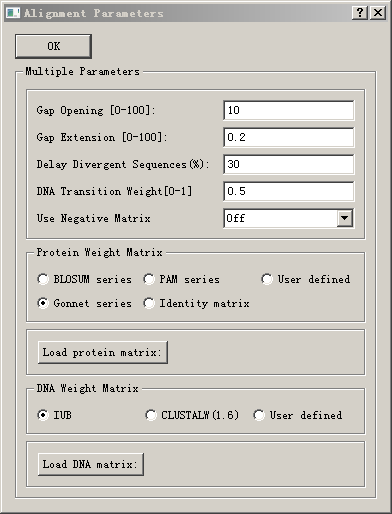
\includegraphics[width=0.5\textwidth]{P1}
    \caption{Pairwise \& Multiple Alignment Parameters for Clustal X}
    \label{P-01}
\end{figure}

\begin{figure}[H]
    \centering
    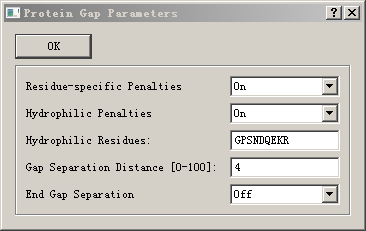
\includegraphics[width=0.5\textwidth]{P2}
    \caption{Protein Gap Parameters for Clustal X}
    \label{P-02}
\end{figure}


The parameters are basically default parameters, which works well. Increment of penalty for gap opening or extension gives out wired results with long gaps or scattered gaps.

To make the report brief, we show a part of the MSA results using Clustal X.

\begin{figure}[H]
    \centering
    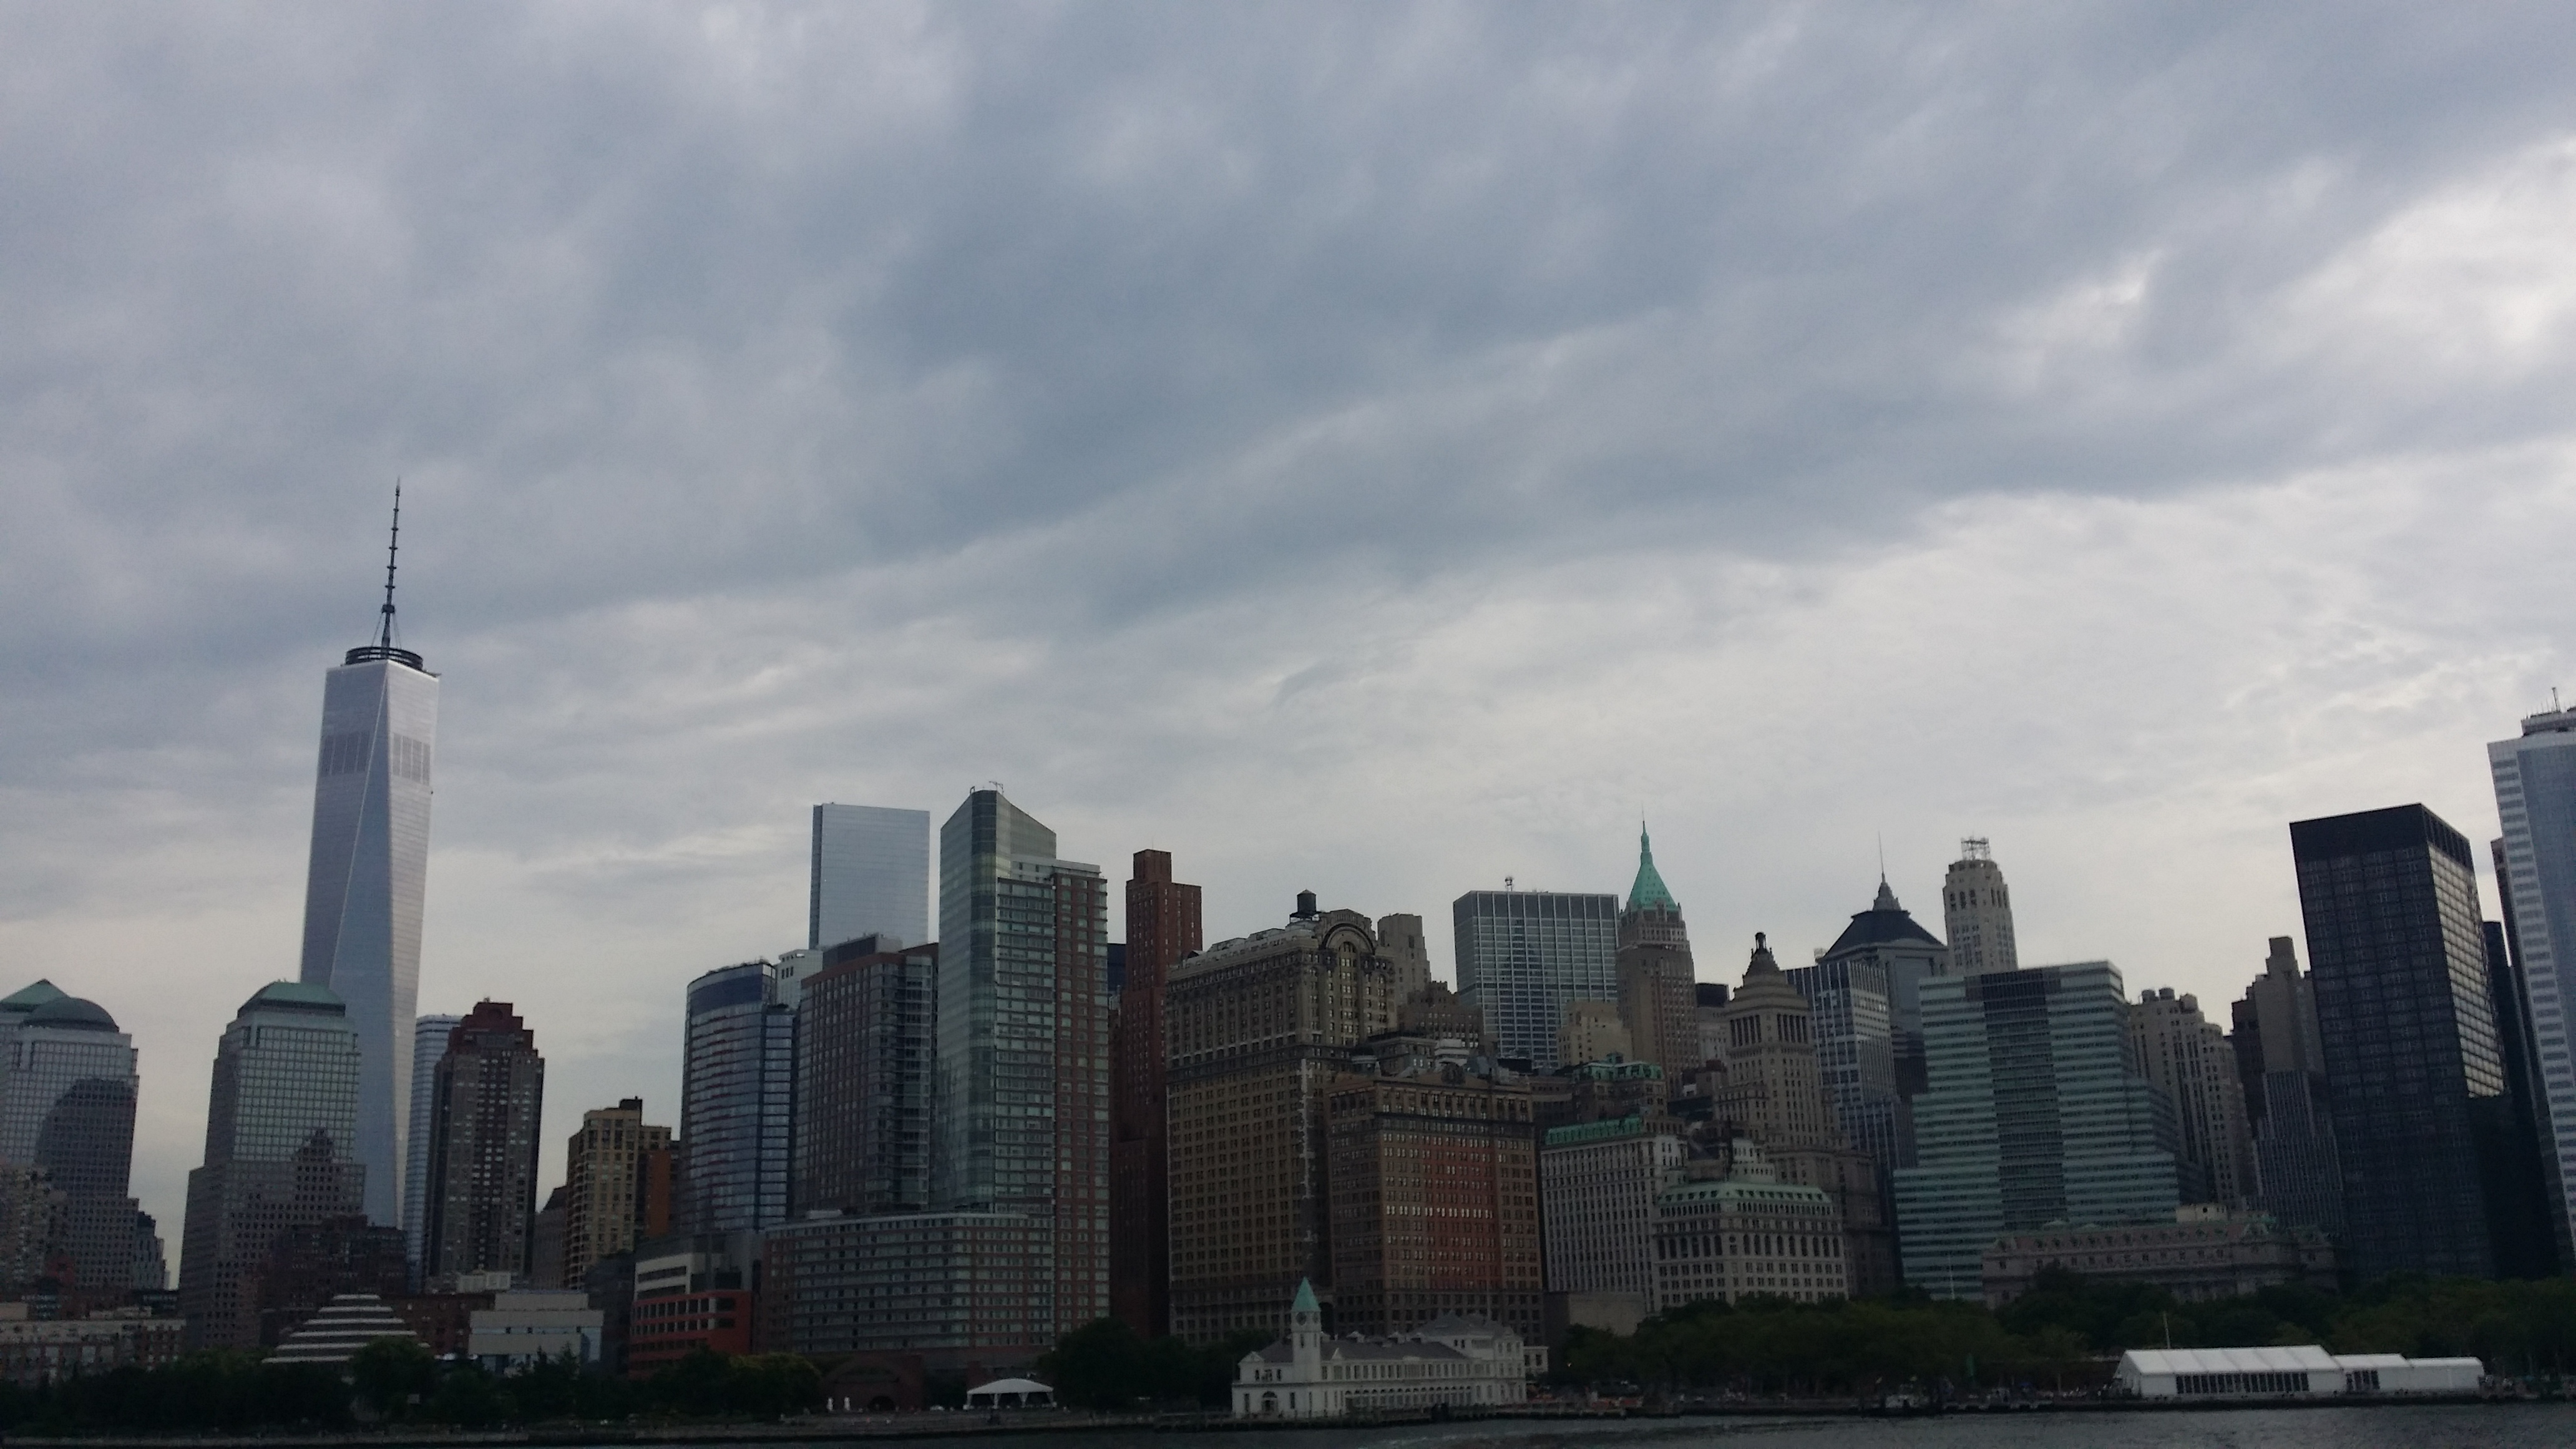
\includegraphics[width=1\textwidth]{F1}
    \caption{Part of MSA Results of Dataset 1 by Clustal X}
    \label{F-01}
\end{figure}

\subsubsection{Dataset 2}

We tried the tools like MUSCLE\upcite{edgar2004muscle}, Clustal W\upcite{larkin2007clustal} (packed in MegaX\upcite{kumar2018mega}), Clustal X\upcite{larkin2007clustal}, etc. and they gave out similar results under same parameters. 

The parameters are basically default parameters same as that used in dataset 1, which works well under the data set. Changing parameters have little, if any, impact on the results, with this dataset.

To make the report brief, we show a part of the MSA results using Clustal X.

\begin{figure}[H]
    \centering
    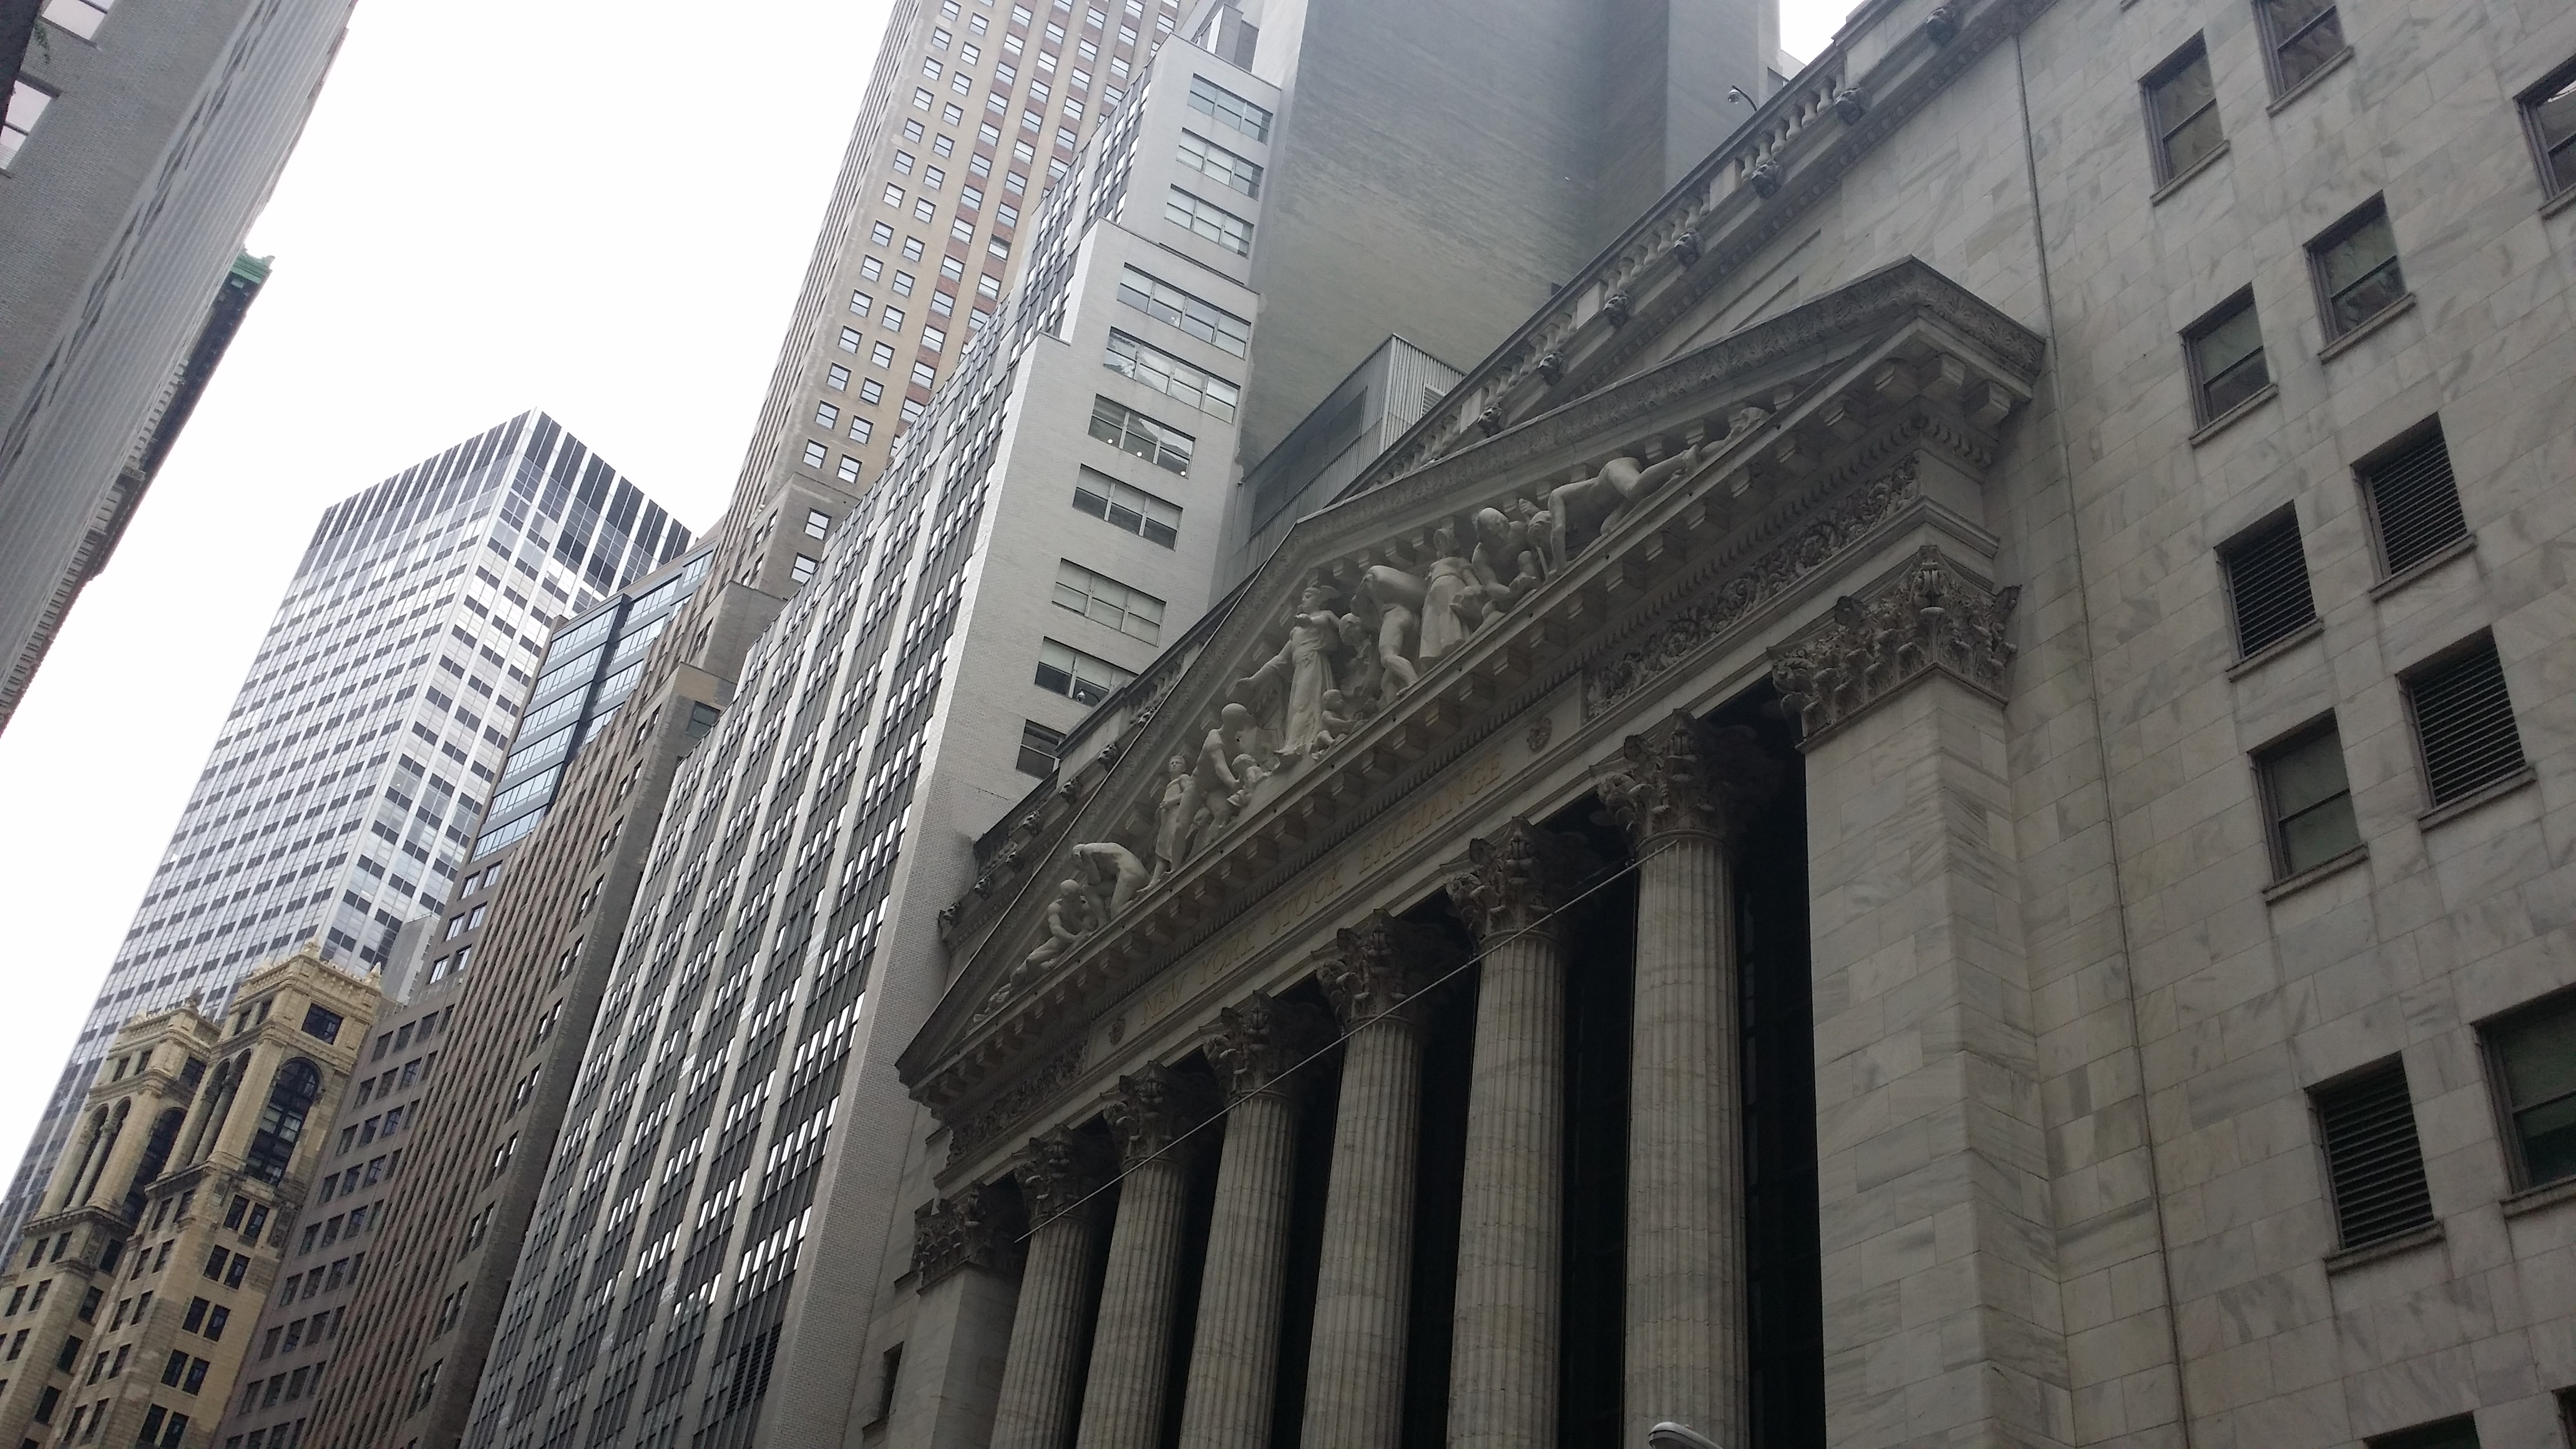
\includegraphics[width=1\textwidth]{F2}
    \caption{Part of MSA Results of Dataset 2 by Clustal X}
    \label{F-02}
\end{figure}


















\section{A defined receptor-binding domain (RBD) on S mediates the interaction of S with angiotensin converting enzyme 2 (ACE2). Are the regions conserved in your results?}

According to \citet{yan2020structural}, Spike glycoprotein in \textit{Severe acute respiratory syndrome coronavirus 2} have a receptor-binding domain (RBD) for angiotensin converting enzyme 2 (ACE2) within the \textbf{319 – 541} residues.\cite{yan2020structural}

MSA results of this domain is \textbf{significantly conserved} in the results of both data sets.



\subsubsection{Dataset 1}

The MSA results of conserved regions is shown in the figure below.
\begin{figure}[H]
    \centering
    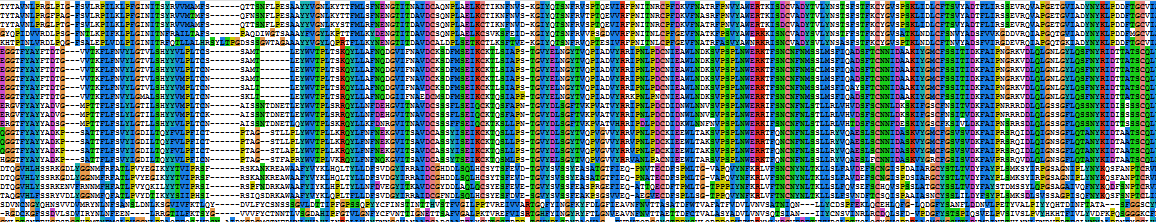
\includegraphics[width=1\textwidth]{S1}
    \caption{Conserved regions of the spike protein of SARS2-CoV as well as other coronavirus}
    \label{S-01}
\end{figure}

As is shown in the figure above, these sequences share some of the residues, but about one third of the residues have changed in the evolution.

\subsubsection{Dataset 2}

The MSA results of conserved regions is shown in the figure below.
\begin{figure}[H]
    \centering
    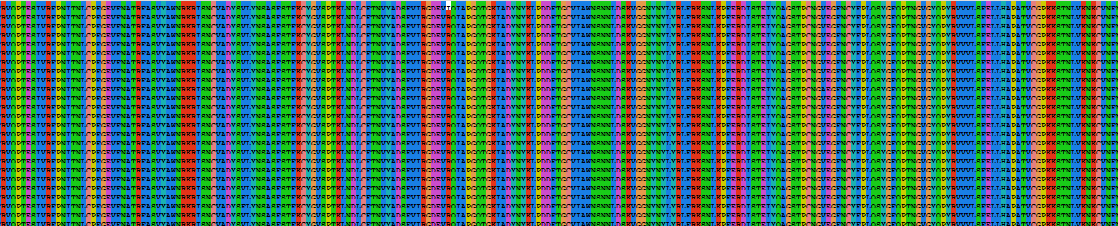
\includegraphics[width=1\textwidth]{S2}
    \caption{Conserved regions of the spike protein of different SARS2-CoV samples}
    \label{S-02}
\end{figure}

Different from the situation in Dataset 1, the results above indicates that most part of the region is identical in the samples, with only one residue changed in a sequence.


\section{Discussions}

Multiple sequence alignment is a powerful tool with many applications, such as creating a phylogenetic tree, identifying critical mutations, or finding conserved regions.

In many cases, the input set of query sequences are assumed to have an evolutionary relationship by which they share a linkage and are descended from a common ancestor. From the resulting MSA, sequence homology can be inferred and phylogenetic analysis can be conducted to assess the sequences' shared evolutionary origins.\upcite{wiki:Multiple_sequence_alignment}

The two datasets we select to demonstrate the multiple sequence alignment is more or less from the same origin, since sequences in Dataset 1 are from coronaviruses, and sequences in Dataset 1 are from the same virus but sampled in different times and places.

\subsection{Dataset 1}

The MSA results indicated several conserved regions. However, since are coronaviruses viruses with a positive-sense single-stranded RNA genome\upcite{cherry2013feigin}, their mutation rate tend to be high, and the conserved regions shares less features than those in eukaryotic cells.

As is shown above, even in in the family \textit{Coronaviridae}, the sequences of S protein can vary a lot, which allows us to identify the evolutionary relationship between different coronaviruses.

\begin{figure}[H]
    \centering
    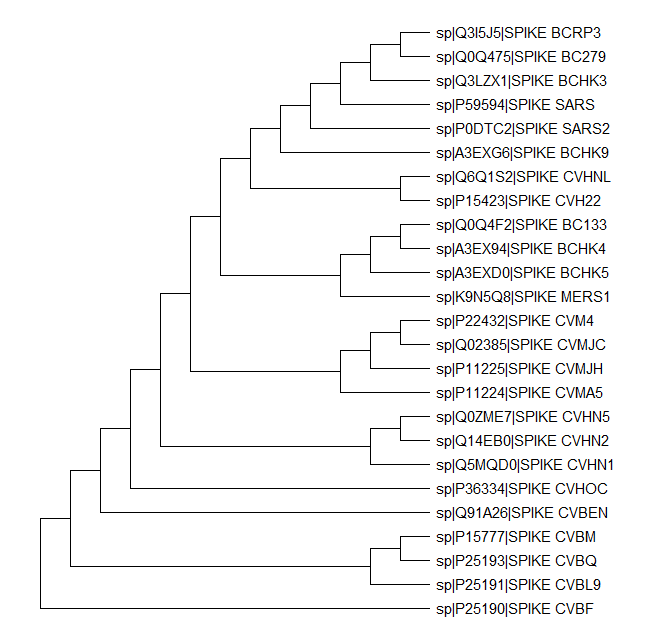
\includegraphics[width=1\textwidth]{T1}
    \caption{Phylogenetic Tree Generated by Dataset 1}
    \label{T-01}
\end{figure}


\subsubsection{Dataset 2}

The MSA results indicated several mutations, while most of the mutations seems to be minor mutations, such as the transformation of V to A. The different samples share most of the residues, but the small mutations can still help us to predict the time when the virus spreads to a specific country by using phylogenetic analysis based on the MSA results.

\begin{figure}[H]
    \centering
    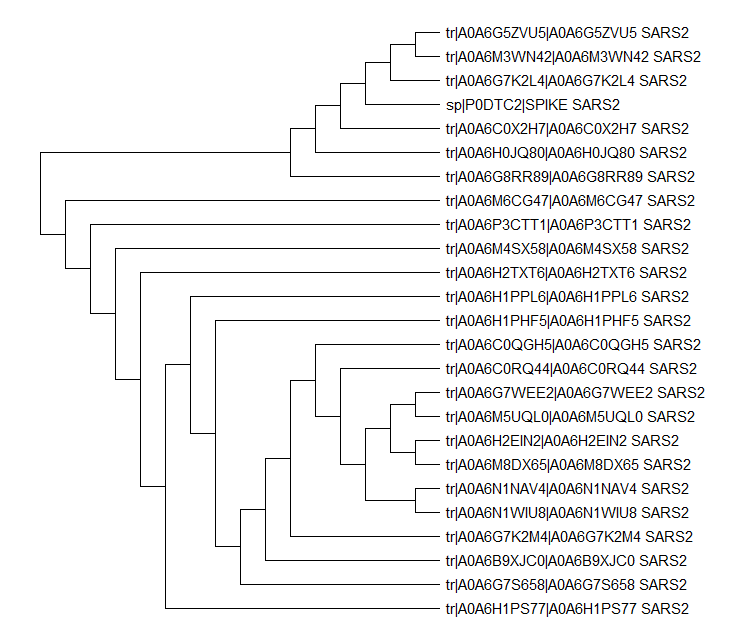
\includegraphics[width=1\textwidth]{T2}
    \caption{Phylogenetic Tree Generated by Dataset 2}
    \label{T-02}
\end{figure}



\section{Supplementary materials}



\subsection{Environment of this experiment}
The hardware we used is a x86\_64 compatible machine,
and the software used in the experiment is shown in the table below.

\begin{table}[H]
    \caption{Software used in the experiment}
    \centering
    \begin{tabular}{cc}
        \toprule
        Name&Version\\
        \midrule
        OS: Windows 10 Pro&20H2\\
        MegaX&10.1.7\\
        ClustalX&2.1\\
        \bottomrule
    \end{tabular}
\end{table}

\subsection{Dataset 1 fasta file}
\lstset{basicstyle=\tiny\ttfamily}
\begin{lstlisting}
>sp|P36334|SPIKE_CVHOC Spike glycoprotein OS=Human coronavirus OC43 OX=31631 GN=S PE=3 SV=1
MFLILLISLPTAFAVIGDLKCTSDNINDKDTGPPPISTDTVDVTNGLGTYYVLDRVYLNT
TLFLNGYYPTSGSTYRNMALKGSVLLSRLWFKPPFLSDFINGIFAKVKNTKVIKDRVMYS
EFPAITIGSTFVNTSYSVVVQPRTINSTQDGDNKLQGLLEVSVCQYNMCEYPQTICHPNL
GNHRKELWHLDTGVVSCLYKRNFTYDVNADYLYFHFYQEGGTFYAYFTDTGVVTKFLFNV
YLGMALSHYYVMPLTCNSKLTLEYWVTPLTSRQYLLAFNQDGIIFNAEDCMSDFMSEIKC
KTQSIAPPTGVYELNGYTVQPIADVYRRKPNLPNCNIEAWLNDKSVPSPLNWERKTFSNC
NFNMSSLMSFIQADSFTCNNIDAAKIYGMCFSSITIDKFAIPNGRKVDLQLGNLGYLQSF
NYRIDTTATSCQLYYNLPAANVSVSRFNPSTWNKRFGFIEDSVFKPRPAGVLTNHDVVYA
QHCFKAPKNFCPCKLNGSCVGSGPGKNNGIGTCPAGTNYLTCDNLCTPDPITFTGTYKCP
QTKSLVGIGEHCSGLAVKSDYCGGNSCTCRPQAFLGWSADSCLQGDKCNIFANFILHDVN
SGLTCSTDLQKANTDIILGVCVNYDLYGILGQGIFVEVNATYYNSWQNLLYDSNGNLYGF
RDYIINRTFMIRSCYSGRVSAAFHANSSEPALLFRNIKCNYVFNNSLTRQLQPINYFDSY
LGCVVNAYNSTAISVQTCDLTVGSGYCVDYSKNRRSRGAITTGYRFTNFEPFTVNSVNDS
LEPVGGLYEIQIPSEFTIGNMVEFIQTSSPKVTIDCAAFVCGDYAACKSQLVEYGSFCDN
INAILTEVNELLDTTQLQVANSLMNGVTLSTKLKDGVNFNVDDINFSPVLGCLGSECSKA
SSRSAIEDLLFDKVKLSDVGFVEAYNNCTGGAEIRDLICVQSYKGIKVLPPLLSENQISG
YTLAATSASLFPPWTAAAGVPFYLNVQYRINGLGVTMDVLSQNQKLIANAFNNALYAIQE
GFDATNSALVKIQAVVNANAEALNNLLQQLSNRFGAISASLQEILSRLDALEAEAQIDRL
INGRLTALNAYVSQQLSDSTLVKFSAAQAMEKVNECVKSQSSRINFCGNGNHIISLVQNA
PYGLYFIHFSYVPTKYVTARVSPGLCIAGDRGIAPKSGYFVNVNNTWMYTGSGYYYPEPI
TENNVVVMSTCAVNYTKAPYVMLNTSIPNLPDFKEELDQWFKNQTSVAPDLSLDYINVTF
LDLQVEMNRLQEAIKVLNQSYINLKDIGTYEYYVKWPWYVWLLICLAGVAMLVLLFFICC
CTGCGTSCFKKCGGCCDDYTGYQELVIKTSHDD
>sp|P0DTC2|SPIKE_SARS2 Spike glycoprotein OS=Severe acute respiratory syndrome coronavirus 2 OX=2697049 GN=S PE=1 SV=1
MFVFLVLLPLVSSQCVNLTTRTQLPPAYTNSFTRGVYYPDKVFRSSVLHSTQDLFLPFFS
NVTWFHAIHVSGTNGTKRFDNPVLPFNDGVYFASTEKSNIIRGWIFGTTLDSKTQSLLIV
NNATNVVIKVCEFQFCNDPFLGVYYHKNNKSWMESEFRVYSSANNCTFEYVSQPFLMDLE
GKQGNFKNLREFVFKNIDGYFKIYSKHTPINLVRDLPQGFSALEPLVDLPIGINITRFQT
LLALHRSYLTPGDSSSGWTAGAAAYYVGYLQPRTFLLKYNENGTITDAVDCALDPLSETK
CTLKSFTVEKGIYQTSNFRVQPTESIVRFPNITNLCPFGEVFNATRFASVYAWNRKRISN
CVADYSVLYNSASFSTFKCYGVSPTKLNDLCFTNVYADSFVIRGDEVRQIAPGQTGKIAD
YNYKLPDDFTGCVIAWNSNNLDSKVGGNYNYLYRLFRKSNLKPFERDISTEIYQAGSTPC
NGVEGFNCYFPLQSYGFQPTNGVGYQPYRVVVLSFELLHAPATVCGPKKSTNLVKNKCVN
FNFNGLTGTGVLTESNKKFLPFQQFGRDIADTTDAVRDPQTLEILDITPCSFGGVSVITP
GTNTSNQVAVLYQDVNCTEVPVAIHADQLTPTWRVYSTGSNVFQTRAGCLIGAEHVNNSY
ECDIPIGAGICASYQTQTNSPRRARSVASQSIIAYTMSLGAENSVAYSNNSIAIPTNFTI
SVTTEILPVSMTKTSVDCTMYICGDSTECSNLLLQYGSFCTQLNRALTGIAVEQDKNTQE
VFAQVKQIYKTPPIKDFGGFNFSQILPDPSKPSKRSFIEDLLFNKVTLADAGFIKQYGDC
LGDIAARDLICAQKFNGLTVLPPLLTDEMIAQYTSALLAGTITSGWTFGAGAALQIPFAM
QMAYRFNGIGVTQNVLYENQKLIANQFNSAIGKIQDSLSSTASALGKLQDVVNQNAQALN
TLVKQLSSNFGAISSVLNDILSRLDKVEAEVQIDRLITGRLQSLQTYVTQQLIRAAEIRA
SANLAATKMSECVLGQSKRVDFCGKGYHLMSFPQSAPHGVVFLHVTYVPAQEKNFTTAPA
ICHDGKAHFPREGVFVSNGTHWFVTQRNFYEPQIITTDNTFVSGNCDVVIGIVNNTVYDP
LQPELDSFKEELDKYFKNHTSPDVDLGDISGINASVVNIQKEIDRLNEVAKNLNESLIDL
QELGKYEQYIKWPWYIWLGFIAGLIAIVMVTIMLCCMTSCCSCLKGCCSCGSCCKFDEDD
SEPVLKGVKLHYT
>sp|Q6Q1S2|SPIKE_CVHNL Spike glycoprotein OS=Human coronavirus NL63 OX=277944 GN=S PE=1 SV=1
MKLFLILLVLPLASCFFTCNSNANLSMLQLGVPDNSSTIVTGLLPTHWFCANQSTSVYSA
NGFFYIDVGNHRSAFALHTGYYDANQYYIYVTNEIGLNASVTLKICKFSRNTTFDFLSNA
SSSFDCIVNLLFTEQLGAPLGITISGETVRLHLYNVTRTFYVPAAYKLTKLSVKCYFNYS
CVFSVVNATVTVNVTTHNGRVVNYTVCDDCNGYTDNIFSVQQDGRIPNGFPFNNWFLLTN
GSTLVDGVSRLYQPLRLTCLWPVPGLKSSTGFVYFNATGSDVNCNGYQHNSVVDVMRYNL
NFSANSLDNLKSGVIVFKTLQYDVLFYCSNSSSGVLDTTIPFGPSSQPYYCFINSTINTT
HVSTFVGILPPTVREIVVARTGQFYINGFKYFDLGFIEAVNFNVTTASATDFWTVAFATF
VDVLVNVSATNIQNLLYCDSPFEKLQCEHLQFGLQDGFYSANFLDDNVLPETYVALPIYY
QHTDINFTATASFGGSCYVCKPHQVNISLNGNTSVCVRTSHFSIRYIYNRVKSGSPGDSS
WHIYLKSGTCPFSFSKLNNFQKFKTICFSTVEVPGSCNFPLEATWHYTSYTIVGALYVTW
SEGNSITGVPYPVSGIREFSNLVLNNCTKYNIYDYVGTGIIRSSNQSLAGGITYVSNSGN
LLGFKNVSTGNIFIVTPCNQPDQVAVYQQSIIGAMTAVNESRYGLQNLLQLPNFYYVSNG
GNNCTTAVMTYSNFGICADGSLIPVRPRNSSDNGISAIITANLSIPSNWTTSVQVEYLQI
TSTPIVVDCATYVCNGNPRCKNLLKQYTSACKTIEDALRLSAHLETNDVSSMLTFDSNAF
SLANVTSFGDYNLSSVLPQRNIRSSRIAGRSALEDLLFSKVVTSGLGTVDVDYKSCTKGL
SIADLACAQYYNGIMVLPGVADAERMAMYTGSLIGGMVLGGLTSAAAIPFSLALQARLNY
VALQTDVLQENQKILAASFNKAINNIVASFSSVNDAITQTAEAIHTVTIALNKIQDVVNQ
QGSALNHLTSQLRHNFQAISNSIQAIYDRLDSIQADQQVDRLITGRLAALNAFVSQVLNK
YTEVRGSRRLAQQKINECVKSQSNRYGFCGNGTHIFSIVNSAPDGLLFLHTVLLPTDYKN
VKAWSGICVDGIYGYVLRQPNLVLYSDNGVFRVTSRVMFQPRLPVLSDFVQIYNCNVTFV
NISRVELHTVIPDYVDVNKTLQEFAQNLPKYVKPNFDLTPFNLTYLNLSSELKQLEAKTA
SLFQTTVELQGLIDQINSTYVDLKLLNRFENYIKWPWWVWLIISVVFVVLLSLLVFCCLS
TGCCGCCNCLTSSMRGCCDCGSTKLPYYEFEKVHVQ
>sp|K9N5Q8|SPIKE_MERS1 Spike glycoprotein OS=Middle East respiratory syndrome-related coronavirus (isolate United Kingdom/H123990006/2012) OX=1263720 GN=S PE=1 SV=1
MIHSVFLLMFLLTPTESYVDVGPDSVKSACIEVDIQQTFFDKTWPRPIDVSKADGIIYPQ
GRTYSNITITYQGLFPYQGDHGDMYVYSAGHATGTTPQKLFVANYSQDVKQFANGFVVRI
GAAANSTGTVIISPSTSATIRKIYPAFMLGSSVGNFSDGKMGRFFNHTLVLLPDGCGTLL
RAFYCILEPRSGNHCPAGNSYTSFATYHTPATDCSDGNYNRNASLNSFKEYFNLRNCTFM
YTYNITEDEILEWFGITQTAQGVHLFSSRYVDLYGGNMFQFATLPVYDTIKYYSIIPHSI
RSIQSDRKAWAAFYVYKLQPLTFLLDFSVDGYIRRAIDCGFNDLSQLHCSYESFDVESGV
YSVSSFEAKPSGSVVEQAEGVECDFSPLLSGTPPQVYNFKRLVFTNCNYNLTKLLSLFSV
NDFTCSQISPAAIASNCYSSLILDYFSYPLSMKSDLSVSSAGPISQFNYKQSFSNPTCLI
LATVPHNLTTITKPLKYSYINKCSRFLSDDRTEVPQLVNANQYSPCVSIVPSTVWEDGDY
YRKQLSPLEGGGWLVASGSTVAMTEQLQMGFGITVQYGTDTNSVCPKLEFANDTKIASQL
GNCVEYSLYGVSGRGVFQNCTAVGVRQQRFVYDAYQNLVGYYSDDGNYYCLRACVSVPVS
VIYDKETKTHATLFGSVACEHISSTMSQYSRSTRSMLKRRDSTYGPLQTPVGCVLGLVNS
SLFVEDCKLPLGQSLCALPDTPSTLTPRSVRSVPGEMRLASIAFNHPIQVDQLNSSYFKL
SIPTNFSFGVTQEYIQTTIQKVTVDCKQYVCNGFQKCEQLLREYGQFCSKINQALHGANL
RQDDSVRNLFASVKSSQSSPIIPGFGGDFNLTLLEPVSISTGSRSARSAIEDLLFDKVTI
ADPGYMQGYDDCMQQGPASARDLICAQYVAGYKVLPPLMDVNMEAAYTSSLLGSIAGVGW
TAGLSSFAAIPFAQSIFYRLNGVGITQQVLSENQKLIANKFNQALGAMQTGFTTTNEAFH
KVQDAVNNNAQALSKLASELSNTFGAISASIGDIIQRLDVLEQDAQIDRLINGRLTTLNA
FVAQQLVRSESAALSAQLAKDKVNECVKAQSKRSGFCGQGTHIVSFVVNAPNGLYFMHVG
YYPSNHIEVVSAYGLCDAANPTNCIAPVNGYFIKTNNTRIVDEWSYTGSSFYAPEPITSL
NTKYVAPQVTYQNISTNLPPPLLGNSTGIDFQDELDEFFKNVSTSIPNFGSLTQINTTLL
DLTYEMLSLQQVVKALNESYIDLKELGNYTYYNKWPWYIWLGFIAGLVALALCVFFILCC
TGCGTNCMGKLKCNRCCDRYEEYDLEPHKVHVH
>sp|P11224|SPIKE_CVMA5 Spike glycoprotein OS=Murine coronavirus (strain A59) OX=11142 GN=S PE=1 SV=2
MLFVFILFLPSCLGYIGDFRCIQLVNSNGANVSAPSISTETVEVSQGLGTYYVLDRVYLN
ATLLLTGYYPVDGSKFRNLALRGTNSVSLSWFQPPYLNQFNDGIFAKVQNLKTSTPSGAT
AYFPTIVIGSLFGYTSYTVVIEPYNGVIMASVCQYTICQLPYTDCKPNTNGNKLIGFWHT
DVKPPICVLKRNFTLNVNADAFYFHFYQHGGTFYAYYADKPSATTFLFSVYIGDILTQYY
VLPFICNPTAGSTFAPRYWVTPLVKRQYLFNFNQKGVITSAVDCASSYTSEIKCKTQSML
PSTGVYELSGYTVQPVGVVYRRVANLPACNIEEWLTARSVPSPLNWERKTFQNCNFNLSS
LLRYVQAESLFCNNIDASKVYGRCFGSISVDKFAVPRSRQVDLQLGNSGFLQTANYKIDT
AATSCQLHYTLPKNNVTINNHNPSSWNRRYGFNDAGVFGKNQHDVVYAQQCFTVRSSYCP
CAQPDIVSPCTTQTKPKSAFVNVGDHCEGLGVLEDNCGNADPHKGCICANNSFIGWSHDT
CLVNDRCQIFANILLNGINSGTTCSTDLQLPNTEVVTGICVKYDLYGITGQGVFKEVKAD
YYNSWQTLLYDVNGNLNGFRDLTTNKTYTIRSCYSGRVSAAFHKDAPEPALLYRNINCSY
VFSNNISREENPLNYFDSYLGCVVNADNRTDEALPNCDLRMGAGLCVDYSKSRRAHRSVS
TGYRLTTFEPYTPMLVNDSVQSVDGLYEMQIPTNFTIGHHEEFIQTRSPKVTIDCAAFVC
GDNTACRQQLVEYGSFCVNVNAILNEVNNLLDNMQLQVASALMQGVTISSRLPDGISGPI
DDINFSPLLGCIGSTCAEDGNGPSAIRGRSAIEDLLFDKVKLSDVGFVEAYNNCTGGQEV
RDLLCVQSFNGIKVLPPVLSESQISGYTTGATAAAMFPPWSAAAGVPFSLSVQYRINGLG
VTMNVLSENQKMIASAFNNALGAIQDGFDATNSALGKIQSVVNANAEALNNLLNQLSNRF
GAISASLQEILTRLEAVEAKAQIDRLINGRLTALNAYISKQLSDSTLIKVSAAQAIEKVN
ECVKSQTTRINFCGNGNHILSLVQNAPYGLYFIHFSYVPISFTTANVSPGLCISGDRGLA
PKAGYFVQDDGEWKFTGSSYYYPEPITDKNSVIMSSCAVNYTKAPEVFLNTSIPNPPDFK
EELDKWFKNQTSIAPDLSLDFEKLNVTLLDLTYEMNRIQDAIKKLNESYINLKEVGTYEM
YVKWPWYVWLLIGLAGVAVCVLLFFICCCTGCGSCCFKKCGNCCDEYGGHQDSIVIHNIS
SHED
>sp|P59594|SPIKE_SARS Spike glycoprotein OS=Severe acute respiratory syndrome coronavirus OX=694009 GN=S PE=1 SV=1
MFIFLLFLTLTSGSDLDRCTTFDDVQAPNYTQHTSSMRGVYYPDEIFRSDTLYLTQDLFL
PFYSNVTGFHTINHTFGNPVIPFKDGIYFAATEKSNVVRGWVFGSTMNNKSQSVIIINNS
TNVVIRACNFELCDNPFFAVSKPMGTQTHTMIFDNAFNCTFEYISDAFSLDVSEKSGNFK
HLREFVFKNKDGFLYVYKGYQPIDVVRDLPSGFNTLKPIFKLPLGINITNFRAILTAFSP
AQDIWGTSAAAYFVGYLKPTTFMLKYDENGTITDAVDCSQNPLAELKCSVKSFEIDKGIY
QTSNFRVVPSGDVVRFPNITNLCPFGEVFNATKFPSVYAWERKKISNCVADYSVLYNSTF
FSTFKCYGVSATKLNDLCFSNVYADSFVVKGDDVRQIAPGQTGVIADYNYKLPDDFMGCV
LAWNTRNIDATSTGNYNYKYRYLRHGKLRPFERDISNVPFSPDGKPCTPPALNCYWPLND
YGFYTTTGIGYQPYRVVVLSFELLNAPATVCGPKLSTDLIKNQCVNFNFNGLTGTGVLTP
SSKRFQPFQQFGRDVSDFTDSVRDPKTSEILDISPCSFGGVSVITPGTNASSEVAVLYQD
VNCTDVSTAIHADQLTPAWRIYSTGNNVFQTQAGCLIGAEHVDTSYECDIPIGAGICASY
HTVSLLRSTSQKSIVAYTMSLGADSSIAYSNNTIAIPTNFSISITTEVMPVSMAKTSVDC
NMYICGDSTECANLLLQYGSFCTQLNRALSGIAAEQDRNTREVFAQVKQMYKTPTLKYFG
GFNFSQILPDPLKPTKRSFIEDLLFNKVTLADAGFMKQYGECLGDINARDLICAQKFNGL
TVLPPLLTDDMIAAYTAALVSGTATAGWTFGAGAALQIPFAMQMAYRFNGIGVTQNVLYE
NQKQIANQFNKAISQIQESLTTTSTALGKLQDVVNQNAQALNTLVKQLSSNFGAISSVLN
DILSRLDKVEAEVQIDRLITGRLQSLQTYVTQQLIRAAEIRASANLAATKMSECVLGQSK
RVDFCGKGYHLMSFPQAAPHGVVFLHVTYVPSQERNFTTAPAICHEGKAYFPREGVFVFN
GTSWFITQRNFFSPQIITTDNTFVSGNCDVVIGIINNTVYDPLQPELDSFKEELDKYFKN
HTSPDVDLGDISGINASVVNIQKEIDRLNEVAKNLNESLIDLQELGKYEQYIKWPWYVWL
GFIAGLIAIVMVTILLCCMTSCCSCLKGACSCGSCCKFDEDDSEPVLKGVKLHYT
>sp|P15423|SPIKE_CVH22 Spike glycoprotein OS=Human coronavirus 229E OX=11137 GN=S PE=1 SV=1
MFVLLVAYALLHIAGCQTTNGLNTSYSVCNGCVGYSENVFAVESGGYIPSDFAFNNWFLL
TNTSSVVDGVVRSFQPLLLNCLWSVSGLRFTTGFVYFNGTGRGDCKGFSSDVLSDVIRYN
LNFEENLRRGTILFKTSYGVVVFYCTNNTLVSGDAHIPFGTVLGNFYCFVNTTIGNETTS
AFVGALPKTVREFVISRTGHFYINGYRYFTLGNVEAVNFNVTTAETTDFCTVALASYADV
LVNVSQTSIANIIYCNSVINRLRCDQLSFDVPDGFYSTSPIQSVELPVSIVSLPVYHKHT
FIVLYVDFKPQSGGGKCFNCYPAGVNITLANFNETKGPLCVDTSHFTTKYVAVYANVGRW
SASINTGNCPFSFGKVNNFVKFGSVCFSLKDIPGGCAMPIVANWAYSKYYTIGSLYVSWS
DGDGITGVPQPVEGVSSFMNVTLDKCTKYNIYDVSGVGVIRVSNDTFLNGITYTSTSGNL
LGFKDVTKGTIYSITPCNPPDQLVVYQQAVVGAMLSENFTSYGFSNVVELPKFFYASNGT
YNCTDAVLTYSSFGVCADGSIIAVQPRNVSYDSVSAIVTANLSIPSNWTTSVQVEYLQIT
STPIVVDCSTYVCNGNVRCVELLKQYTSACKTIEDALRNSARLESADVSEMLTFDKKAFT
LANVSSFGDYNLSSVIPSLPTSGSRVAGRSAIEDILFSKLVTSGLGTVDADYKKCTKGLS
IADLACAQYYNGIMVLPGVADAERMAMYTGSLIGGIALGGLTSAVSIPFSLAIQARLNYV
ALQTDVLQENQKILAASFNKAMTNIVDAFTGVNDAITQTSQALQTVATALNKIQDVVNQQ
GNSLNHLTSQLRQNFQAISSSIQAIYDRLDTIQADQQVDRLITGRLAALNVFVSHTLTKY
TEVRASRQLAQQKVNECVKSQSKRYGFCGNGTHIFSIVNAAPEGLVFLHTVLLPTQYKDV
EAWSGLCVDGTNGYVLRQPNLALYKEGNYYRITSRIMFEPRIPTMADFVQIENCNVTFVN
ISRSELQTIVPEYIDVNKTLQELSYKLPNYTVPDLVVEQYNQTILNLTSEISTLENKSAE
LNYTVQKLQTLIDNINSTLVDLKWLNRVETYIKWPWWVWLCISVVLIFVVSMLLLCCCST
GCCGFFSCFASSIRGCCESTKLPYYDVEKIHIQ
>sp|P22432|SPIKE_CVM4 Spike glycoprotein OS=Murine coronavirus (strain 4) OX=12760 GN=S PE=3 SV=1
MLFVFILLLPSCLGYIGDFRCIQTVNYNGNNASAPSISTEAVDVSKGLGTYYVLDRVYLN
ATLLLTGYYPVDGSNYRNLALTGTNTLSLTWFKPPFLSEFNDGIFAKVQNLKTNTPTGAT
SYFPTIVIGSLFGNTSYTVVLEPYNNIIMASVCTYTICQLPYTPCKPNTNGNRVIGFWHT
DVKPPICLLKRNFTFNVNAPWLYFHFYQQGGTFYAYYADKPSATTFLFSVYIGDILTQYF
VLPFICTPTAGSTLLPLYWVTPLLKRQYLFNFNEKGVITSAVDCASSYISEIKCKTQSLL
PSTGVYDLSGYTVQPVGVVYRRVPNLPDCKIEEWLTAKSVPSPLNWERRTFQNCNFNLSS
LLRYVQAESLSCNNIDASKVYGMCFGSVSVDKFAIPRSRQIDLQIGNSGFLQTANYKIDT
AATSCQLYYSLPKNNVTINNYNPSSWNRRYGFNDAGVFGKSKHDVAYAQQCFTVRPSYCP
CAQPDIVSACTSQTKPMSAYCPTGTIHRECSLWNGPHLRSARVGSGTYTCECTCKPNPFD
TYDLRCGQIKTIVNVGDHCEGLGVLEDKCGNSDPHKGCSCANDSFIGWSHDTCLVNDRCQ
IFANILLNGINSGTTCSTDLQLPNTEVATGVCVRYDLYGITGQGVFKEVKADYYNSWQAL
LYDVNGNLNGFRDLTTNKTYTIRSCYSGRVSAAYHKEAPEPALLYRNINCSYVFTNNISR
EENPLNYFDSYLGCVVNADNRTDEALPNCDLRMGAGLCVDYSKSRRARRSVSTGYRLTTF
EPYMPMLVNDSVQSVGGLYEMQIPTNFTIGHHEEFIQIRAPKVTIDCAAFVCGDNAACRQ
QLVEYGSFCDNVNAILNEVNNLLDNMQLQVASALMQGVTISSRLPDGISGPIDDINFSPL
LGCIGSTCAEDGNGPSAIRGRSAIEDLLFDKVKLSDVGFVEAYNNCTGGQEVRDLLCVQS
FNGIKVLPPVLSESQISGYTAGATAAAMFPPWTAAAGVPFSLNVQYRINGLGVTMNVLSE
NQKMIASAFNNALGAIQEGFDATNSALGKIQSVVNANAEALNNLLNQLSNRFGAISASLQ
EILTRLDAVEAKAQIDRLINGRLTALNAYISKQLSDSTLIKFSAAQAIEKVNECVKSQTT
RINFCGNGNHILSLVQNAPYGLCFIHFSYVPTSFKTANVSPGLCISGDRGLAPKAGYFVQ
DNGEWKFTGSNYYYPEPITDKNSVVMISCAVNYTKAPEVFLNNSIPNLPDFKEELDKWFK
NQTSIAPDLSLDFEKLNVTFLDLTYEMNRIQDAIKKLNESYINLKEVGTYEMYVKWPWYV
WLLIGLAGVAVCVLLFFICCCTGCGSCCFRKCGSCCDEYGGHQDSIVIHNISAHED
>sp|Q0ZME7|SPIKE_CVHN5 Spike glycoprotein OS=Human coronavirus HKU1 (isolate N5) OX=443241 GN=S PE=1 SV=1
MFLIIFILPTTLAVIGDFNCTNSFINDYNKTIPRISEDVVDVSLGLGTYYVLNRVYLNTT
LLFTGYFPKSGANFRDLALKGSIYLSTLWYKPPFLSDFNNGIFSKVKNTKLYVNNTLYSE
FSTIVIGSVFVNTSYTIVVQPHNGILEITACQYTMCEYPHTVCKSKGSIRNESWHIDSSE
PLCLFKKNFTYNVSADWLYFHFYQERGVFYAYYADVGMPTTFLFSLYLGTILSHYYVMPL
TCNAISSNTDNETLEYWVTPLSRRQYLLNFDEHGVITNAVDCSSSFLSEIQCKTQSFAPN
TGVYDLSGFTVKPVATVYRRIPNLPDCDIDNWLNNVSVPSPLNWERRIFSNCNFNLSTLL
RLVHVDSFSCNNLDKSKIFGSCFNSITVDKFAIPNRRRDDLQLGSSGFLQSSNYKIDISS
SSCQLYYSLPLVNVTINNFNPSSWNRRYGFGSFNLSSYDVVYSDHCFSVNSDFCPCADPS
VVNSCAKSKPPSAICPAGTKYRHCDLDTTLYVKNWCRCSCLPDPISTYSPNTCPQKKVVV
GIGEHCPGLGINEEKCGTQLNHSSCFCSPDAFLGWSFDSCISNNRCNIFSNFIFNGINSG
TTCSNDLLYSNTEISTGVCVNYDLYGITGQGIFKEVSAAYYNNWQNLLYDSNGNIIGFKD
FLTNKTYTILPCYSGRVSAAFYQNSSSPALLYRNLKCSYVLNNISFISQPFYFDSYLGCV
LNAVNLTSYSVSSCDLRMGSGFCIDYALPSSRRKRRGISSPYRFVTFEPFNVSFVNDSVE
TVGGLFEIQIPTNFTIAGHEEFIQTSSPKVTIDCSAFVCSNYAACHDLLSEYGTFCDNIN
SILNEVNDLLDITQLQVANALMQGVTLSSNLNTNLHSDVDNIDFKSLLGCLGSQCGSSSR
SLLEDLLFNKVKLSDVGFVEAYNNCTGGSEIRDLLCVQSFNGIKVLPPILSETQISGYTT
AATVAAMFPPWSAAAGVPFSLNVQYRINGLGVTMDVLNKNQKLIANAFNKALLSIQNGFT
ATNSALAKIQSVVNANAQALNSLLQQLFNKFGAISSSLQEILSRLDNLEAQVQIDRLING
RLTALNAYVSQQLSDITLIKAGASRAIEKVNECVKSQSPRINFCGNGNHILSLVQNAPYG
LLFIHFSYKPTSFKTVLVSPGLCLSGDRGIAPKQGYFIKQNDSWMFTGSSYYYPEPISDK
NVVFMNSCSVNFTKAPFIYLNNSIPNLSDFEAELSLWFKNHTSIAPNLTFNSHINATFLD
LYYEMNVIQESIKSLNSSFINLKEIGTYEMYVKWPWYIWLLIVILFIIFLMILFFICCCT
GCGSACFSKCHNCCDEYGGHNDFVIKASHDD
>sp|P11225|SPIKE_CVMJH Spike glycoprotein OS=Murine coronavirus (strain JHM) OX=11144 GN=S PE=1 SV=1
MLFVFILLLPSCLGYIGDFRCIQTVNYNGNNASAPSISTEAVDVSKGRGTYYVLDRVYLN
ATLLLTGYYPVDGSNYRNLALTGTNTLSLTWFKPPFLSEFNDGIFAKVQNLKTNTPTGAT
SYFPTIVIGSLFGNTSYTVVLEPYNNIIMASVCTYTICQLPYTPCKPNTNGNRVIGFWHT
DVKPPICLLKRNFTFNVNAPWLYFHFYQQGGTFYAYYADKPSATTFLFSVYIGDILTQYF
VLPFICTPTAGSTLAPLYWVTPLLKRQYLFNFNEKGVITSAVDCASSYISEIKCKTQSLL
PSTGVYDLSGYTVQPVGVVYRRVPNLPDCKIEEWLTAKSVPSPLNWERRTFQNCNFNLSS
LLRYVQAESLSCNNIDASKVYGMCFGSVSVDKFAIPRSRQIDLQIGNSGFLQTANYKIDT
AATSCQLYYSLPKNNVTINNYNPSSWNRRYGFKVNDRCQIFANILLNGINSGTTCSTDLQ
LPNTEVATGVCVRYDLYGITGQGVFKEVKADYYNSWQALLYDVNGNLNGFRDLTTNKTYT
IRSCYSGRVSAAYHKEAPEPALLYRNINCSYVFTNNISREENPLNYFDSYLGCVVNADNR
TDEALPNCNLRMGAGLCVDYSKSRRARRSVSTGYRLTTFEPYMPMLVNDSVQSVGGLYEM
QIPTNFTIGHHEEFIQIRAPKVTIDCAAFVCGDNAACRQQLVEYGSFCDNVNAILNEVNN
LLDNMQLQVASALMQGVTISSRLPDGISGPIDDINFSPLLGCIGSTCAEDGNGPSAIRGR
SAIEDLLFDKVKLSDVGFVEAYNNCTGGQEVRDLLCVQSFNGIKVLPPVLSESQISGYTA
GATAAAMFPPWTAAAGVPFSLNVQYRINGLGVTMNVLSENQKMIASAFNNALGAIQEGFD
ATNSALGKIQSVVNANAEALNNLLNQLSNRFGAISASLQEILTRLDAVEAKAQIDRLING
RLTALNAYISKQLSDSTLIKFSAAQAIEKVNECVKSQTTRINFCGNGNHILSLVQNAPYG
LCFIHFSYVPTSFKTANVSPGLCISGDRGLAPKAGYFVQDNGEWKFTGSNYYYPEPITDK
NSVAMISCAVNYTKAPEVFLNNSIPNLPDFKEELDKWFKNQTSIAPDLSLDFEKLNVTFL
DLTYEMNRIQDAIKKLNESYINLKEVGTYEMYVKWPWYVWLLIGLAGVAVCVLLFFICCC
TGCGSCCFRKCGSCCDEYGGHQDSIVIHNISAHED
>sp|Q02385|SPIKE_CVMJC Spike glycoprotein OS=Murine coronavirus (strain JHMV / variant CL-2) OX=33735 GN=S PE=1 SV=1
MLFVFILFLPSCLGYIGDFRCIQTVNYNGNNASAPSISTEAVDVSKGLGTYYVLDRVYLN
ATLLLTGYYPVDGSNYRNLALTGTNTLSLTWFKPPFLSEFNDGIFAKVQNLKTNTPTGAT
SYFPTIVIGSLFGNTSYTVVLEPYNNIIMASVCTYTICQLPYTPCKPNTNGNRVIGFWHT
DVKPPICLLKRNFTFNVNAPWLYFHFYQQGGTFYAYYADKPSATTFLFSVYIGDILTQYF
VLPFICTPTAGSTLLPLYWVTPLLKRQYLFNFNEKGVITSAVDCASSYISEIKCKTQSLL
PSTGVYDLSGYTVQPVGVVYRRVPNLPDCKIEEWLTAKSVPSPLNWERRTFQNCNFNLSS
LLRYVQAESLSCNNIDASKVYGMCFGSVSVDKFAIPRSRQIDLQIGNSGFLQTANYKIDT
AATSCQLYYSLPKNNVTINNYNPSSWNRRYGFNDAGVFGKSKHDVAYAQQCFIVRPSYCP
CAQPDIVSACTSQTKPMSAYCPTGTIHRECSLWNGPHLRSARVGSGTYTCECTCKPNPFD
TYDLRCGQIKTIVNVGDHCEGLGVLEDKCGNSDPHKGCSCAHDSFIGWSHDTCLVNDHSQ
IFANILLNGINSGTTCSTDLQLPNTEVATGVCVRYDLYGITGQGVFKEVKADYYNSWQAL
LYDVNGNLNGFRDLTTNKTYTIRSCYSGRVSAAYHKEAPEPALLYRNINCSYVFTNNISR
EENPLNYFDSYLGCVVNADNRPDEALPNCDLRMGAGLCVDYSKSRRARRSVSTGYRLTTF
EPYMPMLVNDSVQSVGGLYEMQIPTNFTIGHHEEFIQIRAPKVTIDCAAFVCGDNAACRQ
QLVEYGSFCDNVNAILNEVNNLLDNMQLQVASALMQGVTISSRLPDGISGPIDDINFSPL
LGCIGSTCAEDGNGPSAMRGRSAIEDLLFDKVKLSDVGFVEAYNNCTGGQEVRDLLCVQS
FNGIKVLPPVLSESQISGYTAGATAAAMFPPWTAAAGVPFSLNVQYRINGLGVTMNVLSE
NQKMIASAFNNALGAIQEGFDATNSALGKIQSVVNANAEALNNLLNQLSNRFGAISASLQ
EILTRLDRVEAKAQIDRLINGRLTALNAYISKQLSDSTLIKFSAAQAIEKVNECVKSQTT
RINFCGNGNHILSLVQNAPYGLCFIHFSYVPTSFKTANVSPGLCISGDRGLAPKAGYFVQ
DNGEWKFTGSNYYYPEPITDKNSVVMISCAVNYTKAPEVFLNNSIPNLPDFKEELDKWFK
NQTSIAPDLSLDFEKLNVTFLDLTYEMNRIQDAIKKLNESYINLKEVGTYEMYVKWPWYV
WLLIGLAGVAVCVLLFFICCCTGCGSCCFRKCGSCCDEYGGHQDSIVIYNISAHED
>sp|Q3I5J5|SPIKE_BCRP3 Spike glycoprotein OS=Bat coronavirus Rp3/2004 OX=349344 GN=S PE=1 SV=1
MKILILAFLASLAKAQEGCGIISRKPQPKMAQVSSSRRGVYYNDDIFRSNVLHLTQDYFL
PFDSNLTQYFSLNVDSDRFTYFDNPILDFGDGVYFAATEKSNVIRGWIFGSTFDNTTQSA
VIVNNSTHIIIRVCNFNLCKEPMYTVSRGAQQSSWVYQSAFNCTYDRVEKSFQLDTAPKT
GNFKDLREYVFKNRDGFLSVYQTYTAVNLPRGLPIGFSVLRPILKLPFGINITSYRVVMA
MFSQTTSNFLPESAAYYVGNLKYTTFMLSFNENGTITNAIDCAQNPLAELKCTIKNFNVS
KGIYQTSNFRVSPTQEVIRFPNITNRCPFDKVFNATRFPNVYAWERTKISDCVADYTVLY
NSTSFSTFKCYGVSPSKLIDLCFTSVYADTFLIRSSEVRQVAPGETGVIADYNYKLPDDF
TGCVIAWNTAKQDQGQYYYRSHRKTKLKPFERDLSSDENGVRTLSTYDFYPSVPVAYQAT
RVVVLSFELLNAPATVCGPKLSTQLVKNQCVNFNFNGLKGTGVLTESSKRFQSFQQFGRD
TSDFTDSVRDPQTLEILDISPCSFGGVSVITPGTNASSEVAVLYQDVNCTDVPAAIHADQ
LTPAWRVYSTGTNVFQTQAGCLIGAEHVNASYECDIPIGAGICASYHTASTLRSVGQKSI
VAYTMSLGAENSIAYANNSIAIPTNFSISVTTEVMPVSMAKTSVDCTMYICGDSLECSNL
LLQYGSFCTQLNRALSGIAIEQDKNTQEVFAQVKQMYKTPAIKDFGGFNFSQILPDPSKP
TKRSFIEDLLFNKVTLADAGFMKQYGECLGDISARDLICAQKFNGLTVLPPLLTDEMIAA
YTAALVSGTATAGWTFGAGSALQIPFAMQMAYRFNGIGVTQNVLYENQKQIANQFNKAIS
QIQESLTTTSTALGKLQDVVNQNAQALNTLVKQLSSNFGAISSVLNDILSRLDKVEAEVQ
IDRLITGRLQSLQTYVTQQLIRAAEIRASANLAATKMSECVLGQSKRVDFCGKGYHLMSF
PQAAPHGVVFLHVTYVPSQERNFTTAPAICHEGKAYFPREGVFVSNGTSWFITQRNFYSP
QIITTDNTFVAGSCDVVIGIINNTVYDPLQPELDSFKEELDKYFKNHTSPDVDLGDISGI
NASVVNIQKEIDRLNEVAKNLNESLIDLQELGKYEQYIKWPWYVWLGFIAGLIAIVMVTI
LLCCMTSCCSCLKGACSCGSCCKFDEDDSEPVLKGVKLHYT
>sp|Q5MQD0|SPIKE_CVHN1 Spike glycoprotein OS=Human coronavirus HKU1 (isolate N1) OX=443239 GN=S PE=1 SV=1
MLLIIFILPTTLAVIGDFNCTNFAINDLNTTVPRISEYVVDVSYGLGTYYILDRVYLNTT
ILFTGYFPKSGANFRDLSLKGTTYLSTLWYQKPFLSDFNNGIFSRVKNTKLYVNKTLYSE
FSTIVIGSVFINNSYTIVVQPHNGVLEITACQYTMCEYPHTICKSKGSSRNESWHFDKSE
PLCLFKKNFTYNVSTDWLYFHFYQERGTFYAYYADSGMPTTFLFSLYLGTLLSHYYVLPL
TCNAISSNTDNETLQYWVTPLSKRQYLLKFDNRGVITNAVDCSSSFFSEIQCKTKSLLPN
TGVYDLSGFTVKPVATVHRRIPDLPDCDIDKWLNNFNVPSPLNWERKIFSNCNFNLSTLL
RLVHTDSFSCNNFDESKIYGSCFKSIVLDKFAIPNSRRSDLQLGSSGFLQSSNYKIDTTS
SSCQLYYSLPAINVTINNYNPSSWNRRYGFNNFNLSSHSVVYSRYCFSVNNTFCPCAKPS
FASSCKSHKPPSASCPIGTNYRSCESTTVLDHTDWCRCSCLPDPITAYDPRSCSQKKSLV
GVGEHCAGFGVDEEKCGVLDGSYNVSCLCSTDAFLGWSYDTCVSNNRCNIFSNFILNGIN
SGTTCSNDLLQPNTEVFTDVCVDYDLYGITGQGIFKEVSAVYYNSWQNLLYDSNGNIIGF
KDFVTNKTYNIFPCYAGRVSAAFHQNASSLALLYRNLKCSYVLNNISLTTQPYFDSYLGC
VFNADNLTDYSVSSCALRMGSGFCVDYNSPSSSSSRRKRRSISASYRFVTFEPFNVSFVN
DSIESVGGLYEIKIPTNFTIVGQEEFIQTNSPKVTIDCSLFVCSNYAACHDLLSEYGTFC
DNINSILDEVNGLLDTTQLHVADTLMQGVTLSSNLNTNLHFDVDNINFKSLVGCLGPHCG
SSSRSFFEDLLFDKVKLSDVGFVEAYNNCTGGSEIRDLLCVQSFNGIKVLPPILSESQIS
GYTTAATVAAMFPPWSAAAGIPFSLNVQYRINGLGVTMDVLNKNQKLIATAFNNALLSIQ
NGFSATNSALAKIQSVVNSNAQALNSLLQQLFNKFGAISSSLQEILSRLDALEAQVQIDR
LINGRLTALNAYVSQQLSDISLVKFGAALAMEKVNECVKSQSPRINFCGNGNHILSLVQN
APYGLLFMHFSYKPISFKTVLVSPGLCISGDVGIAPKQGYFIKHNDHWMFTGSSYYYPEP
ISDKNVVFMNTCSVNFTKAPLVYLNHSVPKLSDFESELSHWFKNQTSIAPNLTLNLHTIN
ATFLDLYYEMNLIQESIKSLNNSYINLKDIGTYEMYVKWPWYVWLLISFSFIIFLVLLFF
ICCCTGCGSACFSKCHNCCDEYGGHHDFVIKTSHDD
>sp|P25191|SPIKE_CVBL9 Spike glycoprotein OS=Bovine coronavirus (strain L9) OX=11130 GN=S PE=1 SV=1
MFLILLISLPMAFAVIGDLKCTTVSINDVDTGAPSISTDIVDVTNGLGTYYVLDRVYLNT
TLLLNGYYPTSGSTYRNMALKGTLLLSRLWFKPPFLSDFINGIFAKVKNTKVIKKGVMYS
EFPAITIGSTFVNTSYSVVVQPHTTNLDNKLQGLLEISVCQYTMCEYPHTICHPNLGNKR
VELWHWDTGVVSCLYKRNFTYDVNADYLYFHFYQEGGTFYAYFTDTGVVTKFLFNVYLGT
VLSHYYVLPLTCNSAMTLEYWVTPLTSKQYLLAFNQDGVIFNAVDCKSDFMSEIKCKTLS
IAPSTGVYELNGYTVQPIADVYRRIPNLPDCNIEAWLNDKSVPSPLNWERKTFSNCNFNM
SCLMSFIQADSFTCNNIDAAKIYGMCFSSITIDKFAIPNGRKVDLQLGNLGYLQSFNYRI
DTTATSCQLYYNLPAANVSVSRFNPSTWNRRFGFTEQSVFKPQPVGVFTHHDVVYAQHCF
KAPTNFCPCKLDGSLCVGNGPGIDAGYKNSGIGTCPAGTNYLTCHNAAQCDCLCTPDPIT
SKSTGPYKCPQTKYLVGIGEHCSGLAIKSDYCGGNPCTCQPQAFLGWSVDSCLQGDRCNI
FANFILHDVNSGTTCSTDLQKSNTDIILGVCVNYDLYGITGQGIFVEVNAPYYNSWQNLL
YDSNGNLYGFRDYLTNRTFMIRSCYSGRVSAAFHANSSEPALLFRNIKCNYVFNNTLSRQ
LQPINYFDSYLGCVVNADNSTSSVVQTCDLTVGSGYCVDYSTKRRSRRAITTGYRFTNFE
PFTVNSVNDSLEPVGGLYEIQIPSEFTIGNMEEFIQTSSPKVTIDCSAFVCGDYAACKSQ
LVEYGSFCDNINAILTEVNELLDTTQLQVANSLMNGVTLSTKLKDGVNFNVDDINFSPVL
GCLGSDCNKVSSRSAIEDLLFSKVKLSDVGFVEAYNNCTGGAEIRDLICVQSYNGIKVLP
PLLSVNQISGYTLAATSASLFPPWSAAAGVPFYLNVQYRINGIGVTMDVLSQNQKLIANA
FNNALDAIQEGFDATNSALVKIQAVVNANAEALNNLLQQLSNRFGAISSSLQEILSRLDA
LEAQAQIDRLINGRLTALNAYVSQQLSDSTLVKFSAAQAMEKVNECVKSQSSRINFCGNG
NHIISLVQNAPYGLYFIHFSYVPTKYVTAKVSPGLCIAGDRGIAPKSGYFVNVNNTWMFT
GSGYYYPEPITGNNVVVMSTCAANYTKAPDVMLNISTPNLHDFKEELDQWFKNQTSVAPD
LSLDYINVTFLDLQDEMNRLQEAIKVLNQSYINLKDIGTYEYYVKWPWYVWLLIGFAGVA
MLVLLFFICCCTGCGTSCFKICGGCCDDYTGHQELVIKTSHDD
>sp|Q0Q4F2|SPIKE_BC133 Spike glycoprotein OS=Bat coronavirus 133/2005 OX=389230 GN=S PE=3 SV=1
MTRLMCLLMSLSIFVRGFDSQFVDMSPASNASECLESQVDAAAFSKLVWPYPIDPAKVDG
IIYPLGRTYSNITLEYTGLFPLQGDLGMQYLYSVSHAVGNDGDPTKAYISNYSLLVNDFD
NGFVVRIGAAANSTGTIVISPSVNTKIKKAYPAFILGSSLTNTSAGKPLYANYSLTIIPD
GCGTVLHAFYCILKPRTGNRCPSGSDYNAYFIYETIHSDCQSTINRNASLNSFKSFFDLV
NCTFFNSWDITADETKEWFGITQDTQGVHLHSSRKGDLYGGNMFRFATLPVYEGIKYYTV
IPRSFRSKANKREAWAAFYVYKLHQLTYLLDFSVDGYIRRAIDCGHDDLSQLHCSYTSFE
VDTGVYSVSSYEASATGTFIEQPNVTECDFSPMLTGVAPQVYNFKRLVFSNCNYNLTKLL
SLFAVDEFSCNGISPDAIARGCYSTLTVDYFAYPLSMKSYIRPGSAGNIPLYNYKQSFAN
PTCRVMASVPDNVTITKPGAYGYISKCSRLTGVNQDIETPLYINPGEYSICRDFAPLGFS
EDGQVFKRTLTQFEGGGLLIGVGTRVPMTANLEMGFVISVQYGTGTDSVCPMLDLGDSLT
ITNRLGKCVDYSLYGVTGRGVFQNCTAVGVKQQRFVYDSFDNLVGYYSDDGNYYCVRPCV
SVPVSVIYDKSTNLHATLFGSVACEHVTTMMSQFSRLTQSNLRRRDSNTPLQTAVGCVIG
LSNNSLVVSDCKLPLGQSLCAVPPVSMFRSYSASQFQLAVLNYTSPIVVTPINSSGFTAA
IPTNFSFSLTQEYIETSIQKVTVDCKQYVCNGFTRCEKLLVEYGQFCSKINQALHGANLR
QDESVYSLYSNIKTTSTQTLEYGLNGDFNLTLLQVPQIGGSSYRSAIEDLLFDKVTIADP
GYMQGYDDCMKQGPQSARDLICAQYVSGYKVLPPLYDPNMEAAYTSSLLGSIAGAGWTAG
LSSFAAIPFAQSMFYRLNGVGITQQVLSENQKLIANKFNQALGAMQTGFTTSNLAFSKVQ
DAVNANAQALSKLASELSNTFGAISSSISDILARLDTVEQDAQIDRLINGRLTSLNAFVS
QQLVRSETAARSAQLASDKVNECVKSQSKRNGFCGSGTHIVSFVVNAPNGFYFFHVGYVP
TNYTNVTAAYGLCNHNNPPLCIAPIDGYFITNQTTTYSVDTEWYYTGSSFFKPEPITQAN
SRYVSSDVKFEKLENNLPPPLLENSTDVDFKDELEEFFKNVTSHGPNFAEISKINTTLLD
LSDEMAILQEVVKQLNDSYIDLKELGNYTYYNKWPWYIWLGFIAGLVALLLCVFFLLCCT
GCGTSCLGKMKCKNCCDSYEEYDVEKIHVH
>sp|A3EXG6|SPIKE_BCHK9 Spike glycoprotein OS=Bat coronavirus HKU9 OX=694006 GN=S PE=1 SV=1
MLLILVLGVSLAAASRPECFNPRFTLTPLNHTLNYTSIKAKVSNVLLPDPYIAYSGQTLR
QNLFMADMSNTILYPVTPPANGANGGFIYNTSIIPVSAGLFVNTWMYRQPASSRAYCQEP
FGVAFGDTFENDRIAILIMAPDNLGSWSAVAPRNQTNIYLLVCSNATLCINPGFNRWGPA
GSFIAPDALVDHSNSCFVNNTFSVNISTSRISLAFLFKDGDLLIYHSGWLPTSNFEHGFS
RGSHPMTYFMSLPVGGNLPRAQFFQSIVRSNAIDKGDGMCTNFDVNLHVAHLINRDLLVS
YFNNGSVANAADCADSAAEELYCVTGSFDPPTGVYPLSRYRAQVAGFVRVTQRGSYCTPP
YSVLQDPPQPVVWRRYMLYDCVFDFTVVVDSLPTHQLQCYGVSPRRLASMCYGSVTLDVM
RINETHLNNLFNRVPDTFSLYNYALPDNFYGCLHAFYLNSTAPYAVANRFPIKPGGRQSN
SAFIDTVINAAHYSPFSYVYGLAVITLKPAAGSKLVCPVANDTVVITDRCVQYNLYGYTG
TGVLSKNTSLVIPDGKVFTASSTGTIIGVSINSTTYSIMPCVTVPVSVGYHPNFERALLF
NGLSCSQRSRAVTEPVSVLWSASATAQDAFDTPSGCVVNVELRNTTIVNTCAMPIGNSLC
FINGSIATANADSLPRLQLVNYDPLYDNSTATPMTPVYWVKVPTNFTLSATEEYIQTTAP
KITIDCARYLCGDSSRCLNVLLHYGTFCNDINKALSRVSTILDSALLSLVKELSINTRDE
VTTFSFDGDYNFTGLMGCLGPNCGATTYRSAFSDLLYDKVRITDPGFMQSYQKCIDSQWG
GSIRDLLCTQTYNGIAVLPPIVSPAMQALYTSLLVGAVASSGYTFGITSAGVIPFATQLQ
FRLNGIGVTTQVLVENQKLIASSFNNALVNIQKGFTETSIALSKMQDVINQHAAQLHTLV
VQLGNSFGAISSSINEIFSRLEGLAANAEVDRLINGRMMVLNTYVTQLLIQASEAKAQNA
LAAQKISECVKAQSLRNDFCGNGTHVLSIPQLAPNGVLFIHYAYTPTEYAFVQTSAGLCH
NGTGYAPRQGMFVLPNNTNMWHFTTMQFYNPVNISASNTQVLTSCSVNYTSVNYTVLEPS
VPGDYDFQKEFDKFYKNLSTIFNNTFNPNDFNFSTVDVTAQIKSLHDVVNQLNQSFIDLK
KLNVYEKTIKWPWYVWLAMIAGIVGLVLAVIMLMCMTNCCSCFKGMCDCRRCCGSYDSYD
DVYPAVRVNKKRTV
>sp|A3EXD0|SPIKE_BCHK5 Spike glycoprotein OS=Bat coronavirus HKU5 OX=694008 GN=S PE=1 SV=1
MIRSVLVLMCSLTFIGNLTRGQSVDMGHNGTGSCLDSQVQPDYFESVHTTWPMPIDTSKA
EGVIYPNGKSYSNITLTYTGLYPKANDLGKQYLFSDGHSAPGRLNNLFVSNYSSQVESFD
DGFVVRIGAAANKTGTTVISQSTFKPIKKIYPAFLLGHSVGNYTPSNRTGRYLNHTLVIL
PDGCGTILHAFYCVLHPRTQQNCAGETNFKSLSLWDTPASDCVSGSYNQEATLGAFKVYF
DLINCTFRYNYTITEDENAEWFGITQDTQGVHLYSSRKENVFRNNMFHFATLPVYQKILY
YTVIPRSIRSPFNDRKAWAAFYIYKLHPLTYLLNFDVEGYITKAVDCGYDDLAQLQCSYE
SFEVETGVYSVSSFEASPRGEFIEQATTQECDFTPMLTGTPPPIYNFKRLVFTNCNYNLT
KLLSLFQVSEFSCHQVSPSSLATGCYSSLTVDYFAYSTDMSSYLQPGSAGAIVQFNYKQD
FSNPTCRVLATVPQNLTTITKPSNYAYLTECYKTSAYGKNYLYNAPGAYTPCLSLASRGF
STKYQSHSDGELTTTGYIYPVTGNLQMAFIISVQYGTDTNSVCPMQALRNDTSIEDKLDV
CVEYSLHGITGRGVFHNCTSVGLRNQRFVYDTFDNLVGYHSDNGNYYCVRPCVSVPVSVI
YDKASNSHATLFGSVACSHVTTMMSQFSRMTKTNLLARTTPGPLQTTVGCAMGFINSSMV
VDECQLPLGQSLCAIPPTTSSRVRRATSGASDVFQIATLNFTSPLTLAPINSTGFVVAVP
TNFTFGVTQEFIETTIQKITVDCKQYVCNGFKKCEDLLKEYGQFCSKINQALHGANLRQD
ESIANLFSSIKTQNTQPLQAGLNGDFNLTMLQIPQVTTGERKYRSTIEDLLFNKVTIADP
GYMQGYDECMQQGPQSARDLICAQYVAGYKVLPPLYDPYMEAAYTSSLLGSIAGASWTAG
LSSFAAIPFAQSIFYRLNGVGITQQVLSENQKIIANKFNQALGAMQTGFTTTNLAFNKVQ
DAVNANAMALSKLAAELSNTFGAISSSISDILARLDTVEQEAQIDRLINGRLTSLNAFVA
QQLVRTEAAARSAQLAQDKVNECVKSQSKRNGFCGTGTHIVSFAINAPNGLYFFHVGYQP
TSHVNATAAYGLCNTENPQKCIAPIDGYFVLNQTTSTVADSDQQWYYTGSSFFHPEPITE
ANSKYVSMDVKFENLTNRLPPPLLSNSTDLDFKEELEEFFKNVSSQGPNFQEISKINTTL
LNLNTELMVLSEVVKQLNESYIDLKELGNYTFYQKWPWYIWLGFIAGLVALALCVFFILC
CTGCGTSCLGKLKCNRCCDSYDEYEVEKIHVH
>sp|A3EX94|SPIKE_BCHK4 Spike glycoprotein OS=Bat coronavirus HKU4 OX=694007 GN=S PE=1 SV=1
MTLLMCLLMSLLIFVRGCDSQFVDMSPASNTSECLESQVDAAAFSKLMWPYPIDPSKVDG
IIYPLGRTYSNITLAYTGLFPLQGDLGSQYLYSVSHAVGHDGDPTKAYISNYSLLVNDFD
NGFVVRIGAAANSTGTIVISPSVNTKIKKAYPAFILGSSLTNTSAGQPLYANYSLTIIPD
GCGTVLHAFYCILKPRTVNRCPSGTGYVSYFIYETVHNDCQSTINRNASLNSFKSFFDLV
NCTFFNSWDITADETKEWFGITQDTQGVHLYSSRKGDLYGGNMFRFATLPVYEGIKYYTV
IPRSFRSKANKREAWAAFYVYKLHQLTYLLDFSVDGYIRRAIDCGHDDLSQLHCSYTSFE
VDTGVYSVSSYEASATGTFIEQPNATECDFSPMLTGVAPQVYNFKRLVFSNCNYNLTKLL
SLFAVDEFSCNGISPDSIARGCYSTLTVDYFAYPLSMKSYIRPGSAGNIPLYNYKQSFAN
PTCRVMASVLANVTITKPHAYGYISKCSRLTGANQDVETPLYINPGEYSICRDFSPGGFS
EDGQVFKRTLTQFEGGGLLIGVGTRVPMTDNLQMSFIISVQYGTGTDSVCPMLDLGDSLT
ITNRLGKCVDYSLYGVTGRGVFQNCTAVGVKQQRFVYDSFDNLVGYYSDDGNYYCVRPCV
SVPVSVIYDKSTNLHATLFGSVACEHVTTMMSQFSRLTQSNLRRRDSNIPLQTAVGCVIG
LSNNSLVVSDCKLPLGQSLCAVPPVSTFRSYSASQFQLAVLNYTSPIVVTPINSSGFTAA
IPTNFSFSVTQEYIETSIQKVTVDCKQYVCNGFTRCEKLLVEYGQFCSKINQALHGANLR
QDESVYSLYSNIKTTSTQTLEYGLNGDFNLTLLQVPQIGGSSSSYRSAIEDLLFDKVTIA
DPGYMQGYDDCMKQGPQSARDLICAQYVSGYKVLPPLYDPNMEAAYTSSLLGSIAGAGWT
AGLSSFAAIPFAQSMFYRLNGVGITQQVLSENQKLIANKFNQALGAMQTGFTTSNLAFSK
VQDAVNANAQALSKLASELSNTFGAISSSISDILARLDTVEQDAQIDRLINGRLISLNAF
VSQQLVRSETAARSAQLASDKVNECVKSQSKRNGFCGSGTHIVSFVVNAPNGFYFFHVGY
VPTNYTNVTAAYGLCNNNNPPLCIAPIDGYFITNQTTTYSVDTEWYYTGSSFYKPEPITQ
ANSRYVSSDVKFDKLENNLPPPLLENSTDVDFKDELEEFFKNVTSHGPNFAEISKINTTL
LDLSDEMAMLQEVVKQLNDSYIDLKELGNYTYYNKWPWYVWLGFIAGLVALLLCVFFLLC
CTGCGTSCLGKMKCKNCCDSYEEYDVEKIHVH
>sp|Q3LZX1|SPIKE_BCHK3 Spike glycoprotein OS=Bat coronavirus HKU3 OX=442736 GN=S PE=3 SV=1
MKILIFAFLANLAKAQEGCGIISRKPQPKMAQVSSSRRGVYYNDDIFRSDVLHLTQDYFL
PFDSNLTQYFSLNVDSDRYTYFDNPILDFGDGVYFAATEKSNVIRGWIFGSSFDNTTQSA
VIVNNSTHIIIRVCNFNLCKEPMYTVSRGTQQNAWVYQSAFNCTYDRVEKSFQLDTTPKT
GNFKDLREYVFKNRDGFLSVYQTYTAVNLPRGLPTGFSVLKPILKLPFGINITSYRVVMA
MFSQTTSNFLPESAAYYVGNLKYSTFMLRFNENGTITDAVDCSQNPLAELKCTIKNFNVD
KGIYQTSNFRVSPTQEVIRFPNITNRCPFDKVFNATRFPNVYAWERTKISDCVADYTVLY
NSTSFSTFKCYGVSPSKLIDLCFTSVYADTFLIRSSEVRQVAPGETGVIADYNYKLPDDF
TGCVIAWNTAKHDTGNYYYRSHRKTKLKPFERDLSSDDGNGVYTLSTYDFNPNVPVAYQA
TRVVVLSFELLNAPATVCGPKLSTELVKNQCVNFNFNGLKGTGVLTSSSKRFQSFQQFGR
DTSDFTDSVRDPQTLEILDISPCSFGGVSVITPGTNASSEVAVLYQDVNCTDVPTAIRAD
QLTPAWRVYSTGVNVFQTQAGCLIGAEHVNASYECDIPIGAGICASYHTASVLRSTGQKS
IVAYTMSLGAENSIAYANNSIAIPTNFSISVTTEVMPVSMAKTAVDCTMYICGDSLECSN
LLLQYGSFCTQLNRALTGIAIEQDKNTQEVFAQVKQMYKTPAIKDFGGFNFSQILPDPSK
PTKRSFIEDLLFNKVTLADAGFMKQYGDCLGDVSARDLICAQKFNGLTVLPPLLTDEMVA
AYTAALVSGTATAGWTFGAGAALQIPFAMQMAYRFNGIGVTQNVLYENQKLIANQFNSAI
GKIQESLSSTASALGKLQDVVNQNAQALNTLVKQLSSNFGAISSVLNDILSRLDKVEAEV
QIDRLITGRLQSLQTYVTQQLIRAAEIRASANLAATKMSECVLGQSKRVDFCGKGYHLMS
FPQSAPHGVVFLHVTYVPSQEKNFTTAPAICHEGKAYFPREGVFVSNGTSWFITQRNFYS
PQLITTDNTFVSGNCDVVIGIINNTVYDPLQPELDSFKEELDKYFKNHTSPDVDLGDISG
INASVVNIQKEIDRLNEVAKNLNESLIDLQELGKYEQYIKWPWYVWLGFIAGLIAIVMVT
ILLCCMTSCCSCLKGACSCGSCCKFDEDDSEPVLKGVKLHYT
>sp|Q0Q475|SPIKE_BC279 Spike glycoprotein OS=Bat coronavirus 279/2005 OX=389167 GN=S PE=3 SV=1
MKVLIFALLFSLAKAQEGCGIISRKPQPKMEKVSSSRRGVYYNDDIFRSDVLHLTQDYFL
PFDSNLTQYFSLNIDSNKYTYFDNPILDFGDGVYFAATEKSNVIRGWIFGSSFDNTTQSA
IIVNNSTHIIIRVCNFNLCKEPMYTVSKGTQQSSWVYQSAFNCTYDRVEKSFQLDTAPKT
GNFKDLREYVFKNRDGFLSVYQTYTAVNLPRGFPAGFSVLRPILKLPFGINITSYRVVMT
MFSQFNSNFLPESAAYYVGNLKYTTFMLSFNENGTITDAVDCSQNPLAELKCTIKNFNVS
KGIYQTSNFRVTPTQEVVRFPNITNRCPFDKVFNASRFPNVYAWERTKISDCVADYTVLY
NSTSFSTFKCYGVSPSKLIDLCFTSVYADTFLIRSSEVRQVAPGETGVIADYNYKLPDDF
TGCVIAWNTAQQDQGQYYYRSYRKEKLKPFERDLSSDENGVYTLSTYDFYPSIPVEYQAT
RVVVLSFELLNAPATVCGPKLSTQLVKNQCVNFNFNGLRGTGVLTTSSKRFQSFQQFGRD
TSDFTDSVRDPQTLEILDISPCSFGGVSVITPGTNASSEVAVLYQDVNCTDVPTSIHADQ
LTPAWRVYSTGVNVFQTQAGCLIGAEHVNASYECDIPIGAGICASYHTASVLRSTGQKSI
VAYTMSLGAENSIAYANNSIAIPTNFSISVTTEVMPVSIAKTSVDCTMYICGDSLECSNL
LLQYGSFCTQLNRALTGIAIEQDKNTQEVFAQVKQMYKTPAIKDFGGFNFSQILPDPSKP
TKRSFIEDLLFNKVTLADAGFMKQYGECLGDISARDLICAQKFNGLTVLPPLLTDEMIAA
YTAALVSGTATAGWTFGAGSALQIPFAMQMAYRFNGIGVTQNVLYENQKQIANQFNKAIS
QIQESLTTTSTALGKLQDVVNDNAQALNTLVKQLSSNFGAISSVLNDILSRLDKVEAEVQ
IDRLITGRLQSLQTYVTQQLIRAAEIRASANLAATKMSECVLGQSKRVDFCGKGYHLMSF
PQAAPHGVVFLHVTYVPSQERNFTTAPAICHEGKAYFPREGVFVSNGTSWFITQRNFYSP
QIITTDNTFVAGNCDVVIGIINNTVYDPLQPELDSFKEELDKYFKNHTSPDVDLGDISGI
NASVVNIQKEIDRLNEVAKNLNESLIDLQELGKYEQYIKWPWYVWLGFIAGLIAIVMVTI
LLCCMTSCCSCLKGACSCGSCCKFDEDDSEPVLKGVKLHYT
>sp|Q14EB0|SPIKE_CVHN2 Spike glycoprotein OS=Human coronavirus HKU1 (isolate N2) OX=443240 GN=S PE=3 SV=1
MFLIIFILPTTLAVIGDFNCTNSFINDYNKTIPRISEDVVDVSLGLGTYYVLNRVYLNTT
LLFTGYFPKSGANFRDLALKGSKYLSTLWYKPPFLSDFNNGIFSKVKNTKLYVNNTLYSE
FSTIVIGSVFVNTSYTIVVQPHNGILEITACQYTMCEYPHTVCKSKGSIRNESWHIDSSE
PLCLFKKNFTYNVSADWLYFHFYQERGVFYAYYADVGMPTTFLFSLYLGTILSHYYVMPL
TCKAISSNTDNETLEYWVTPLSRRQYLLNFDEHGVITNAVDCSSSFLSEIQCKTQSFAPN
TGVYDLSGFTVKPVATVYRRIPNLPDCDIDNWLNNVSVPSPLNWERRIFSNCNFNLSTLL
RLVHVDSFSCNNLDKSKIFGSCFNSITVDKFAIPNRRRDDLQLGSSGFLQSSNYKIDISS
SSCQLYYSLPLVNVTINNFNPSSWNRRYGFGSFNVSSYDVVYSDHCFSVNSDFCPCADPS
VVNSCVKSKPLSAICPAGTKYRHCDLDTTLYVNNWCRCSCLPDPISTYSPNTCPQKKVVV
GIGEHCPGLGINEEKCGTQLNHSSCSCSPDAFLGWSFDSCISNNRCNIFSNFIFNGINSG
TTCSNDLLYSNTEVSTGVCVNYDLYGITGQGIFKEVSAAYYNNWQNLLYDSNGNIIGFKD
FLTNKTYTILPCYSGRVSAAFYQNSSSPALLYRNLKCSYVLNNISFISQPFYFDSYLGCV
LNAVNLTSYSVSSCDLRMGSGFCIDYALPSSRRKRRGISSPYRFVTFEPFNVSFVNDSVE
TVGGLFEIQIPTNFTIAGHEEFIQTSSPKVTIDCSAFVCSNYAACHDLLSEYGTFCDNIN
SILNEVNDLLDITQLQVANALMQGVTLSSNLNTNLHSDVDNIDFKSLLGCLGSQCGSSSR
SLLEDLLFNKVKLSDVGFVEAYNNCTGGSEIRDLLCVQSFNGIKVLPPILSETQISGYTT
AATVAAMFPPWSAAAGVPFSLNVQYRINGLGVTMDVLNKNQKLIANAFNKALLSIQNGFT
ATNSALAKIQSVVNANAQALNSLLQQLFNKFGAISSSLQEILSRLDNLEAQVQIDRLING
RLTALNAYVSQQLSDITLIKAGASRAIEKVNECVKSQSPRINFCGNGNHILSLVQNAPYG
LLFIHFSYKPTSFKTVLVSPGLCLSGDRGIAPKQGYFIKQNDSWMFTGSSYYYPEPISDK
NVVFMNSCSVNFTKAPFIYLNNSIPNLSDFEAEFSLWFKNHTSIAPNLTFNSHINATFLD
LYYEMNVIQESIKSLNSSFINLKEIGTYEMYVKWPWYIWLLIVILFIIFLMILFFICCCT
GCGSACFSKCHNCCDEYGGHNDFVIKASHDD
>sp|Q91A26|SPIKE_CVBEN Spike glycoprotein OS=Bovine coronavirus (strain 98TXSF-110-ENT) OX=233262 GN=S PE=3 SV=1
MFLILLISLPTAFAVIGDLKCTTVSINDVDTGVPSISTDTVDVTNGLGTYYVLDRVYLNT
TLLLNGYYPTSGSTYRNMALKGTLLLSTLWFKPPFLSDFTNGIFAKVKNTKVIKDGVMYS
EFPAITIGSTFVNTSYSVVVQPHTTILGNKLQGFLEISVCQYTMCEYPNTICNPNLGNQR
VELWHWDTGVVSCLYKRNFTYDVNADYLYFHFYQEGGTFYAYFTDTGVVTKFLFNVYLGT
VLSHYYVMPLTCNSALTLEYWVTPLTSKQYLLAFNQDGVIFNAVDCKSDFMSEIKCKTLS
IAPSTGVYELNGYTVQPIADVYRRIPNLPDCNIEAWLNDKSVPSPLNWERKTFSNCNFNM
SSLMSFIQAYSFTCNNIDAAKIYGMCFSSITIDKFAIPNGRKVDLQLGNLGYLQSFNYRI
DTTATSCQLYYNLPAANVSVSRFNPSTWNRRFGFTEQSVFKPQPAGVFTDHDVVYAQHCF
KASTNFCPCKLDGSLCVGNGPGIDAGYKTSGIGTCPAGTNYLTCHNAAQCDCLCTPDPIT
SKATGPYKCPQTKYLVGIGEHCSGLAIKSDHCGGNPCTCQPQAFLGWSVDSCLQGDRCNI
FANFILHDVNSGTTCSTDLQKSNTDIILGVCVNYDLYGITGQGIFVEVNATYYNSWQNLL
YDSNGNLYGFRDYLTNRTFMIRSCYSGRVSAAFHANSSEPALLFRNIKCNYVFNNTLSRQ
LQPINYFDSYLGCVVNADNSTSSVVQTCDLTVGSGYCVDYSTKRRSRRSITTGYRFTNFE
PFTVNSVNDSLEPVGGLYEIQIPSEFTIGNMEEFIQTSSPKVTIDCSAFVCGDYAACKSQ
LVEYGSFCDNINAILTEVNELLDTTQLQVANSLMNGVTLSTKLKDGVNFNVDDINFSPVL
GCLGSDCNKVSSRSAIEDLLFSKVKLSDVGFVEAYNNCTGGAEIRDLICVQSYNGIKVLP
PLLSENQISGYTLAATSASLFPPWSAAAGVPFYLNVQYRINGIGVTMDVLSQNQKLIANA
FNNALGAIQEGFDATNSALVKIQAVVNANAEALNNLLQQLSNRFGAISSSLQEILSRLDA
LEAQAQIDRLINGRLTALNAYVSQQLSDSTLVKFSAAQAMEKVNECVKSQSSRINFCGNG
NHIISLVQNAPYGLYFIHFSYVPTKYVTAKVSPGLCIAGDRGIAPKSGYFVNVNNTWMFT
GSGYYYPEPITGNNVVVMSTCAVNYTKAPDVMLNISTPNLPYFKEELDQWFKNQTSVAPD
LSLDYINVTFLDLQDEMNRLQEAIKVLNQSYINLKDIGTYEYYVKWPWYVWLLIGFAGVA
MLVLLFFICCCTGCGTSCFKKCGGCCDDYTGHQELVIKTSHED
>sp|P15777|SPIKE_CVBM Spike glycoprotein OS=Bovine coronavirus (strain Mebus) OX=11132 GN=S PE=3 SV=1
MFLILLISLPMAFAVIGDLKCTTVSINDVDTGAPSISTDIVDVTNGLGTYYVLDRVYLNT
TLLLNGYYPTSGSTYRNMALKGTLLLSRLWFKPPFLSDFINGIFAKVKNTKVIKKGVMYS
EFPAITIGSTFVNTSYSVVVQPHTTNLDNKLQGLLEISVCQYTMCEYPHTICHPNLGNKR
VELWHWDTGVVSCLYKRNFTYDVNADYLYFHFYQEGGTFYAYFTDTGVVTKFLFNVYLGT
VLSHYYVLPLTCSSAMTLEYWVTPLTSKQYLLAFNQDGVIFNAVDCKSDFMSEIKCKTLS
IAPSTGVYELNGYTVQPIADVYRRIPNLPDCNIEAWLNDKSVPSPLNWERKTFSNCNFNM
SSLMSFIQADSFTCNNIDAAKIYGMCFSSITIDKFAIPNGRKVDLQLGNLGYLQSFNYRI
DTTATSCQLYYNLPAANVSVSRFNPSTWNRRFGFTEQFVFKPQPVGVFTHHDVVYAQHCF
KAPSNFCPCKLDGSLCVGNGPGIDAGYKNSGIGTCPAGTNYLTCHNAAQCNCLCTPDPIT
SKSTGPYKCPQTKYLVGIGEHCSGLAIKSDYCGGNPCTCQPQAFLGWSVDSCLQGDRCNI
FANFILHDVNSGTTCSTDLQKSNTDIILGVCVNYDLYGITGQGIFVEVNATYYNSWQNLL
YDSNGNLYGFRDYLTNRTFMIRSCYSGRVSAAFHANSSEPALLFRNIKCNYVFNNTLSRQ
LQPINYFDSYLGCVVNADNSTSSVVQTCDLTVGSGYCVDYSTKRRSRRAITTGYRFTTFE
PFTVNSVNDSLEPVGGLYEIQIPSEFTIGNMEEFIQTSSPKVTIDCSAFVCGDYAACKSQ
LVEYGSFCDNINAILTEVNELLDTTQLQVANSLMNGVTLSTKLKDGVNFNVDDINFSPVL
GCLGSDCNKVSSRSAIEDLLFSKVKLSDVGFVEAYNNCTGGAEIRDLICVQSYNGIKVLP
PLLSVNQISGYTLAATSASLFPPLSAAVGVPFYLNVQYRINGIGVTMDVLSQNQKLIANA
FNNALDAIQEGFDATNSALVKIQAVVNANAEALNNLLQQLSNRFGAISSSLQEILSRLDA
LEAQAQIDRLINGRLTALNVYVSQQLSDSTLVKFSAAQAMEKVNECVKSQSSRINFCGNG
NHIISLVQNAPYGLYFIHFSYVPTKYVTAKVSPGLCIAGDRGIAPKSGYFVNVNNTWMFT
GSGYYYPEPITGNNVVVMSTCAVNYTKAPDVMLNISTPNLHDFKEELDQWFKNQTSVAPD
LSLDYINVTFLDLQDEMNRLQEAIKVLNQSYINLKDIGTYEYYVKWPWYVWLLIGFAGVA
MLVLLFFICCCTGCGTSCFKICGGCCDDYTGHQELVIKTSHDD
>sp|P25193|SPIKE_CVBQ Spike glycoprotein OS=Bovine coronavirus (strain Quebec) OX=11133 GN=S PE=3 SV=2
MFLILLISLPMAFAVIGDLKCTTVSINDVDTGAPSISTDIVDVTNGLGTYYVLDRVYLNT
TLLLNGYYPTSGSTYRNMALKGTLLLSRLWFKPPFLSDFINGIFAKVKNTKVIKKGVMYS
EFPAITIGSTFVNTSYSVVVQPHTTNLDNKLQGLLEISVCQYTMCEYPHTICHPKLGNKR
VELWHWDTGVVSCLYKRNFTYDVNADYLYFHFYQEGGTFYAYFTDTGVVTKFLFNVYLGT
VLSHYYVLPLTCSSAMTLEYWVTPLTSKQYLLAFNQDGVIFNAVDCKSDFMSEIKCKTLS
IAPSTGVYELNGYTVQPIADVYRRIPNLPDCNIEAWLNDKSVPSPLNWERKTFSNCNFNM
SSLMSFIQADSFTCNNIDAAKIYGMCFSSITIDKFAIPNGRKVDLQLGNLGYLQSFNYRI
DTTATSCQLYYNLPAANVSVSRFNPSTWNRRFGFTEQFVFKPQPVGVFTHHDVVYAQHCF
KAPKNFCPCKLDGSLCVGNGPGIDAGYKNSGIGTCPAGTNYLTCHNAAQCDCLCTPDPIT
SKSTGPYKCPQTKYLVGIGEHCSGLAIKSDYCGGNPCTCQPQAFLGWSVDSCLQGDRCNI
FANFIFHDVNSGTTCSTDLQKSNTDIILGVCVNYDLYGITGQGIFVEVNATYYNSWQNLL
YDSNGNLYGFRDYLTNRTFMIRSCYSGRVSAAFHANSSEPALLFRNIKCNYVFNNTLSRQ
LQPINYFDSYLGCVVNADNSTSSVVQTCDLTVGSGYCVDYSTKRRSRRAITTGYRFTNFE
PFTVNSVNDSLEPVGGLYEIQIPSEFTIGNMEEFIQTSSPKVTIDCSAFVCGDYAACKSQ
LVEYGSFCDNINAILTEVNELLDTTQLQVANSLMNGVTLSTKLKDGVNFNVDDINFSPVL
GCLGSACNKVSSRSAIEDLLFSKVKLSDVGFVEAYNNCTGGAEIRDLICVQSYNGIKVLP
PLLSVNQISGYTLAATSASLFPPLSAAVGVPFYLNVQYRINGIGVTMDVLSQNQKLIANA
FNNALDAIQEGFDATNSALVKIQAVVNANAEALNNLLQQLSNRFGAISSSLQEILSRLDA
LEAQAQIDRLINGRLTALNVYVSQQLSDSTLVKFSAAQAMEKVNECVKSQSSRINFCGNG
NHIISLVQNAPYGLYFIHFSYVPTKYVTAKVSPGLCIAGDRGIAPKSGYFVNVNNTWMFT
GSGYYYPEPITGNNVVVMSTCAVNYTKAPDVMLNISTPNLHDFKEELDQWFKNQTSVAPD
LSLDYINVTFLDLQDEMNRLQEAIKVLNQSYINLKDIGTYEYYVKWPWYVWLLIGFAGVA
MLVLLFFICCCTGCGTSCFKICGGCCDDYTGHQELVIKTSHDD
>sp|P25190|SPIKE_CVBF Spike glycoprotein OS=Bovine coronavirus (strain F15) OX=11129 GN=S PE=3 SV=1
MFLILLISLPMALAVIGDLKCTTVSINDVDTGVPSISTDTVDVTNGLGTYYVLDRVYLNT
TLLLNGYYPTSGSTYRNMALKGTLLLSTLWFKPPFLSDFINGIFAKVKNTKVIKHGVMYS
EFPAITIGSTFVNTSYSVVVQPHTTNLDNKLQGLLEISVCQYTMCEYPNTICHPNLGNRR
VELWHWDTGVVSCLYKRNFTYDVNADYLYFHFYQEGGTFYAYFTDTGVVTKFLFNVYLGT
VLSHYYVMPLTCNSAMTLEYWVTPLTSKQYLLAFNQDGVIFNAVDCKSDFMSEIKCKTLS
IAPSTGVYELNGYTVQPIADVYRRIPNLPDCNIEAWLNDKSVPSPLNWERKTFSNCNFNM
SSLMSFIQADSFTCNNIDAAKIYGMCFSSITIDKFAIPNGRKVDLQLGNLGYLQSFNYRI
DTTATSCQLYYNLPAANVSLSRFNPSIWNRRFGFTEQSVFKPQPVGVFTDHDVVYAQHCF
KAPTNFCPCKLDGSLCVGNGPGIDAGYKNSGIGTCPAGTNYLTCHNAAQCNCLCTPDPIT
SKSTGPYKCPQTKYLVGIGEHCSGLAIKSDYCGGNPCTCQPQAFLGWSVDSCLQGDRCNI
FANFILHDVNSGTTCSTDLQKSNTDIILGVCVNYDLYGITGQGIFVEANATYYNSWQNLL
YDSNGNLYGFRDYLTNRTFMIRSCYSGRVSAAFHANSSEPALLFRNIKCNYVFNNTLSRQ
LQPINYFDSYLGCVVNADNSTASAVQTCDLTVGSGYCVDYSTKRRSVRAITTGYRFTNFE
PFTVNSVNDSLEPVGGLYEIQIPSEFTIGNMEEFIQTSSPKVTIDCSAFVCGDCAACKSQ
LVEYGSFCDNINAILTEVNELLDTTQLQVANSLMNGVTLSTKLKDGVNFNVDDINFSPVL
GCLGSECNKVSSRSAIEDLLFSKVKLSDVGFVEAYNNCTGGAEIRDLICVQSYNGIKVLP
PLLSENQISGYTLAATSASLFPPWSAAAGVPFYLNVQYRINGIGVTMDVLSQNQKLIANA
FNNALDAIQEGFDATNSALVKIQAVVNANAEALNNLLQQLSNRFGAISSSLQEILSRLDA
LEAQRQIDRLINGRFTALNAYVSQQLSDSTLVKFSAAQAMEKVNECVKSQSSRINFCGNG
NHIISLVQNAPYGLYFIHFSYVPTKYVTAKVSPGLCIAGDRGIAPKSGYFVNVNNTWMFT
GSGYYYPEPITGNNVVVMSTCAVNYTKAPDVMLNISTPNLPDFKEELDQWFKNQTSVAPD
LSLDYINVTFLDLQDEMNRLQEAIKLLNQSYINLKDIGTYEYYVKWPWYVWLLIGFAGVA
MLVLLFFICCCTGCGTSCFKKCGGCCDDYTGHQELVIKTSHDD
\end{lstlisting}

\subsection{Dataset 2 fasta file}

\begin{lstlisting}
>sp|P0DTC2|SPIKE_SARS2 Spike glycoprotein OS=Severe acute respiratory syndrome coronavirus 2 OX=2697049 GN=S PE=1 SV=1
MFVFLVLLPLVSSQCVNLTTRTQLPPAYTNSFTRGVYYPDKVFRSSVLHSTQDLFLPFFS
NVTWFHAIHVSGTNGTKRFDNPVLPFNDGVYFASTEKSNIIRGWIFGTTLDSKTQSLLIV
NNATNVVIKVCEFQFCNDPFLGVYYHKNNKSWMESEFRVYSSANNCTFEYVSQPFLMDLE
GKQGNFKNLREFVFKNIDGYFKIYSKHTPINLVRDLPQGFSALEPLVDLPIGINITRFQT
LLALHRSYLTPGDSSSGWTAGAAAYYVGYLQPRTFLLKYNENGTITDAVDCALDPLSETK
CTLKSFTVEKGIYQTSNFRVQPTESIVRFPNITNLCPFGEVFNATRFASVYAWNRKRISN
CVADYSVLYNSASFSTFKCYGVSPTKLNDLCFTNVYADSFVIRGDEVRQIAPGQTGKIAD
YNYKLPDDFTGCVIAWNSNNLDSKVGGNYNYLYRLFRKSNLKPFERDISTEIYQAGSTPC
NGVEGFNCYFPLQSYGFQPTNGVGYQPYRVVVLSFELLHAPATVCGPKKSTNLVKNKCVN
FNFNGLTGTGVLTESNKKFLPFQQFGRDIADTTDAVRDPQTLEILDITPCSFGGVSVITP
GTNTSNQVAVLYQDVNCTEVPVAIHADQLTPTWRVYSTGSNVFQTRAGCLIGAEHVNNSY
ECDIPIGAGICASYQTQTNSPRRARSVASQSIIAYTMSLGAENSVAYSNNSIAIPTNFTI
SVTTEILPVSMTKTSVDCTMYICGDSTECSNLLLQYGSFCTQLNRALTGIAVEQDKNTQE
VFAQVKQIYKTPPIKDFGGFNFSQILPDPSKPSKRSFIEDLLFNKVTLADAGFIKQYGDC
LGDIAARDLICAQKFNGLTVLPPLLTDEMIAQYTSALLAGTITSGWTFGAGAALQIPFAM
QMAYRFNGIGVTQNVLYENQKLIANQFNSAIGKIQDSLSSTASALGKLQDVVNQNAQALN
TLVKQLSSNFGAISSVLNDILSRLDKVEAEVQIDRLITGRLQSLQTYVTQQLIRAAEIRA
SANLAATKMSECVLGQSKRVDFCGKGYHLMSFPQSAPHGVVFLHVTYVPAQEKNFTTAPA
ICHDGKAHFPREGVFVSNGTHWFVTQRNFYEPQIITTDNTFVSGNCDVVIGIVNNTVYDP
LQPELDSFKEELDKYFKNHTSPDVDLGDISGINASVVNIQKEIDRLNEVAKNLNESLIDL
QELGKYEQYIKWPWYIWLGFIAGLIAIVMVTIMLCCMTSCCSCLKGCCSCGSCCKFDEDD
SEPVLKGVKLHYT
>tr|A0A6N1WIU8|A0A6N1WIU8_SARS2 Spike glycoprotein OS=Severe acute respiratory syndrome coronavirus 2 OX=2697049 GN=S PE=1 SV=1
MFVFLVLLPLVSSQCVNLTTRTQLPPAYTNSFXXGVYYPDKVFRSSVLHSTQDLFLPFFS
NVTWFHAIHVSGTNGTKRFDNPVLPFNDGVYFASTEKSNIIRGWIFGTTLDSKTQSLLIV
NNATNVVIKVCEFQFCNDPFLGVYYHKNNKSWMESEXXXXXXXXXXXXXXXXXXXXXXXX
XXXXXXXXXXXXXXXXXXXXXXXXXXXXXXXXXXXXXXXXXXXXXXXXXXXXXXXXXXXX
XXXXXXXXXXXXXXXXXXXXXXXXXXXGYLQPRTFLLKYNENGTITDAVDCALDPLSETK
CTLKSFTVEKGIYQTSNFRVQPTESIVRFPNITNLCPFGEVFNATRFASVYAWNRKRISN
CVADYSVLYNSASFSTFKCYGVSPTKLNDLCFTNVYADSFVIRGDEVRQIAPGQTGKIAD
YNYKLPDDFTGCVIAWNSNNLDSKVGGNYNYLYRLFRKSNLKPFERDISTEIYQAGSTPC
NGVEGFNCYFPLQSYGFQPTNGVGYQPYRVVVLSFELLHAPATVCGPKKSTNLVKNKCVN
FNFNGLTGTGVLTESNKKFLPFQQFGRDIADTTDAVRDPQTLEILDITPCSFGGVSVITP
GTNTSNQVAVLYQGVNCTEVPVAIHADQLTPTWRVYSTGSNVFQTRAGCLIGAEHVNNSY
ECDIPIGAGICASYQTQTNSPRRARSVASQSIIAYTMSLGAENSVAYSNNSIAIPTNFTI
SVTTEILPVSMTKTSVDCTMYICGDSTECSNLLLQYGSFCTQLNRALTGIAVEQDKNTQE
VFAQVKQIYKTPPIKDFGGFNFSQILPDPSKPSKRSFIEDLLFNKVTLADAGFIKQYGDC
LGDIAARDLICAQKFNGLTVLPPLLTDEMIAQYTSALLAGTITSGWTFGAGAALQIPFAM
QMAYRFNGIGVTQNVLYENQKLIANQFNSAIGKIQDSLSSTASALGKLQDVVNQNAQALN
TLVKQLSSNFGAISSVLNDILSRLDKVEAEVQIDRLITGRLQSLQTYVTQQLIRAAEIRA
SANLAATKMSECVLGQSKRVDFCGKGYHLMSFPQSAPHGVVFLHVTYVXXXXXXXXXXXX
XXXXXXXXXXXXXXXXXXXXXXXXXXXXXXXXXXXXXXXXXXXXXXXXXXXXXXXXXXXX
XXPELDSFKEELDKYFKNHTSPDVDLGDISGINASVVNIQKEIDRLNEVAKNLNESLIDL
QELGKYEQYIKWPWYIWLGFIAGLIAIVMVTIMLCCMTSCCSCLKGCCSCGSCCKFDEDD
SEPVLKGVKLHYT
>tr|A0A6N1NAV4|A0A6N1NAV4_SARS2 Spike glycoprotein OS=Severe acute respiratory syndrome coronavirus 2 OX=2697049 GN=S PE=1 SV=1
MFVFLVLLPLVSSQCVNLTTRTQLPPXXXXXXXXXXXXXXXXXXXSVLHSTQDLFLPFFS
NVTWFHAIHVSGTNGTKRFDNPVLPFNDGVYFASTEKSNIIRGWIFGTTLDSKTQSLLIV
NNATNVVIKVCEFQFCNDPFLGVYYHKNNKSWMESEFRVYSSANNCTFEYVSQPFLMDLE
GKQGNFKNLREFVFKNIDGYFKIYSKHTPINLVRDLPQGFSALEPLVDLPIGINITRFQT
LLALHRSYLTPGDSSSGWTAGAAAYYVGYLQPRTFLLKYNENGTITDAVDCALDPLSETK
CTLKSFTVEKGIYQTSNFRVQPTESIVRFPNITNLCPFGEVFNATRFASVYAWNRKRISN
CVADYSVLYNSASFSTFKCYGVSPTKLNDLCFTNVYADSFVIRGDEVRQIAPGQTGKIAD
YNYKLPDDFTGCVIAWNSNNLDSKVGGNYNYLYRLFRKSNLKPFERDISTEIYQAGSTPC
NGVEGFNCYFPLQSYGFQPTNGVGYQPYRVVVLSFELLHAPATVCGPKKSTNLVKNKCVN
FNFNGLTGTGVLTESNKKFLPFQQFGRDIADTTDAVRDPQTLEILDITPCSFGGVSVITP
GTNTSNQVAVLYQDVNCTEVPVAIHADQLTPTWRVYSTGSNVFQTRAGCLIGAEHVNNSY
ECDIPIGAGICASYQTQTNSPRRARSVASQSIIAYTMSLGAENSVAYSNNSIAIPTNFTI
SVTTEILPVSMTKTSVDCTMYICGDSTECSNLLLQYGSFCTQLNRALTGIAVEQDKNTQE
VFAQVKQIYKTPPIKDFGGFNFSQILPDPSKPSKRSFIEDLLFNKVTLADAGFIKQYGDC
LGDIAARDLICAQKFNGLTVLPPLLTDEMIAQYTSALLAXXXXXGWTFGAGAALQIPFAM
QMAYRFNGIGVTQNVLYENQKLIANQFNSAIGKIQDSLSSTASALGKLQDVVNQNAQALN
TLVKQLSSNFGAISSVLNDILSRLDKVEAEVQIDRLITGRLQSLQTYVTQQLIRAAEIRA
SANLAATKMSECVLGQSKRVDFCGKGYHLMSFPQSAPHGVVFLHVTYVPAQEKNFTTAPA
ICHDGKAHFPREGVFVSNGTHWFVTQRNFYEPQIITTDNTFVSGNCDVVIGIVNNTVYDP
LQPELDSFKEELDKYFKNHTSPDVDLGDISGINASVVNIQKEIDRLNEVAKNLNESLIDL
QELGKYEQYIKWPWYIWLGFIAGLIAIVMVTIMLCCMTSCCSCLKGCCSCGSCCKFDEDD
SEPVLKGVKLHYT
>tr|A0A6B9XJC0|A0A6B9XJC0_SARS2 Spike glycoprotein OS=Severe acute respiratory syndrome coronavirus 2 OX=2697049 GN=S PE=3 SV=1
MFVFLVLLPLVSSQCVNLTTRTQLPPAYTNSFTRGVYYPDKVFRSSVLHSTQDLFLPFFS
NVTWFHAIHVSGTNGTKRFDNPVLPFNDGVYFASTEKSNIIRGWIFGTTLDSKTQSLLIV
NNATNVVIKVCEFQFCNDPFLGVYYHKNNKSWMESEFRVYSSANNCTFEYVSQPFLMDLE
GKQGNFKNLREFVFKNIDGYFKIYSKHTPINLVRDLPQGFSALEPLVDLPIGINITRFQT
LLALHRRYLTPGDSSSGWTAGAAAYYVGYLQPRTFLLKYNENGTITDAVDCALDPLSETK
CTLKSFTVEKGIYQTSNFRVQPTESIVRFPNITNLCPFGEVFNATRFASVYAWNRKRISN
CVADYSVLYNSASFSTFKCYGVSPTKLNDLCFTNVYADSFVIRGDEVRQIAPGQTGKIAD
YNYKLPDDFTGCVIAWNSNNLDSKVGGNYNYLYRLFRKSNLKPFERDISTEIYQAGSTPC
NGVEGFNCYFPLQSYGFQPTNGVGYQPYRVVVLSFELLHAPATVCGPKKSTNLVKNKCVN
FNFNGLTGTGVLTESNKKFLPFQQFGRDIADTTDAVRDPQTLEILDITPCSFGGVSVITP
GTNTSNQVAVLYQDVNCTEVPVAIHADQLTPTWRVYSTGSNVFQTRAGCLIGAEHVNNSY
ECDIPIGAGICASYQTQTNSPRRARSVASQSIIAYTMSLGAENSVAYSNNSIAIPTNFTI
SVTTEILPVSMTKTSVDCTMYICGDSTECSNLLLQYGSFCTQLNRALTGIAVEQDKNTQE
VFAQVKQIYKTPPIKDFGGFNFSQILPDPSKPSKRSFIEDLLFNKVTLADAGFIKQYGDC
LGDIAARDLICAQKFNGLTVLPPLLTDEMIAQYTSALLAGTITSGWTFGAGAALQIPFAM
QMAYRFNGIGVTQNVLYENQKLIANQFNSAIGKIQDSLSSTASALGKLQDVVNQNAQALN
TLVKQLSSNFGAISSVLNDILSRLDKVEAEVQIDRLITGRLQSLQTYVTQQLIRAAEIRA
SANLAATKMSECVLGQSKRVDFCGKGYHLMSFPQSAPHGVVFLHVTYVPAQEKNFTTAPA
ICHDGKAHFPREGVFVSNGTHWFVTQRNFYEPQIITTDNTFVSGNCDVVIGIVNNTVYDP
LQPELDSFKEELDKYFKNHTSPDVDLGDISGINASVVNIQKEIDRLNEVAKNLNESLIDL
QELGKYEQYIKWPWYIWLGFIAGLIAIVMVTIMLCCMTSCCSCLKGCCSCGSCCKFDEDD
SEPVLKGVKLHYT
>tr|A0A6G5ZVU5|A0A6G5ZVU5_SARS2 Spike glycoprotein OS=Severe acute respiratory syndrome coronavirus 2 OX=2697049 GN=S PE=3 SV=1
MFVFLVLLPLVSSQCVNLTTRTQLPPAYTNSFTRGVYYPDKVFRSSVLHSTQDLFLPFFS
NVTWFHAIHVSGTNGTKRFDNPVLPFNDGVYFASTEKSNIIRGWIFGTTLDSKTQSLLIV
NNATNVVIKVCEFQFCNDPFLGVYHKNNKSWMESEFRVYSSANNCTFEYVSQPFLMDLEG
KQGNFKNLREFVFKNIDGYFKIYSKHTPINLVRDLPQGFSALEPLVDLPIGINITRFQTL
LALHRSYLTPGDSSSGWTAGAAAYYVGYLQPRTFLLKYNENGTITDAVDCALDPLSETKC
TLKSFTVEKGIYQTSNFRVQPTESIVRFPNITNLCPFGEVFNATRFASVYAWNRKRISNC
VADYSVLYNSASFSTFKCYGVSPTKLNDLCFTNVYADSFVIRGDEVIQIAPGQTGKIADY
NYKLPDDFTGCVIAWNSNNLDSKVGGNYNYLYRLFRKSNLKPFERDISTEIYQAGSTPCN
GVEGFNCYFPLQSYGFQPTNGVGYQPYRVVVLSFELLHAPATVCGPKKSTNLVKNKCVNF
NFNGLTGTGVLTESNKKFLPFQQFGRDIADTTDAVRDPQTLEILDITPCSFGGVSVITPG
TNTSNQVAVLYQDVNCTEVPVAIHADQLTPTWRVYSTGSNVFQTRAGCLIGAEHVNNSYE
CDIPIGAGICASYQTQTNSPRRARSVASQSIIAYTMSLGAENSVAYSNNSIAIPTNFTIS
VTTEILPVSMTKTSVDCTMYICGDSTECSNLLLQYGSFCTQLNRALTGIAVEQDKNTQEV
FAQVKQIYKTPPIKDFGGFNFSQILPDPSKPSKRSFIEDLLFNKVTLADAGFIKQYGDCL
GDIAARDLICAQKFNGLTVLPPLLTDEMIAQYTSALLAGTITSGWTFGAGAALQIPFAMQ
MAYRFNGIGVTQNVLYENQKLIANQFNSAIGKIQDSLSSTASALGKLQDVVNQNAQALNT
LVKQLSSNFGAISSVLNDILSRLDKVEAEVQIDRLITGRLQSLQTYVTQQLIRAAEIRAS
ANLAATKMSECVLGQSKRVDFCGKGYHLMSFPQSAPHGVVFLHVTYVPAQEKNFTTAPAI
CHDGKAHFPREGVFVSNGTHWFVTQRNFYEPQIITTDNTFVSGNCDVVIGIVNNTVYDPL
QPELDSFKEELDKYFKNHTSPDVDLGDISGINASVVNIQKEIDRLNEVAKNLNESLIDLQ
ELGKYEQYIKWPWYIWLGFIAGLIAIVMVTIMLCCMTSCCSCLKGCCSCGSCCKFDEDDS
EPVLKGVKLHYT
>tr|A0A6C0QGH5|A0A6C0QGH5_SARS2 Spike glycoprotein OS=Severe acute respiratory syndrome coronavirus 2 OX=2697049 GN=S PE=3 SV=1
MFVFLVLLPLVSSQCVNLTTRTQLPPAYTNSFTRGVYYPDKVFRSSVLHSTQDLFLPFFS
NVTWFHAIHVSGTNGTKRFDNPVLPFNDGVYFASTEKSNIIRGWIFGTTLDSKTQSLLIV
NNATNVVIKVCEFQFCNDPFLGVYYHKNNKSWMESEFRVYSSANNCTFEYVSQPFLMDLE
GKQGNFKNLREFVFKNIDGYFKIYSKHTPINLVRDLPQGFWALEPLVDLPIGINITRFQT
LLALHRSYLTPGDSSSGWTAGAAAYYVGYLQPRTFLLKYNENGTITDAVDCALDPLSETK
CTLKSFTVEKGIYQTSNFRVQPTESIVRFPNITNLCPFGEVFNATRFASVYAWNRKRISN
CVADYSVLYNSASFSTFKCYGVSPTKLNDLCFTNVYADSFVIRGDEVRQIAPGQTGKIAD
YNYKLPDDFTGCVIAWNSNNLDSKVGGNYNYLYRLFRKSNLKPFERDISTEIYQAGSTPC
NGVEGFNCYFPLQSYGFQPTNGVGYQPYRVVVLSFELLHAPATVCGPKKSTNLVKNKCVN
FNFNGLTGTGVLTESNKKFLPFQQFGRDIADTTDAVRDPQTLEILDITPCSFGGVSVITP
GTNTSNQVAVLYQDVNCTEVPVAIHADQLTPTWRVYSTGSNVFQTRAGCLIGAEHVNNSY
ECDIPIGAGICASYQTQTNSPRRARSVASQSIIAYTMSLGAENSVAYSNNSIAIPTNFTI
SVTTEILPVSMTKTSVDCTMYICGDSTECSNLLLQYGSFCTQLNRALTGIAVEQDKNTQE
VFAQVKQIYKTPPIKDFGGFNFSQILPDPSKPSKRSFIEDLLFNKVTLADAGFIKQYGDC
LGDIAARDLICAQKFNGLTVLPPLLTDEMIAQYTSALLAGTITSGWTFGAGAALQIPFAM
QMAYRFNGIGVTQNVLYENQKLIANQFNSAIGKIQDSLSSTASALGKLQDVVNQNAQALN
TLVKQLSSNFGAISSVLNDILSRLDKVEAEVQIDRLITGRLQSLQTYVTQQLIRAAEIRA
SANLAATKMSECVLGQSKRVDFCGKGYHLMSFPQSAPHGVVFLHVTYVPAQEKNFTTAPA
ICHDGKAHFPREGVFVSNGTHWFVTQRNFYEPQIITTDNTFVSGNCDVVIGIVNNTVYDP
LQPELDSFKEELDKYFKNHTSPDVDLGDISGINASVVNIQKEIDRLNEVAKNLNESLIDL
QELGKYEQYIKWPWYIWLGFIAGLIAIVMVTIMLCCMTSCCSCLKGCCSCGSCCKFDEDD
SEPVLKGVKLHYT
>tr|A0A6P3CTT1|A0A6P3CTT1_SARS2 Spike glycoprotein OS=Severe acute respiratory syndrome coronavirus 2 OX=2697049 GN=S PE=3 SV=1
MFVFLVLLPLVSSQCVNLTTRTQLPPAYTNSFTRGVYYPDKVFRSSVLYSTQDLFLPFFS
NVTWFHAIHVSGTNGTKRFDNPVLPFNDGVYFASTEKSNIIRGWIFGTTLDSKTQSLLIV
NNATNVVIKVCEFQFCNDPFLGVYYHKNNKSWMESEFRVYSSANNCTFEYVSQPFLMDLE
GKQGNFKNLREFVFKNIDGYFKIYSKHTPINLVRDLPQGFSALEPLVDLPIGINITRFQT
LLALHRSYLTPGDSSSGWTAGAAAYYVGYLQPRTFLLKYNENGTITDAVDCALDPLSETK
CTLKSFTVEKGIYQTSNFRVQPTESIVRFPNITNLCPFGEVFNATRFASVYAWNRKRISN
CVADYSVLYNSASFSTFKCYGVSPTKLNDLCFTNVYADSFVIRGDEVRQIAPGQTGKIAD
YNYKLPDDFTGCVIAWNSNNLDSKVGGNYNYLYRLFRKSNLKPFERDISTEIYQAGSTPC
NGVEGFNCYFPLQSYGFQPTNGVGYQPYRVVVLSFELLHAPATVCGPKKSTNLVKNKCVN
FNFNGLTGTGVLTESNKKFLPFQQFGRDIADTTDAVRDPQTLEILDITPCSFGGVSVITP
GTNTSNQVAVLYQDVNCTEVPVAIHADQLTPTWRVYSTGSNVFQTRAGCLIGAEHVNNSY
ECDIPIGAGICASYQTQTNSPRRARSVASQSIIAYTMSLGAENSVAYSNNSIAIPTNFTI
SVTTEILPVSMTKTSVDCTMYICGDSTECSNLLLQYGSFCTQLNRALTGIAVEQDKNTQE
VFAQVKQIYKTPPIKDFGGFNFSQILPDPSKPSKRSFIEDLLFNKVTLADAGFIKQYGDC
LGDIAARDLICAQKFNGLTVLPPLLTDEMIAQYTSALLAGTITSGWTFGAGAALQIPFAM
QMAYRFNGIGVTQNVLYENQKLIANQFNSAIGKIQDSLSSTASALGKLQDVVNQNAQALN
TLVKQLSSNFGAISSVLNDILSRLDKVEAEVQIDRLITGRLQSLQTYVTQQLIRAAEIRA
SANLAATKMSECVLGQSKRVDFCGKGYHLMSFPQSAPHGVVFLHVTYVPAQEKNFTTAPA
ICHDGKAHFPREGVFVSNGTHWFVTQRNFYEPQIITTDNTFVSGNCDVVIGIVNNTVYDP
LQPELDSFKEELDKYFKNHTSPDVDLGDISGINASVVNIQKEIDRLNEVAKNLNESLIDL
QELGKYEQYIKWPWYIWLGFIAGLIAIVMVTIMLCCMTSCCSCLKGCCSCGSCCKFDEDD
SEPVLKGVKLHYT
>tr|A0A6H2TXT6|A0A6H2TXT6_SARS2 Spike glycoprotein OS=Severe acute respiratory syndrome coronavirus 2 OX=2697049 GN=S PE=3 SV=1
MFVFLVLLPLVSSQCVNLTTRTQLPPAYTNSFTRGVYYPDKVFRSSVLHSTQDLFLPFFS
NVTWFHAIHVSGTNGTKRFDNPVLPFNDGVYFASTEKSNIIRGWIFGTTLDSKTQSLLIV
NNATNVVIKVCEFQFCNDPFLGVYYHKNNKSWMESEFRVYSSANNCTFEYVSQPFLMDLE
GKQGNFKNLREFVFKNIDGYFKIYSKHTPINLVRDLPQGFSALEPLVDLPIGINITRFQT
LLALHRSYLTPGDSSSGWTAGAAAYYVGYLQPRTFLLKYNENGTITDAVDCALDPLSETK
CTLKSFTVEKGIYQTSNFRVQPTESIVRFPNITNLCPFGEVFNATRFASVYAWNRKRISN
CVADYSVLYNSASFSTFKCYGVSPTKLNDLCFTNVYADSFVIRGDEVRQIAPGQTGKIAD
YNYKLPDDFTGCVIAWNSNNLDSKVGGNYNYLYRLFRKSNLKPFERDISTEIYQAGSTPC
NGVEGFNCYFPLQSYGFQPTNGVGYQPYRVVVLSFELLHAPATVCGPKKSTNLVKNKCVN
FNFNGLTGTGVLTESNKKFLPFQQFGRDIADTTDAVRDPQTLEILDITPCSFGGVSVITP
GTNTSNQVAVLYQDVNCTEVPVAIHADQLTPTWRVYSTGSNVFQTRAGCLIGAEHVNNSY
ECDIPIGAGICASYQTQTNSPRRARSVASQSIIAYTMSLGAENSVAYSNNSIAIPTNFTI
SVTTEILPVSMTKTSVDCTMYICGDSTECSNLLLQYGSFCTQLNRALTGIAVEQDKNTQE
VFAQVKQIYKTPPIKDFGGFNFSQILPDPSKPSKRSFIEDLLFNKVTLADAGFIKQYGDC
LGDIAARDLICAQKFNGLTVLPPLLTDEMIAQYTSALLAGTITSGWTFGAGAALQIPFAM
QMAYRFNGIGVTQNVLYENQKLIANQFNSVIGKIQDSLSSTASALGKLQDVVNQNAQALN
TLVKQLSSNFGAISSVLNDILSRLDKVEAEVQIDRLITGRLQSLQTYVTQQLIRAAEIRA
SANLAATKMSECVLGQSKRVDFCGKGYHLMSFPQSAPHGVVFLHVTYVPAQEKNFTTAPA
ICHDGKAHFPREGVFVSNGTHWFVTQRNFYEPQIITTDNTFVSGNCDVVIGIVNNTVYDP
LQPELDSFKEELDKYFKNHTSPDVDLGDISGINASVVNIQKEIDRLNEVAKNLNESLIDL
QELGKYEQYIKWPWYIWLGFIAGLIAIVMVTIMLCCMTSCCSCLKGCCSCGSCCKFDEDD
SEPVLKGVKLHYT
>tr|A0A6G7WEE2|A0A6G7WEE2_SARS2 Spike glycoprotein OS=Severe acute respiratory syndrome coronavirus 2 OX=2697049 GN=S PE=3 SV=1
MFVFLVLLPLVSSQCVNLTTRTQLPPAYTNSFTRGVYYPDKVFRSSVLHSTQDLFLPFFS
NVTWFHAIHVSGTNGTKRFDNPVLPFNDGVYFASTEKSNIIRGWIFGTTLDSKTQSLLIV
NNATNVVIKVCEFQFCNDPFLGVYYHKNNKSWMESEFRVYSSANNCTFEYVSQPFLMDLE
GKQGNFKNLREFVFKNIDGYFKIYSKHTPINLVRDLPQGFSALEPLVDLPIGINITRFQT
LLALHRSYLTPGDSSSGWTAGAAAYYVGYLQPRTFLLKYNENGTITDAVDCALDPLSETK
CTLKSFTVEKGIYQTSNFRVQPTESIVRFPNITNLCPFGEVFNATRFASVYAWNRKRISN
CVADYSVLYNSASFSTFKCYGVSPTKLNDLCFTNVYADSFVIRGDEVRQIAPGQTGKIAD
YNYKLPDDFTGCVIAWNSNNLDSKVGGNYNYLYRLFRKSNLKPFERDISTEIYQAGSTPC
NGVEGFNCYFPLQSYGFQPTNGVGYQPYRVVVLSFELLHAPATVCGPKKSTNLVKNKCVN
FNFNGLTGTGVLTESNKKFLPFQQFGRDIADTTDAVRDPQTLEILDITPCSFGGVSVITP
GTNTSNQVAVLYQGVNCTEVPVAIHADQLTPTWRVYSTGSNVFQTRAGCLIGAEHVNNSY
ECDIPIGAGICASYQTQTNSPRRARSVASQSIIAYTMSLGAENSVAYSNNSIAIPTNFTI
SVTTEILPVSMTKTSVDCTMYICGDSTECSNLLLQYGSFCTQLNRALTGIAVEQDKNTQE
VFAQVKQIYKTPPIKDFGGFNFSQILPDPSKPSKRSFIEDLLFNKVTLADAGFIKQYGDC
LGDIAARDLICAQKFNGLTVLPPLLTDEMIAQYTSALLAGTITSGWTFGAGAALQIPFAM
QMAYRFNGIGVTQNVLYENQKLIANQFNSAIGKIQDSLSSTASALGKLQDVVNQNAQALN
TLVKQLSSNFGAISSVLNDILSRLDKVEAEVQIDRLITGRLQSLQTYVTQQLIRAAEIRA
SANLAATKMSECVLGQSKRVDFCGKGYHLMSFPQSAPHGVVFLHVTYVPAQEKNFTTAPA
ICHDGKAHFPREGVFVSNGTHWFVTQRNFYEPQIITTDNTFVSGNCDVVIGIVNNTVYDP
LQPELDSFKEELDKYFKNHTSPDVDLGDISGINASVVNIQKEIDRLNEVAKNLNESLIDL
QELGKYEQYIKWPWYIWLGFIAGLIAIVMVTIMLCCMTSCCSCLKGCCSCGSCCKFDEDD
SEPVLKGVKLHYT
>tr|A0A6C0RQ44|A0A6C0RQ44_SARS2 Spike glycoprotein OS=Severe acute respiratory syndrome coronavirus 2 OX=2697049 GN=S PE=3 SV=1
MFVFLVLLPLVSSQCVNLTTRTQLPPANTNSFTRGVYYPDKVFRSSVLHSTQDLFLPFFS
NVTWFHAIHVSGTNGTKRFDNPVLPFNDGVYFASTEKSNIIRGWIFGTTLDSKTQSLLIV
NNATNVVIKVCEFQFCNDPFLGVYYHKNNKSWMESEFRVYSSANNCTFEYVSQPFLMDLE
GKQGNFKNLREFVFKNIDGYFKIYSKHTPINLVRDLPQGFSALEPLVDLPIGINITRFQT
LLALHRSYLTPGDSSSGWTAGAAAYYVGYLQPRTFLLKYNENGTITDAVDCALDPLSETK
CTLKSFTVEKGIYQTSNFRVQPTESIVRFPNITNLCPFGEVFNATRFASVYAWNRKRISN
CVADYSVLYNSASFSTFKCYGVSPTKLNDLCFTNVYADSFVIRGDEVRQIAPGQTGKIAD
YNYKLPDDFTGCVIAWNSNNLDSKVGGNYNYLYRLFRKSNLKPFERDISTEIYQAGSTPC
NGVEGFNCYFPLQSYGFQPTNGVGYQPYRVVVLSFELLHAPATVCGPKKSTNLVKNKCVN
FNFNGLTGTGVLTESNKKFLPFQQFGRDIADTTDAVRDPQTLEILDITPCSFGGVSVITP
GTNTSNQVAVLYQDVNCTEVPVAIHADQLTPTWRVYSTGSNVFQTRAGCLIGAEHVNNSY
ECDIPIGAGICASYQTQTNSPRRARSVASQSIIAYTMSLGAENSVAYSNNSIAIPTNFTI
SVTTEILPVSMTKTSVDCTMYICGDSTECSNLLLQYGSFCTQLNRALTGIAVEQDKNTQE
VFAQVKQIYKTPPIKDFGGFNFSQILPDPSKPSKRSFIEDLLFNKVTLADAGFIKQYGDC
LGDIAARDLICAQKFNGLTVLPPLLTDEMIAQYTSALLAGTITSGWTFGAGAALQIPFAM
QMAYRFNGIGVTQNVLYENQKLIANQFNSAIGKIQDSLSSTASALGKLQDVVNQNAQALN
TLVKQLSSNFGAISSVLNDILSRLDKVEAEVQIDRLITGRLQSLQTYVTQQLIRAAEIRA
SANLAATKMSECVLGQSKRVDFCGKGYHLMSFPQSAPHGVVFLHVTYVPAQEKNFTTAPA
ICHDGKAHFPREGVFVSNGTHWFVTQRNFYEPQIITTDNTFVSGNCDVVIGIVNNTVYDP
LQPELDSFKEELDKYFKNHTSPDVDLGDISGINASVVNIQKEIDRLNEVAKNLNESLIDL
QELGKYEQYIKWPWYIWLGFIAGLIAIVMVTIMLCCMTSCCSCLKGCCSCGSCCKFDEDD
SEPVLKGVKLHYT
>tr|A0A6G7K2L4|A0A6G7K2L4_SARS2 Spike glycoprotein OS=Severe acute respiratory syndrome coronavirus 2 OX=2697049 GN=S PE=3 SV=1
MFVFLVLLPLVSSQCVNLTTRTQLPPAYTNSFTRGVYYPDKVFRSSVLHSTQDLFLPFFS
NVTWFHAIHVSGTNGTKRFDNPVLPFNDGVYFASTEKSNIIRGWIFGTTLDSKTQSLLIV
NNATNVVIKVCEFQFCNDPFLGVYYHKNNKSWMESEFRVYSSANNCTFEYVSQPFLMDLE
GKQGNFKNLREFVFKNIDGYFKIYSKHTPINLVRDLPQGFSALEPLVDLPIGINITRFQT
LLALHRSYLTPGDSSSGWTAGAAAYYVGYLQPRTFLLKYNENGTITDAVDCALDPLSETK
CTLKSFTVEKGIYQTSNFRVQPTESIVRFPNITNLCPFGEVFNATRFASVYAWNRKRISN
CVADYSVLYNSASFSTFKCYGVSPTKLNDLCFTNVYADSFVIRGDEVRQIAPGQTGKIAD
YNYKLPDDFTGCVIAWNSNNLDSKVGGNYNYLYRLFRKSNLKPFERDISTEIYQAGSTPC
NGVEGFNCYFPLQSYGFQPTNGVGYQPYRVVVLSFELLHAPATVCGPKKSTNLVKNKCVN
FNFNGLTGTGVLTESNKKFLPFQQFGRDIADTTDAVRDPQTLEILDITPCSFGGVSVITP
GTNTSNQVAVLYQDVNCTEVPVAIHADQLTPTWRVYSTGSNVFQTRAGCLIGAEHVNNSY
ECDIPIGAGICASYQTQTNSPRRARSVASQSIIAYTMSLGAENSVAYSNNSIAIPTNFTI
SVTTEILPVSMTKTSVDCTMYICGDSTECSNLLLQYGSFCTQLNRALTGIAVEQDKNTQE
VFAQVKQIYKTPPIKDFGGFNFSQILPDPSKPSKRSFIEDLLFNKVTLADAGFIKQYGDC
LGDIAARDLICAQKFNGLTVLPPLLTDEMIAQYTSALLAGTITSGWTFGAGAALQIPFAM
QMAYRFNGIGVTQNVLYENQKLIANQFNSAIGKIQDSLSSTASALGKLQDVVNQNAQALN
TLVKQLSSNFGAISSVLNDILSRLDKVEAEVQIDRLITGRLQSLQTYVTQQLIRAAEIRA
SANLAATKMSECVLGQSKRVDFCGKGYHLMSFPQSAPHGVVFLHVTYVPAQEKNFTTAPA
ICHDGKAHFPREGVFVSNGTHWFVTQRNFYEPQIITTDNTFVSGNCDVVIGIVNNTVYDP
LQPELDSFKEELDKYFKNHTSPDVDLGDISGINASVVNIQKEIDRLNEVAKNLNESLIDL
QELGKYEQYIKWPWYIWLGFIAGLIAIVMVTIMLCCMTSCCSCLKGCCSCGSCCKFDEDD
SEPVLKGVKLHYT
>tr|A0A6M4SX58|A0A6M4SX58_SARS2 Spike glycoprotein OS=Severe acute respiratory syndrome coronavirus 2 OX=2697049 GN=S PE=3 SV=1
MFVFLVLLPLVSSQCVNLTTRIQLPPAYTNSFTRGVYYPDKVFRSSVLHSTQDLFLPFFS
NVTWFHAIHVSGTNGTKRFDNPVLPFNDGVYFASTEKSNIIRGWIFGTTLDSKTQSLLIV
NNATNVVIKVCEFQFCNDPFLGVYYHKNNKSWMESEFRVYSSANNCTFEYVSQPFLMDLE
GKQGNFKNLREFVFKNIDGYFKIYSKHTPINLVRDLPQGFSALEPLVDLPIGINITRFQT
LLALHRSYLTPGDSSSGWTAGAAAYYVGYLQPRTFLLKYNENGTITDAVDCALDPLSETK
CTLKSFTVEKGIYQTSNFRVQPTESIVRFPNITNLCPFGEVFNATRFASVYAWNRKRISN
CVADYSVLYNSASFSTFKCYGVSPTKLNDLCFTNVYADSFVIRGDEVRQIAPGQTGKIAD
YNYKLPDDFTGCVIAWNSNNLDSKVGGNYNYLYRLFRKSNLKPFERDISTEIYQAGSTPC
NGVEGFNCYFPLQSYGFQPTNGVGYQPYRVVVLSFELLHAPATVCGPKKSTNLVKNKCVN
FNFNGLTGTGVLTESNKKFLPFQQFGRDIADTTDAVRDPQTLEILDITPCSFGGVSVITP
GTNTSNQVAVLYQDVNCTEVPVAIHADQLTPTWRVYSTGSNVFQTRAGCLIGAEHVNNSY
ECDIPIGAGICASYQTQTNSPRRARSVASQSIIAYTMSLGAENSVAYSNNSIAIPTNFTI
SVTTEILPVSMTKTSVDCTMYICGDSTECSNLLLQYGSFCTQLNRALTGIAVEQDKNTQE
VFAQVKQIYKTPPIKDFGGFNFSQILPDPSKPSKRSFIEDLLFNKVTLADAGFIKQYGDC
LGDIAARDLICAQKFNGLTVLPPLLTDEMIAQYTSALLAGTITSGWTFGAGAALQIPFAM
QMAYRFNGIGVTQNVLYENQKLIANQFNSAIGKIQDSLSSTASALGKLQDVVNQNAQALN
TLVKQLSSNFGAISSVLNDILSRLDKVEAEVQIDRLITGRLQSLQTYVTQQLIRAAEIRA
SANLAATKMSECVLGQSKRVDFCGKGYHLMSFPQSAPHGVVFLHVTYVPAQEKNFTTAPA
ICHDGKAHFPREGVFVSNGTHWFVTQRNFYEPQIITTDNTFVSGNCDVVIGIVNNTVYDP
LQPELDSFKEELDKYFKNHTSPDVDLGDISGINASVVNIQKEIDRLNEVAKNLNESLIDL
QELGKYEQYIKWPWYIWLGFIAGLIAIVMVTIMLCCMTSCCSCLKGCCSCGSCCKFDEDD
SEPVLKGVKLHYT
>tr|A0A6G7S658|A0A6G7S658_SARS2 Spike glycoprotein OS=Severe acute respiratory syndrome coronavirus 2 OX=2697049 GN=S PE=3 SV=1
MFVFLVLLPLVSSQCVNLTTRTQLPPAYTNSFTRGVYYPDKVFRSSVLHSTQDLFLPFFS
NVTWFHAIHVSGTNGTKRFDNPVLPFNDGVYFASTEKSNIIRGWIFGTTLDSKTQSLLIV
NNATNVVIKVCEFQFCNDPFLGVYYHKNNKSWMESEFRVYSSANNCTFEYVSQPFLMDLE
VKQGNFKNLREFVFKNIDGYFKIYSKHTPINLVRDLPQGFSALEPLVDLPIGINITRFQT
LLALHRSYLTPGDSSSGWTAGAAAYYVGYLQPRTFLLKYNENGTITDAVDCALDPLSETK
CTLKSFTVEKGIYQTSNFRVQPTESIVRFPNITNLCPFGEVFNATRFASVYAWNRKRISN
CVADYSVLYNSASFSTFKCYGVSPTKLNDLCFTNVYADSFVIRGDEVRQIAPGQTGKIAD
YNYKLPDDFTGCVIAWNSNNLDSKVGGNYNYLYRLFRKSNLKPFERDISTEIYQAGSTPC
NGVEGFNCYFPLQSYGFQPTNGVGYQPYRVVVLSFELLHAPATVCGPKKSTNLVKNKCVN
FNFNGLTGTGVLTESNKKFLPFQQFGRDIADTTDAVRDPQTLEILDITPCSFGGVSVITP
GTNTSNQVAVLYQDVNCTEVPVAIHADQLTPTWRVYSTGSNVFQTRAGCLIGAEHVNNSY
ECDIPIGAGICASYQTQTNSPRRARSVASQSIIAYTMSLGAENSVAYSNNSIAIPTNFTI
SVTTEILPVSMTKTSVDCTMYICGDSTECSNLLLQYGSFCTQLNRALTGIAVEQDKNTQE
VFAQVKQIYKTPPIKDFGGFNFSQILPDPSKPSKRSFIEDLLFNKVTLADAGFIKQYGDC
LGDIAARDLICAQKFNGLTVLPPLLTDEMIAQYTSALLAGTITSGWTFGAGAALQIPFAM
QMAYRFNGIGVTQNVLYENQKLIANQFNSAIGKIQDSLSSTASALGKLQDVVNQNAQALN
TLVKQLSSNFGAISSVLNDILSRLDKVEAEVQIDRLITGRLQSLQTYVTQQLIRAAEIRA
SANLAATKMSECVLGQSKRVDFCGKGYHLMSFPQSAPHGVVFLHVTYVPAQEKNFTTAPA
ICHDGKAHFPREGVFVSNGTHWFVTQRNFYEPQIITTDNTFVSGNCDVVIGIVNNTVYDP
LQPELDSFKEELDKYFKNHTSPDVDLGDISGINASVVNIQKEIDRLNEVAKNLNESLIDL
QELGKYEQYIKWPWYIWLGFIAGLIAIVMVTIMLCCMTSCCSCLKGCCSCGSCCKFDEDD
SEPVLKGVKLHYT
>tr|A0A6H1PPL6|A0A6H1PPL6_SARS2 Spike glycoprotein OS=Severe acute respiratory syndrome coronavirus 2 OX=2697049 GN=S PE=3 SV=1
MFVFLVLLLLVSSQCVNLTTRTQLPPAYTNSFTRGVYYPDKVFRSSVLHSTQDLFLPFFS
NVTWFHAIHVSGTNGTKRFDNPVLPFNDGVYFASTEKSNIIRGWIFGTTLDSKTQSLLIV
NNATNVVIKVCEFQFCNDPFLGVYYHKNNKSWMESEFRVYSSANNCTFEYVSQPFLMDLE
GKQGNFKNLREFVFKNIDGYFKIYSKHTPINLVRDLPQGFSALEPLVDLPIGINITRFQT
LLALHRSYLTPGDSSSGWTAGAAAYYVGYLQPRTFLLKYNENGTITDAVDCALDPLSETK
CTLKSFTVEKGIYQTSNFRVQPTESIVRFPNITNLCPFGEVFNATRFASVYAWNRKRISN
CVADYSVLYNSASFSTFKCYGVSPTKLNDLCFTNVYADSFVIRGDEVRQIAPGQTGKIAD
YNYKLPDDFTGCVIAWNSNNLDSKVGGNYNYLYRLFRKSNLKPFERDISTEIYQAGSTPC
NGVEGFNCYFPLQSYGFQPTNGVGYQPYRVVVLSFELLHAPATVCGPKKSTNLVKNKCVN
FNFNGLTGTGVLTESNKKFLPFQQFGRDIADTTDAVRDPQTLEILDITPCSFGGVSVITP
GTNTSNQVAVLYQDVNCTEVPVAIHADQLTPTWRVYSTGSNVFQTRAGCLIGAEHVNNSY
ECDIPIGAGICASYQTQTNSPRRARSVASQSIIAYTMSLGAENSVAYSNNSIAIPTNFTI
SVTTEILPVSMTKTSVDCTMYICGDSTECSNLLLQYGSFCTQLNRALTGIAVEQDKNTQE
VFAQVKQIYKTPPIKDFGGFNFSQILPDPSKPSKRSFIEDLLFNKVTLADAGFIKQYGDC
LGDIAARDLICAQKFNGLTVLPPLLTDEMIAQYTSALLAGTITSGWTFGAGAALQIPFAM
QMAYRFNGIGVTQNVLYENQKLIANQFNSAIGKIQDSLSSTASALGKLQDVVNQNAQALN
TLVKQLSSNFGAISSVLNDILSRLDKVEAEVQIDRLITGRLQSLQTYVTQQLIRAAEIRA
SANLAATKMSECVLGQSKRVDFCGKGYHLMSFPQSAPHGVVFLHVTYVPAQEKNFTTAPA
ICHDGKAHFPREGVFVSNGTHWFVTQRNFYEPQIITTDNTFVSGNCDVVIGIVNNTVYDP
LQPELDSFKEELDKYFKNHTSPDVDLGDISGINASVVNIQKEIDRLNEVAKNLNESLIDL
QELGKYEQYIKWPWYIWLGFIAGLIAIVMVTIMLCCMTSCCSCLKGCCSCGSCCKFDEDD
SEPVLKGVKLHYT
>tr|A0A6M6CG47|A0A6M6CG47_SARS2 Spike glycoprotein OS=Severe acute respiratory syndrome coronavirus 2 OX=2697049 GN=S PE=3 SV=1
MFVFLVLLPLVSSQCVNLTTRTQLPPAYTNSFTRGVYYPDKVFRSSVLHSTQDLFLPFFS
NVTWFHAIHVSGTNGTKRFDNPVLPFNDGVYFASTEKSNIIRGWIFGTTLDSKTQSLLIV
NNATNVVIKVCEFQFCNDPFLGVYYHKNNKSWMESEFRVYSSANNCTFEYVSQPFLMDLE
GKQGNFKNLREFVFKNIDGYFKIYSKHTPINLVRDLPQGFSALEPLVDLPIGINITRFQT
LLALHRSYLTPGDSSSGWTAGAAAYYVGYLQPRTFLLKYNENGTITDAVDCALDPLSETK
CTLKSFTVEKGIYQTSNFRVQPTESIVRFPNITNLCPFGEVFNATRFASVYAWNRKRISN
CVADYSVLYNSASFSTFKCYGVSPTKLNDLCFTNVYADSFVIRGDEVRQIAPGQTGKIAD
YNYKLPDDFTGCVIAWNSNNLDSKVGGNYNYLYRLFRKSNLKPFERDISTEIYQAGSTPC
NGVEGFNCYFPLQSYGFQPTNGVGYQPYRVVVLSFELLHAPATVCGPKKSTNLVKNKCVN
FNFNGLTGTGVLTESNKKFLPFQQFGRDIADTTDAVRDPQTLEILDITPCSFGGVSVITP
GTNTSNQVAVLYQDVNCTEVPVAIHADQLTPTWRVYSTGSNVFQTRAGCLIGAEHVNNSY
ECDIPIGAGICASYQTQTNSPRRARSVASQSIIAYTMSLGAENSVAYSNNSIAIPTNFTI
SVTTEILPVSMTKTSVDCTMYICGDSTECSNLLLQYGSFCTQLNRALTGIAVEQDKNTQE
VFAQVKQIYKTPPIKDFGGFNFSQILPDPSKPSKRSFIEDLLFNKVTLTDAGFIKQYGDC
LGDIAARDLICAQKFNGLTVLPPLLTDEMIAQYTSALLAGTITSGWTFGAGAALQIPFAM
QMAYRFNGIGVTQNVLYENQKLIANQFNSAIGKIQDSLSSTASALGKLQDVVNQNAQALN
TLVKQLSSNFGAISSVLNDILSRLDKVEAEVQIDRLITGRLQSLQTYVTQQLIRAAEIRA
SANLAATKMSECVLGQSKRVDFCGKGYHLMSFPQSAPHGVVFLHVTYVPAQEKNFTTAPA
ICHDGKAHFPREGVFVSNGTHWFVTQRNFYEPQIITTDNTFVSGNCDVVIGIVNNTVYDP
LQPELDSFKEELDKYFKNHTSPDVDLGDISGINASVVNIQKEIDRLNEVAKNLNESLIDL
QELGKYEQYIKWPWYIWLGFIAGLIAIVMVTIMLCCMTSCCSCLKGCCSCGSCCKFDEDD
SEPVLKGVKLHYT
>tr|A0A6M5UQL0|A0A6M5UQL0_SARS2 Spike glycoprotein OS=Severe acute respiratory syndrome coronavirus 2 OX=2697049 GN=S PE=3 SV=1
MFVFLVLLPLVSSQCVNLTTRTQLPPAYTNSFTRGVYYPDKVFRSSVLHSTQDLFLPFFS
NVTWFHAIHVSGTNGTKMFDNPVLPFNDGVYFASTEKSNIIRGWIFGTTLDSKTQSLLIV
NNATNVVIKVCEFQFCNDPFLGVYYHKNNKSWMESEFRVYSSANNCTFEYVSQPFLMDLE
GKQGNFKNLREFVFKNIDGYFKIYSKHTPINLVRDLPQGFSALEPLVDLPIGINITRFQT
LLALHRSYLTPGDSSSGWTAGAAAYYVGYLQPRTFLLKYNENGTITDAVDCALDPLSETK
CTLKSFTVEKGIYQTSNFRVQPTESIVRFPNITNLCPFGEVFNATRFASVYAWNRKRISN
CVADYSVLYNSASFSTFKCYGVSPTKLNDLCFTNVYADSFVIRGDEVRQIAPGQTGKIAD
YNYKLPDDFTGCVIAWNSNNLDSKVGGNYNYLYRLFRKSNLKPFERDISTEIYQAGSTPC
NGVEGFNCYFPLQSYGFQPTNGVGYQPYRVVVLSFELLHAPATVCGPKKSTNLVKNKCVN
FNFNGLTGTGVLTESNKKFLPFQQFGRDIADTTDAVRDPQTLEILDITPCSFGGVSVITP
GTNTSNQVAVLYQGVNCTEVPVAIHADQLTPTWRVYSTGSNVFQTRAGCLIGAEHVNNSY
ECDIPIGAGICASYQTQTNSPRRARSVASQSIIAYTMSLGAENSVAYSNNSIAIPTNFTI
SVTTEILPVSMTKTSVDCTMYICGDSTECSNLLLQYGSFCTQLNRALTGIAVEQDKNTQE
VFAQVKQIYKTPPIKDFGGFNFSQILPDPSKPSKRSFIEDLLFNKVTLADAGFIKQYGDC
LGDIAARDLICAQKFNGLTVLPPLLTDEMIAQYTSALLAGTITSGWTFGAGAALQIPFAM
QMAYRFNGIGVTQNVLYENQKLIANQFNSAIGKIQDSLSSTASALGKLQDVVNQNAQALN
TLVKQLSSNFGAISSVLNDILSRLDKVEAEVQIDRLITGRLQSLQTYVTQQLIRAAEIRA
SANLAATKMSECVLGQSKRVDFCGKGYHLMSFPQSAPHGVVFLHVTYVPAQEKNFTTAPA
ICHDGKAHFPREGVFVSNGTHWFVTQRNFYEPQIITTDNTFVSGNCDVVIGIVNNTVYDP
LQPELDSFKEELDKYFKNHTSPDVDLGDISGINASVVNIQKEIDRLNEVAKNLNESLIDL
QELGKYEQYIKWPWYIWLGFIAGLIAIVMVTIMLCCMTSCCSCLKGCCSCGSCCKFDEDD
SEPVLKGVKLHYT
>tr|A0A6H2EIN2|A0A6H2EIN2_SARS2 Spike glycoprotein OS=Severe acute respiratory syndrome coronavirus 2 OX=2697049 GN=S PE=3 SV=1
MFVFLVLLPLVSSQCVNLTTRTQLPPAYTNSFTRGVYYPDKVFRSSVLHSTQDLFLPFFS
NVTWFHAIHVSGTNGTKRFDNPVLPFNDGVYFASTEKSNIIRGWIFGTTLDSKTQSLLIV
NNATNVVIKVCEFQFCNDPFLGVYYHKNNKSWMESEFRVYSSANNCTFEYVSQPFLMDLE
GKQGNFKNLREFVFKNIDGYFKIYSKHTPINLVRDLPQGFSALEPLVDLPIGINITRFQT
LLALHRSYLTPGDSSSGWTAGAAAYYVGYLQPRTFLLKYNENGTITDAVDCALDPLSETK
CTLKSFTVEKGIYQTSNFRVQPTESIVRFPNITNLCPFGEVFNATRFASVYAWNRKRISN
CVADYSFLYNSASFSTFKCYGVSPTKLNDLCFTNVYADSFVIRGDEVRQIAPGQTGKIAD
YNYKLPDDFTGCVIAWNSNNLDSKVGGNYNYLYRLFRKSNLKPFERDISTEIYQAGSTPC
NGVEGFNCYFPLQSYGFQPTNGVGYQPYRVVVLSFELLHAPATVCGPKKSTNLVKNKCVN
FNFNGLTGTGVLTESNKKFLPFQQFGRDIADTTDAVRDPQTLEILDITPCSFGGVSVITP
GTNTSNQVAVLYQDVNCTEVPVAIHADQLTPTWRVYSTGSNVFQTRAGCLIGAEHVNNSY
ECDIPIGAGICASYQTQTNSPRRARSVASQSIIAYTMSLGAENSVAYSNNSIAIPTNFTI
SVTTEILPVSMTKTSVDCTMYICGDSTECSNLLLQYGSFCTQLNRALTGIAVEQDKNTQE
VFAQVKQIYKTPPIKDFGGFNFSQILPDPSKPSKRSFIEDLLFNKVTLADAGFIKQYGDC
LGDIAARDLICAQKFNGLTVLPPLLTDEMIAQYTSALLAGTITSGWTFGAGAALQIPFAM
QMAYRFNGIGVTQNVLYENQKLIANQFNSAIGKIQDSLSSTASALGKLQDVVNQNAQALN
TLVKQLSSNFGAISSVLNDILSRLDKVEAEVQIDRLITGRLQSLQTYVTQQLIRAAEIRA
SANLAATKMSECVLGQSKRVDFCGKGYHLMSFPQSAPHGVVFLHVTYVPAQEKNFTTAPA
ICHDGKAHFPREGVFVSNGTHWFVTQRNFYEPQIITTDNTFVSGNCDVVIGIVNNTVYDP
LQPELDSFKEELDKYFKNHTSPDVDLGDISGINASVVNIQKEIDRLNEVAKNLNESLIDL
QELGKYEQYIKWPWYIWLGFIAGLIAIVMVTIMLCCMTSCCSCLKGCCSCGSCCKFDEDD
SEPVLKGVKLHYT
>tr|A0A6H0JQ80|A0A6H0JQ80_SARS2 Spike glycoprotein OS=Severe acute respiratory syndrome coronavirus 2 OX=2697049 GN=S PE=3 SV=1
MFVFLVLLPLVSSQCVNLTTRTQLPPAYTNSFTRGVYYPDKVFRSSVLHSTQDLFLPFFS
NVTWFHAIHVSGTNGTKRFDNPVLPFNDGVYFASTEKSNIIRGWIFGTTLDSKTQSLLIV
NNATNVVIKVCEFQFCNDPFLGVYYHKNNKSWMESEFRVYSSANNCTFEYVSQPFLMDLE
GKQGNFKNLREFVFKNIDGYFKIYSKHTPINLVRDLPQGFSALEPLVDLPIGINITRFQT
LLALHRSYLTPGDSSSGWTAGAAAYYVGYLQPRTFLLKYNENGTITDAVDCALDPLSETK
CTLKSFTVEKGIYQTSNFRVQPTESIVRFPNITNLCPFGEVFNATRFASVYAWNRKRISN
CVADYSVLYNSASFSTFKCYGVSPTKLNDLCFTNVYADSFVIRGDEVRQIAPGQTGKIAD
YNYKLPDDFTGCVIAWNSNNLDSKVGGNYNYLYRLFRKSNLKPFERDISTEIYQAGSTPC
NGAEGFNCYFPLQSYGFQPTNGVGYQPYRVVVLSFELLHAPATVCGPKKSTNLVKNKCVN
FNFNGLTGTGVLTESNKKFLPFQQFGRDIADTTDAVRDPQTLEILDITPCSFGGVSVITP
GTNTSNQVAVLYQDVNCTEVPVAIHADQLTPTWRVYSTGSNVFQTRAGCLIGAEHVNNSY
ECDIPIGAGICASYQTQTNSPRRARSVASQSIIAYTMSLGAENSVAYSNNSIAIPTNFTI
SVTTEILPVSMTKTSVDCTMYICGDSTECSNLLLQYGSFCTQLNRALTGIAVEQDKNTQE
VFAQVKQIYKTPPIKDFGGFNFSQILPDPSKPSKRSFIEDLLFNKVTLADAGFIKQYGDC
LGDIAARDLICAQKFNGLTVLPPLLTDEMIAQYTSALLAGTITSGWTFGAGAALQIPFAM
QMAYRFNGIGVTQNVLYENQKLIANQFNSAIGKIQDSLSSTASALGKLQDVVNQNAQALN
TLVKQLSSNFGAISSVLNDILSRLDKVEAEVQIDRLITGRLQSLQTYVTQQLIRAAEIRA
SANLAATKMSECVLGQSKRVDFCGKGYHLMSFPQSAPHGVVFLHVTYVPAQEKNFTTAPA
ICHDGKAHFPREGVFVSNGTHWFVTQRNFYEPQIITTDNTFVSGNCDVVIGIVNNTVYDP
LQPELDSFKEELDKYFKNHTSPDVDLGDISGINASVVNIQKEIDRLNEVAKNLNESLIDL
QELGKYEQYIKWPWYIWLGFIAGLIAIVMVTIMLCCMTSCCSCLKGCCSCGSCCKFDEDD
SEPVLKGVKLHYT
>tr|A0A6H1PHF5|A0A6H1PHF5_SARS2 Spike glycoprotein OS=Severe acute respiratory syndrome coronavirus 2 OX=2697049 GN=S PE=3 SV=1
MFVFLVLLPLVSSQCVNLTTRTQLPPAYTNSFTRGVYYPDKVFRSSVLHSTQDLFLPFFS
NVTWFHAIHVSGTNGTKRFYNPVLPFNDGVYFASTEKSNIIRGWIFGTTLDSKTQSLLIV
NNATNVVIKVCEFQFCNDPFLGVYYHKNNKSWMESEFRVYSSANNCTFEYVSQPFLMDLE
GKQGNFKNLREFVFKNIDGYFKIYSKHTPINLVRDLPQGFSALEPLVDLPIGINITRFQT
LLALHRSYLTPGDSSSGWTAGAAAYYVGYLQPRTFLLKYNENGTITDAVDCALDPLSETK
CTLKSFTVEKGIYQTSNFRVQPTESIVRFPNITNLCPFGEVFNATRFASVYAWNRKRISN
CVADYSVLYNSASFSTFKCYGVSPTKLNDLCFTNVYADSFVIRGDEVRQIAPGQTGKIAD
YNYKLPDDFTGCVIAWNSNNLDSKVGGNYNYLYRLFRKSNLKPFERDISTEIYQAGSTPC
NGVEGFNCYFPLQSYGFQPTNGVGYQPYRVVVLSFELLHAPATVCGPKKSTNLVKNKCVN
FNFNGLTGTGVLTESNKKFLPFQQFGRDIADTTDAVRDPQTLEILDITPCSFGGVSVITP
GTNTSNQVAVLYQDVNCTEVPVAIHADQLTPTWRVYSTGSNVFQTRAGCLIGAEHVNNSY
ECDIPIGAGICASYQTQTNSPRRARSVASQSIIAYTMSLGAENSVAYSNNSIAIPTNFTI
SVTTEILPVSMTKTSVDCTMYICGDSTECSNLLLQYGSFCTQLNRALTGIAVEQDKNTQE
VFAQVKQIYKTPPIKDFGGFNFSQILPDPSKPSKRSFIEDLLFNKVTLADAGFIKQYGDC
LGDIAARDLICAQKFNGLTVLPPLLTDEMIAQYTSALLAGTITSGWTFGAGAALQIPFAM
QMAYRFNGIGVTQNVLYENQKLIANQFNSAIGKIQDSLSSTASALGKLQDVVNQNAQALN
TLVKQLSSNFGAISSVLNDILSRLDKVEAEVQIDRLITGRLQSLQTYVTQQLIRAAEIRA
SANLAATKMSECVLGQSKRVDFCGKGYHLMSFPQSAPHGVVFLHVTYVPAQEKNFTTAPA
ICHDGKAHFPREGVFVSNGTHWFVTQRNFYEPQIITTDNTFVSGNCDVVIGIVNNTVYDP
LQPELDSFKEELDKYFKNHTSPDVDLGDISGINASVVNIQKEIDRLNEVAKNLNESLIDL
QELGKYEQYIKWPWYIWLGFIAGLIAIVMVTIMLCCMTSCCSCLKGCCSCGSCCKFDEDD
SEPVLKGVKLHYT
>tr|A0A6G8RR89|A0A6G8RR89_SARS2 Spike glycoprotein OS=Severe acute respiratory syndrome coronavirus 2 OX=2697049 GN=S PE=3 SV=1
MFVFLVLLPLVSSQCVNLTTRTQLPPAYTNSFTRGVYYPDKVFRSSVLHSTQDLFLPFFS
NVTWFHAIHVSGTKGTKRFDNPVLPFNDGVYFASTEKSNIIRGWIFGTTLDSKTQSLLIV
NNATNVVIKVCEFQFCNDPFLGVYYHKNNKSWMESEFRVYSSANNCTFEYVSQPFLMDLE
GKQGNFKNLREFVFKNIDGYFKIYSKHTPINLVRDLPQGFSALEPLVDLPIGINITRFQT
LLALHRSYLTPGDSSSGWTAGAAAYYVGYLQPRTFLLKYNENGTITDAVDCALDPLSETK
CTLKSFTVEKGIYQTSNFRVQPTESIVRFPNITNLCPFGEVFNATRFASVYAWNRKRISN
CVADYSVLYNSASFSTFKCYGVSPTKLNDLCFTNVYADSFVIRGDEVRQIAPGQTGKIAD
YNYKLPDDFTGCVIAWNSNNLDSKVGGNYNYLYRLFRKSNLKPFERDISTEIYQAGSTPC
NGVEGFNCYFPLQSYGFQPTNGVGYQPYRVVVLSFELLHAPATVCGPKKSTNLVKNKCVN
FNFNGLTGTGVLTESNKKFLPFQQFGRDIADTTDAVRDPQTLEILDITPCSFGGVSVITP
GTNTSNQVAVLYQDVNCTEVPVAIHADQLTPTWRVYSTGSNVFQTRAGCLIGAEHVNNSY
ECDIPIGAGICASYQTQTNSPRRARSVASQSIIAYTMSLGAENSVAYSNNSIAIPTNFTI
SVTTEILPVSMTKTSVDCTMYICGDSTECSNLLLQYGSFCTQLNRALTGIAVEQDKNTQE
VFAQVKQIYKTPPIKDFGGFNFSQILPDPSKPSKRSFIEDLLFNKVTLADAGFIKQYGDC
LGDIAARDLICAQKFNGLTVLPPLLTDEMIAQYTSALLAGTITSGWTFGAGAALQIPFAM
QMAYRFNGIGVTQNVLYENQKLIANQFNSAIGKIQDSLSSTASALGKLQDVVNQNAQALN
TLVKQLSSNFGAISSVLNDILSRLDKVEAEVQIDRLITGRLQSLQTYVTQQLIRAAEIRA
SANLAATKMSECVLGQSKRVDFCGKGYHLMSFPQSAPHGVVFLHVTYVPAQEKNFTTAPA
ICHDGKAHFPREGVFVSNGTHWFVTQRNFYEPQIITTDNTFVSGNCDVVIGIVNNTVYDP
LQPELDSFKEELDKYFKNHTSPDVDLGDISGINASVVNIQKEIDRLNEVAKNLNESLIDL
QELGKYEQYIKWPWYIWLGFIAGLIAIVMVTIMLCCMTSCCSCLKGCCSCGSCCKFDEDD
SEPVLKGVKLHYT
>tr|A0A6M3WN42|A0A6M3WN42_SARS2 Spike glycoprotein OS=Severe acute respiratory syndrome coronavirus 2 OX=2697049 GN=S PE=3 SV=1
MFVFLVLLPLVSSQCVNLTTRTQLPPAYTNSFTRGVYYPDKVFRSSVLHSTQDLFLPFFS
NVTWFHAIHVSGTNGTKRFDNPVLPFNDGVYFASTEKSNIIRGWIFGTTLDSKTQSLLIV
NNATNVVIKVCEFQFCNDPFLGVYHKNNKSWMESEFRVYSSANNCTFEYVSQPFLMDLEG
KQGNFKNLREFVFKNIDGYFKIYSKHTPINLVRDLPQGFSALEPLVDLPIGINITRFQTL
LALHRSYLTPGDSSSGWTAGAAAYYVGYLQPRTFLLKYNENGTITDAVDCALDPLSETKC
TLKSFTVEKGIYQTSNFRVQPTESIVRFPNITNLCPFGEVFNATRFASVYAWNRKRISNC
VADYSVLYNSASFSTFKCYGVSPTKLNDLCFTNVYADSFVIRGDEVRQIAPGQTGKIADY
NYKLPDDFTGCVIAWNSNNLDSKVGGNYNYLYRLFRKSNLKPFERDISTEIYQAGSTPCN
GVEGFNCYFPLQSYGFQPTNGVGYQPYRVVVLSFELLHAPATVCGPKKSTNLVKNKCVNF
NFNGLTGTGVLTESNKKFLPFQQFGRDIADTTDAVRDPQTLEILDITPCSFGGVSVITPG
TNTSNQVAVLYQDVNCTEVPVAIHADQLTPTWRVYSTGSNVFQTRAGCLIGAEHVNNSYE
CDIPIGAGICASYQTQTNSPRRARSVASQSIIAYTMSLGAENSVAYSNNSIAIPTNFTIS
VTTEILPVSMTKTSVDCTMYICGDSTECSNLLLQYGSFCTQLNRALTGIAVEQDKNTQEV
FAQVKQIYKTPPIKDFGGFNFSQILPDPSKPSKRSFIEDLLFNKVTLADAGFIKQYGDCL
GDIAARDLICAQKFNGLTVLPPLLTDEMIAQYTSALLAGTITSGWTFGAGAALQIPFAMQ
MAYRFNGIGVTQNVLYENQKLIANQFNSAIGKIQDSLSSTASALGKLQDVVNQNAQALNT
LVKQLSSNFGAISSVLNDILSRLDKVEAEVQIDRLITGRLQSLQTYVTQQLIRAAEIRAS
ANLAATKMSECVLGQSKRVDFCGKGYHLMSFPQSAPHGVVFLHVTYVPAQEKNFTTAPAI
CHDGKAHFPREGVFVSNGTHWFVTQRNFYEPQIITTDNTFVSGNCDVVIGIVNNTVYDPL
QPELDSFKEELDKYFKNHTSPDVDLGDISGINASVVNIQKEIDRLNEVAKNLNESLIDLQ
ELGKYEQYIKWPWYIWLGFIAGLIAIVMVTIMLCCMTSCCSCLKGCCSCGSCCKFDEDDS
EPVLKGVKLHYT
>tr|A0A6M8DX65|A0A6M8DX65_SARS2 Spike glycoprotein OS=Severe acute respiratory syndrome coronavirus 2 OX=2697049 GN=S PE=3 SV=1
MFVFLVLLPLVSSQCVNLTTRTQLPPAYTNSFTRGVYYPDKVFRSSVLHSTQDLFLPFFS
NVTWFHAIHVSGTNGTKRFDNPVLPFNDGVYFASTEKSNIIRGWIFGTTLDSKTQSLLIV
NNATNVVIKVCEFQFCNDPFLGVYYHKNNKSWMESEFRVYSSANNCTFEYVSQPFLMDLE
GKQGNFKNLREFVFKNIDGYFKIYSKHTPINLVRDLPQGFSALEPLVDLPIGINITRFQT
LLALHRSYLTPGDSSSGWTAGAAAYYVGYLQPRTFLLKYNENGTITDAVDCALDPLSETK
CTLKSFTVEKGIYQTSNFRVQPTESIVRFPNITNLCPFGEVFNATRFASVYAWNRKRISN
CVADYSFLYNSASFSTFKCYGVSPTKLNDLCFTNVYADSFVIRGDEVRQIAPGQTGKIAD
YNYKLPDDFTGCVIAWNSNNLDSKVGGNYNYLYRLFRKSNLKPFERDISTEIYQAGSTPC
NGVEGFNCYFPLQSYGFQPTNGVGYQPYRVVVLSFELLHAPATVCGPKKSTNLVKNKCVN
FNFNGLTGTGVLTESNKKFLPFQQFGRDIADTTDAVRDPQTLEILDITPCSFGGVSVITP
GTNTSNQVAVLYQGVNCTEVPVAIHADQLTPTWRVYSTGSNVFQTRAGCLIGAEHVNNSY
ECDIPIGAGICASYQTQTNSPRRARSVASQSIIAYTMSLGAENSVAYSNNSIAIPTNFTI
SVTTEILPVSMTKTSVDCTMYICGDSTECSNLLLQYGSFCTQLNRALTGIAVEQDKNTQE
VFAQVKQIYKTPPIKDFGGFNFSQILPDPSKPSKRSFIEDLLFNKVTLADAGFIKQYGDC
LGDIAARDLICAQKFNGLTVLPPLLTDEMIAQYTSALLAGTITSGWTFGAGAALQIPFAM
QMAYRFNGIGVTQNVLYENQKLIANQFNSAIGKIQDSLSSTASALGKLQDVVNQNAQALN
TLVKQLSSNFGAISSVLNDILSRLDKVEAEVQIDRLITGRLQSLQTYVTQQLIRAAEIRA
SANLAATKMSECVLGQSKRVDFCGKGYHLMSFPQSAPHGVVFLHVTYVPAQEKNFTTAPA
ICHDGKAHFPREGVFVSNGTHWFVTQRNFYEPQIITTDNTFVSGNCDVVIGIVNNTVYDP
LQPELDSFKEELDKYFKNHTSPDVDLGDISGINASVVNIQKEIDRLNEVAKNLNESLIDL
QELGKYEQYIKWPWYIWLGFIAGLIAIVMVTIMLCCMTSCCSCLKGCCSCGSCCKFDEDD
SEPVLKGVKLHYT
>tr|A0A6G7K2M4|A0A6G7K2M4_SARS2 Spike glycoprotein OS=Severe acute respiratory syndrome coronavirus 2 OX=2697049 GN=S PE=3 SV=1
MFVFLVLLPLVSSQCVNLTTRTQLPPAYTNSFTRGVYYPDKVFRSSVLHSTQDLFLPFFS
NVTWFHAIHVSGTNGTKRFDNPVLPFNDGVYFASTEKSNIIRGWIFGTTLDSKTQSLLIV
NNATNVVIKVCEFQFCNDPFLGVYYHKNNKSWMESELRVYSSANNCTFEYVSQPFLMDLE
GKQGNFKNLREFVFKNIDGYFKIYSKHTPINLVRDLPQGFSALEPLVDLPIGINITRFQT
LLALHRSYLTPGDSSSGWTAGAAAYYVGYLQPRTFLLKYNENGTITDAVDCALDPLSETK
CTLKSFTVEKGIYQTSNFRVQPTESIVRFPNITNLCPFGEVFNATRFASVYAWNRKRISN
CVADYSVLYNSASFSTFKCYGVSPTKLNDLCFTNVYADSFVIRGDEVRQIAPGQTGKIAD
YNYKLPDDFTGCVIAWNSNNLDSKVGGNYNYLYRLFRKSNLKPFERDISTEIYQAGSTPC
NGVEGFNCYFPLQSYGFQPTNGVGYQPYRVVVLSFELLHAPATVCGPKKSTNLVKNKCVN
FNFNGLTGTGVLTESNKKFLPFQQFGRDIADTTDAVRDPQTLEILDITPCSFGGVSVITP
GTNTSNQVAVLYQDVNCTEVPVAIHADQLTPTWRVYSTGSNVFQTRAGCLIGAEHVNNSY
ECDIPIGAGICASYQTQTNSPRRARSVASQSIIAYTMSLGAENSVAYSNNSIAIPTNFTI
SVTTEILPVSMTKTSVDCTMYICGDSTECSNLLLQYGSFCTQLNRALTGIAVEQDKNTQE
VFAQVKQIYKTPPIKDFGGFNFSQILPDPSKPSKRSFIEDLLFNKVTLADAGFIKQYGDC
LGDIAARDLICAQKFNGLTVLPPLLTDEMIAQYTSALLAGTITSGWTFGAGAALQIPFAM
QMAYRFNGIGVTQNVLYENQKLIANQFNSAIGKIQDSLSSTASALGKLQDVVNQNAQALN
TLVKQLSSNFGAISSVLNDILSRLDKVEAEVQIDRLITGRLQSLQTYVTQQLIRAAEIRA
SANLAATKMSECVLGQSKRVDFCGKGYHLMSFPQSAPHGVVFLHVTYVPAQEKNFTTAPA
ICHDGKAHFPREGVFVSNGTHWFVTQRNFYEPQIITTDNTFVSGNCDVVIGIVNNTVYDP
LQPELDSFKEELDKYFKNHTSPDVDLGDISGINASVVNIQKEIDRLNEVAKNLNESLIDL
QELGKYEQYIKWPWYIWLGFIAGLIAIVMVTIMLCCMTSCCSCLKGCCSCGSCCKFDEDD
SEPVLKGVKLHYT
>tr|A0A6C0X2H7|A0A6C0X2H7_SARS2 Spike glycoprotein OS=Severe acute respiratory syndrome coronavirus 2 OX=2697049 GN=S PE=3 SV=1
MFVFLVLLPLVSSQCVNLTTRTQLPPAYTNSFTRGVYYPDKVFRSSVLHSTQDLFLPFFS
NVTWFHAIHVSGTNGTKRFDNPVLPFNDGVYFASTEKSNIIRGWIFGTTLDSKTQSLLIV
NNATNVVIKVCEFQFCNDPFLGVYYHKNNKSWMESEFRVYSSANNCTFEYVSQPFLMDLE
GKQGNFKNLREFVFKNIDGYFKIYSKHTPINLVRDLPQGFSALEPLVDLPIGINITRFQT
LLALHRSYLTPGDSSSGWTAGAAAYYVGYLQPRTFLLKYNENGTITDAVDCALDPLSETK
CTLKSFTVEKGIYQTSNFRVQPTESIVRFPNITNLCPFGEVFNATRFASVYAWNRKRISN
CVADYSVLYNSASFSTFKCYGVSPTKLNDLCFTNVYADSFVIRGDEVRQIAPGQTGKIAD
YNYKLPDDFTGCVIAWNSNNLDSKVGGNYNYLYRLFRKSNLKPFERDISTEIYQAGSTPC
NGVEGFNCYFPLQSYGFQPTNGVGYQPYRVVVLSFELLHAPATVCGPKKSTNLVKNKCVN
FNFNGLTGTGVLTESNKKFLPFQQFGRDIADTTDAVRDPQTLEILDITPCSFGGVSVITP
GTNTSNQVAVLYQDVNCTEVPVAIHADQLTPTWRVYSTGSNVFQTRAGCLIGAEHVNNSY
ECDIPIGAGICASYQTQTNSPRRARSVASQSIIAYTMSLGAENSVAYSNNSIAIPTNFTI
SVTTEILPVSMTKTSVDCTMYICGDSTECSNLLLQYGSFCTQLNRALTGIAVEQDKNTQE
VFAQVKQIYKTPPIKDCGGFNFSQILPDPSKPSKRSFIEDLLFNKVTLADAGFIKQYGDC
LGDIAARDLICAQKFNGLTVLPPLLTDEMIAQYTSALLAGTITSGWTFGAGAALQIPFAM
QMAYRFNGIGVTQNVLYENQKLIANQFNSAIGKIQDSLSSTASALGKLQDVVNQNAQALN
TLVKQLSSNFGAISSVLNDILSRLDKVEAEVQIDRLITGRLQSLQTYVTQQLIRAAEIRA
SANLAATKMSECVLGQSKRVDFCGKGYHLMSFPQSAPHGVVFLHVTYVPAQEKNFTTAPA
ICHDGKAHFPREGVFVSNGTHWFVTQRNFYEPQIITTDNTFVSGNCDVVIGIVNNTVYDP
LQPELDSFKEELDKYFKNHTSPDVDLGDISGINASVVNIQKEIDRLNEVAKNLNESLIDL
QELGKYEQYIKWPWYIWLGFIAGLIAIVMVTIMLCCMTSCCSCLKGCCSCGSCCKFDEDD
SEPVLKGVKLHYT
>tr|A0A6H1PS77|A0A6H1PS77_SARS2 Spike glycoprotein OS=Severe acute respiratory syndrome coronavirus 2 OX=2697049 GN=S PE=3 SV=1
MFVFLVLLPLVSSQCVNLTTRTQLPPAYTNSFTRGVYYPDKVFRSSVLHSTQDLFLPFFS
NVTWFHAIHVSGTNGTKRFDNPVLPFNDGVYFASTEKSNIIRGWIFGTTLDSKTQSLLIV
NNATNVVIKVCEFQFCNDPFLGVYYHKNNKSWMESEFRVYSSANNCTFEYVSQPFLMDLE
GKQGNFKNLREFVFKNIDGYFKIYSKHTPINLVRDLPQGFSALEPLVDLPIGINITRFQT
LLALHRSYLTPGDSSSGWTAGAAAYYVGYLQPRTFLLKYNENGTITDAVDCALDPLSETK
CTLKSFTVEKGIYQTSNFRVQPTESIVRFPNITNLCPFGEVFNATRFASVYAWNRKRISN
CVADYSVLYNSASFSTFKCYGVSPTKLNDLCFTNVYADSFVIRGDEVRQIAPGQTGKIAD
YNYKLPDDFTGCVIAWNSNNLDSKVGGNYNYLYRLFRKSNLKPFERDISTEIYQAGSTPC
NGVEGFNCYFPLQSYGFQPTNGVGYQPYRVVVLSFELLHAPATVCGPKKSTNLVKNKCVN
FNFNGLTGTGVLTESNKKFLPFQQFGRDIADTTDAVRDPQTLEILDITPCSFGGVSVITP
GTNTSNQVAVLYQDVNCTEVPVAIHADQLTPTWRVYSTGSNVFQTRAGCLIGAEHVNNSY
ECDIPIGAGICASYQTQTNSPRRARSVASQSIIAYTMSLGAENSVAYSNNSIAIPTNFTI
SVTTEILPVSMTKTSVDCTMYICGDSTECSNLLLQYGSFCTQLNRALTGIAIEQDKNTQE
VFAQVKQIYKTPPIKDFGGFNFSQILPDPSKPSKRSFIEDLLFNKVTLADAGFIKQYGDC
LGDIAARDLICAQKFNGLTVLPPLLTDEMIAQYTSALLAGTITSGWTFGAGAALQIPFAM
QMAYRFNGIGVTQNVLYENQKLIANQFNSAIGKIQDSLSSTASALGKLQDVVNQNAQALN
TLVKQLSSNFGAISSVLNDILSRLDKVEAEVQIDRLITGRLQSLQTYVTQQLIRAAEIRA
SANLAATKMSECVLGQSKRVDFCGKGYHLMSFPQSAPHGVVFLHVTYVPAQEKNFTTAPA
ICHDGKAHFPREGVFVSNGTHWFVTQRNFYEPQIITTDNTFVSGNCDVVIGIVNNTVYDP
LQPELDSFKEELDKYFKNHTSPDVDLGDISGINASVVNIQKEIDRLNEVAKNLNESLIDL
QELGKYEQYIKWPWYIWLGFIAGLIAIVMVTIMLCCMTSCCSCLKGCCSCGSCCKFDEDD
SEPVLKGVKLHYT
\end{lstlisting}
\bibstyle{unsrt}
\bibliography{references}{}
\end{document}
